\documentclass{winslabreport}
\reporttitle{Fisheye State Routing Simulation in OMNeT++}
\coursename{CENG513 Wireless Communications and Networking}
\courseterm{2024-2025 Spring}
\reportpurpose{Term Project Report}
\authorname{Mohamed Eldeeb}
\studentnumber{2643120}
\useremail{mohamed.eldeeb@metu.edu.tr}
\program{Computer Engineering}

\addbibresource{references.bib}

\begin{document}
\restoregeometry
\maketitle

\summary
This report details the implementation and performance evaluation of the Fisheye State Routing (FSR) protocol within the OMNeT++ simulation environment, utilizing the INET Framework. FSR, a proactive routing protocol for mobile ad-hoc networks, aims to reduce routing overhead by employing a fisheye approach to information propagation. The report investigates FSR's behavior under diverse network conditions by varying parameters such as link capacity, traffic load, network size, and node mobility speed. Key performance metrics, including end-to-end throughput, delay, packet delivery ratio, and routing overhead, were analyzed. The results indicate that FSR's effectiveness is highly dependent on specific network conditions and its own scope update frequencies. Generally, lower scope refresh rates tended to yield better performance by reducing control packet overhead. Network size and the rate of topological change due to mobility were also found to be critical factors influencing FSR's ability to maintain stable and efficient routes. Notably, a comparison with Global State Routing (GSR) revealed that the fisheye approach did not consistently provide significant performance benefits, suggesting that reduced control overhead from FSR does not always translate to better overall performance in the tested scenarios.

\tableofcontents
\listoffigures
% \listoftables
\body


\section{Introduction}

Fisheye State Routing (FSR) is a proactive routing protocol designed for mobile ad-hoc networks. It uses a fisheye approach to reduce the amount of routing information exchanged between nodes, allowing for efficient routing in dynamic topologies. This report presents the implementation and evaluation of FSR using the INET Framework in OMNeT++. The simulation results demonstrate the performance of FSR under various network conditions, including different link capacities, traffic loads, network sizes, and topology changes.

\section{Background and Related Work}

\subsection{OMNeT++ Network Simulator}
OMNeT++ \cite{omnetpp} is a discrete event simulator that provides an environment for simulating networks. The INET Framework addon includes implementations of various Internet and wireless technologies, including the IP stack and IEEE 802.11.

\subsection{Fisheye State Routing}
Fisheye State Routing (FSR) is a proactive routing protocol designed for mobile ad-hoc networks, proposed by Pei et al. in \cite{peiFisheyeStateRouting2000}. It is based on link state routing, where the nodes maintain a state of the network topology and exchange routing information periodically. FSR uses a fisheye approach to reduce the amount of routing information exchanged between nodes, allowing for efficient routing in dynamic topologies.

Nodes exchange their link states with their neighbors periodically, but each node only sends updates for links that are within a certain scope. The scope is defined by the distance (in hops) to the node, with closer nodes receiving more frequent updates. This allows for a more efficient use of bandwidth and reduces the overhead in the control plane.

\section{Implementation}
The INET framework provides a modular architecture for implementing network protocols. The FSR protocol is implemented as a routing module that can be configured and used in simulations. The implementation stack was based on the structure used in existing routing modules such as OSPF.

The FSR module is implemented in C++ and consists of several components, including the routing table, the fisheye scope management, and the message handling logic. The routing table maintains the state of the network topology, using Dijkstra's algorithm for shortest path calculation, while the fisheye scope management determines which links to include in the link state update packets (LSUs) based on their distance from the node. The message handling logic processes incoming LSUs and updates the routing table accordingly.

The implementation is open source under the GPLv3 license and can be found on GitHub at \url{https://github.com/mosamadeeb/inet-fsr} \cite{eldeebInetFsr}.

\section{Results and Discussion}

\subsection{Methodology}
The setup used for evaluation is based on the Wireless Tutorial for INET \cite{WirelessTutorialINET}, using CSMA/CA for medium access control, although the path loss and interference modules were disabled as the focus is on the routing performance.

Figure \ref{fig:sim_env} shows the simulation setup in the OMNeT++ IDE. The simulation environment consists of a single host (A) sending messages to another host (B) through one or more relay nodes (R1, R2, \dots) in between. Hosts A and B are stationary, placed 700m apart, while the other nodes free to move in an 800mx400m rectangular area centered in the middle between the two main hosts. The maxiumum communication range of each node is 250m, so on average two hops will be needed for host A to reach host B. The mobile nodes follow the random waypoint mobility model; after reaching a random position within the constrained area, the nodes remain stationary for 3 seconds before moving again. The speed of mobility is a random variable that is uniformly distributed.

\begin{figure}
    \centering
    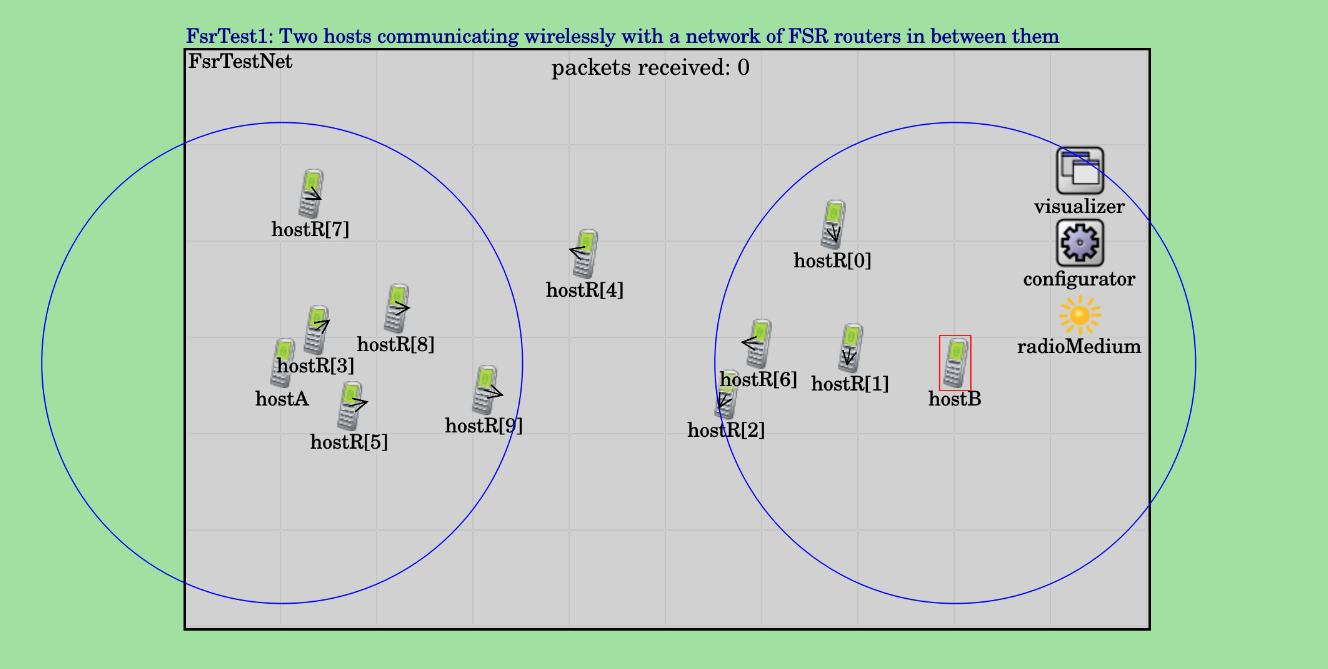
\includegraphics[width=\textwidth]{../figures/simulation_example.png}
    \caption{Simulation environment in OMNeT++}
    \label{fig:sim_env}
\end{figure}

The simulation runs for 90 seconds, with the first 2 seconds used for warm-up to allow the routing protocol to stabilize. Each study is run with 30 replications to ensure statistical significance, and the mean is taken along with 95\% confidence intervals.

The parameters varied in the simulation are link capacity, message length, message send interval, relay nodes count, and mobility speed. Studies vary a single variable while keeping the others constant. In each study, the non-varied parameters use these default values:
\begin{itemize}
    \item Link capacity: 8 Mbps
    \item Message length: 1000 bytes
    \item Message send interval: 150 milliseconds (mean of exponential distribution)
    \item Relay nodes count: 10
    \item Mobility speed: 10 to 20 m/s (uniformly distributed)
\end{itemize}

Each study also tests four different configurations of the FSR protocol, with different periods for the scope updates. All of them have three scopes except the last one, which has only one, to represent Global State Routing (GSR). The scope update periods are as follows:
\begin{itemize}
    \item 250, 500, 750ms
    \item 500, 750, 1000ms
    \item 750, 1500, 2250ms
    \item 500ms (GSR)
\end{itemize}

The performance metrics collected include end-to-end throughput, end-to-end delay, packet delivery ratio, data bits transmitted per data bit delivered (i.e. number of hops to reach destination), and control bits transmitted per data bit delivered. These metrics are taken from the simulation results generated by INET. For end-to-end throughput and delay, the values are taken directly from the UDP app module installed in the main hosts. The other metrics are calculated based on the packet sizes recorded in the \texttt{*.wlan[0].mac} module in all nodes, which records the packets transmitted to the radio medium.

\subsection{Results}

\subsubsection{Link capacity}
Figure \ref{fig:bitrate} shows the effects of link capacity on various metrics.

Higher link capacities lead to higher throughput, although the effect is not that significant for values higher than 2 Mbps, as seen in Figure \ref{fig:tput_bitrate}. The insignificant but still increasing effect past that point might be related to efficiency in the transmission of control packets.

Link capacity has a direct effect on lowering delay. The effect is diminished as the capacity increases past 4 Mbps however.

As with throughput, the packet delivery ratio increases with higher link capacity up to a certain optimal point, then it levels off.

The ratio of data bits transmitted per bit delivered is higher for lower link capacities, as shown in Figure \ref{fig:data_bits_bitrate}. This is expected, as higher link capacities allow for more efficient transmission of data packets, leading to fewer retransmissions before routes change.

For control bits transmitted per data bit delivered, the effect is similar to that of data bits, as shown in Figure \ref{fig:control_bits_bitrate}. What is interesting is the differences between the FSR configurations, where those with higher refresh rates resulted in a higher control-to-data ratio. As for the GSR configuration, it did not show much of a difference compared to the corresponding FSR configuration with the same update interval for the first scope (500ms). This might indicate that this simulation scenario relied greatly on first scopes, and that the second and third scopes did not affect the routing performance much.

\begin{figure}
    \centering
    \begin{subfigure}[b]{0.45\textwidth}
        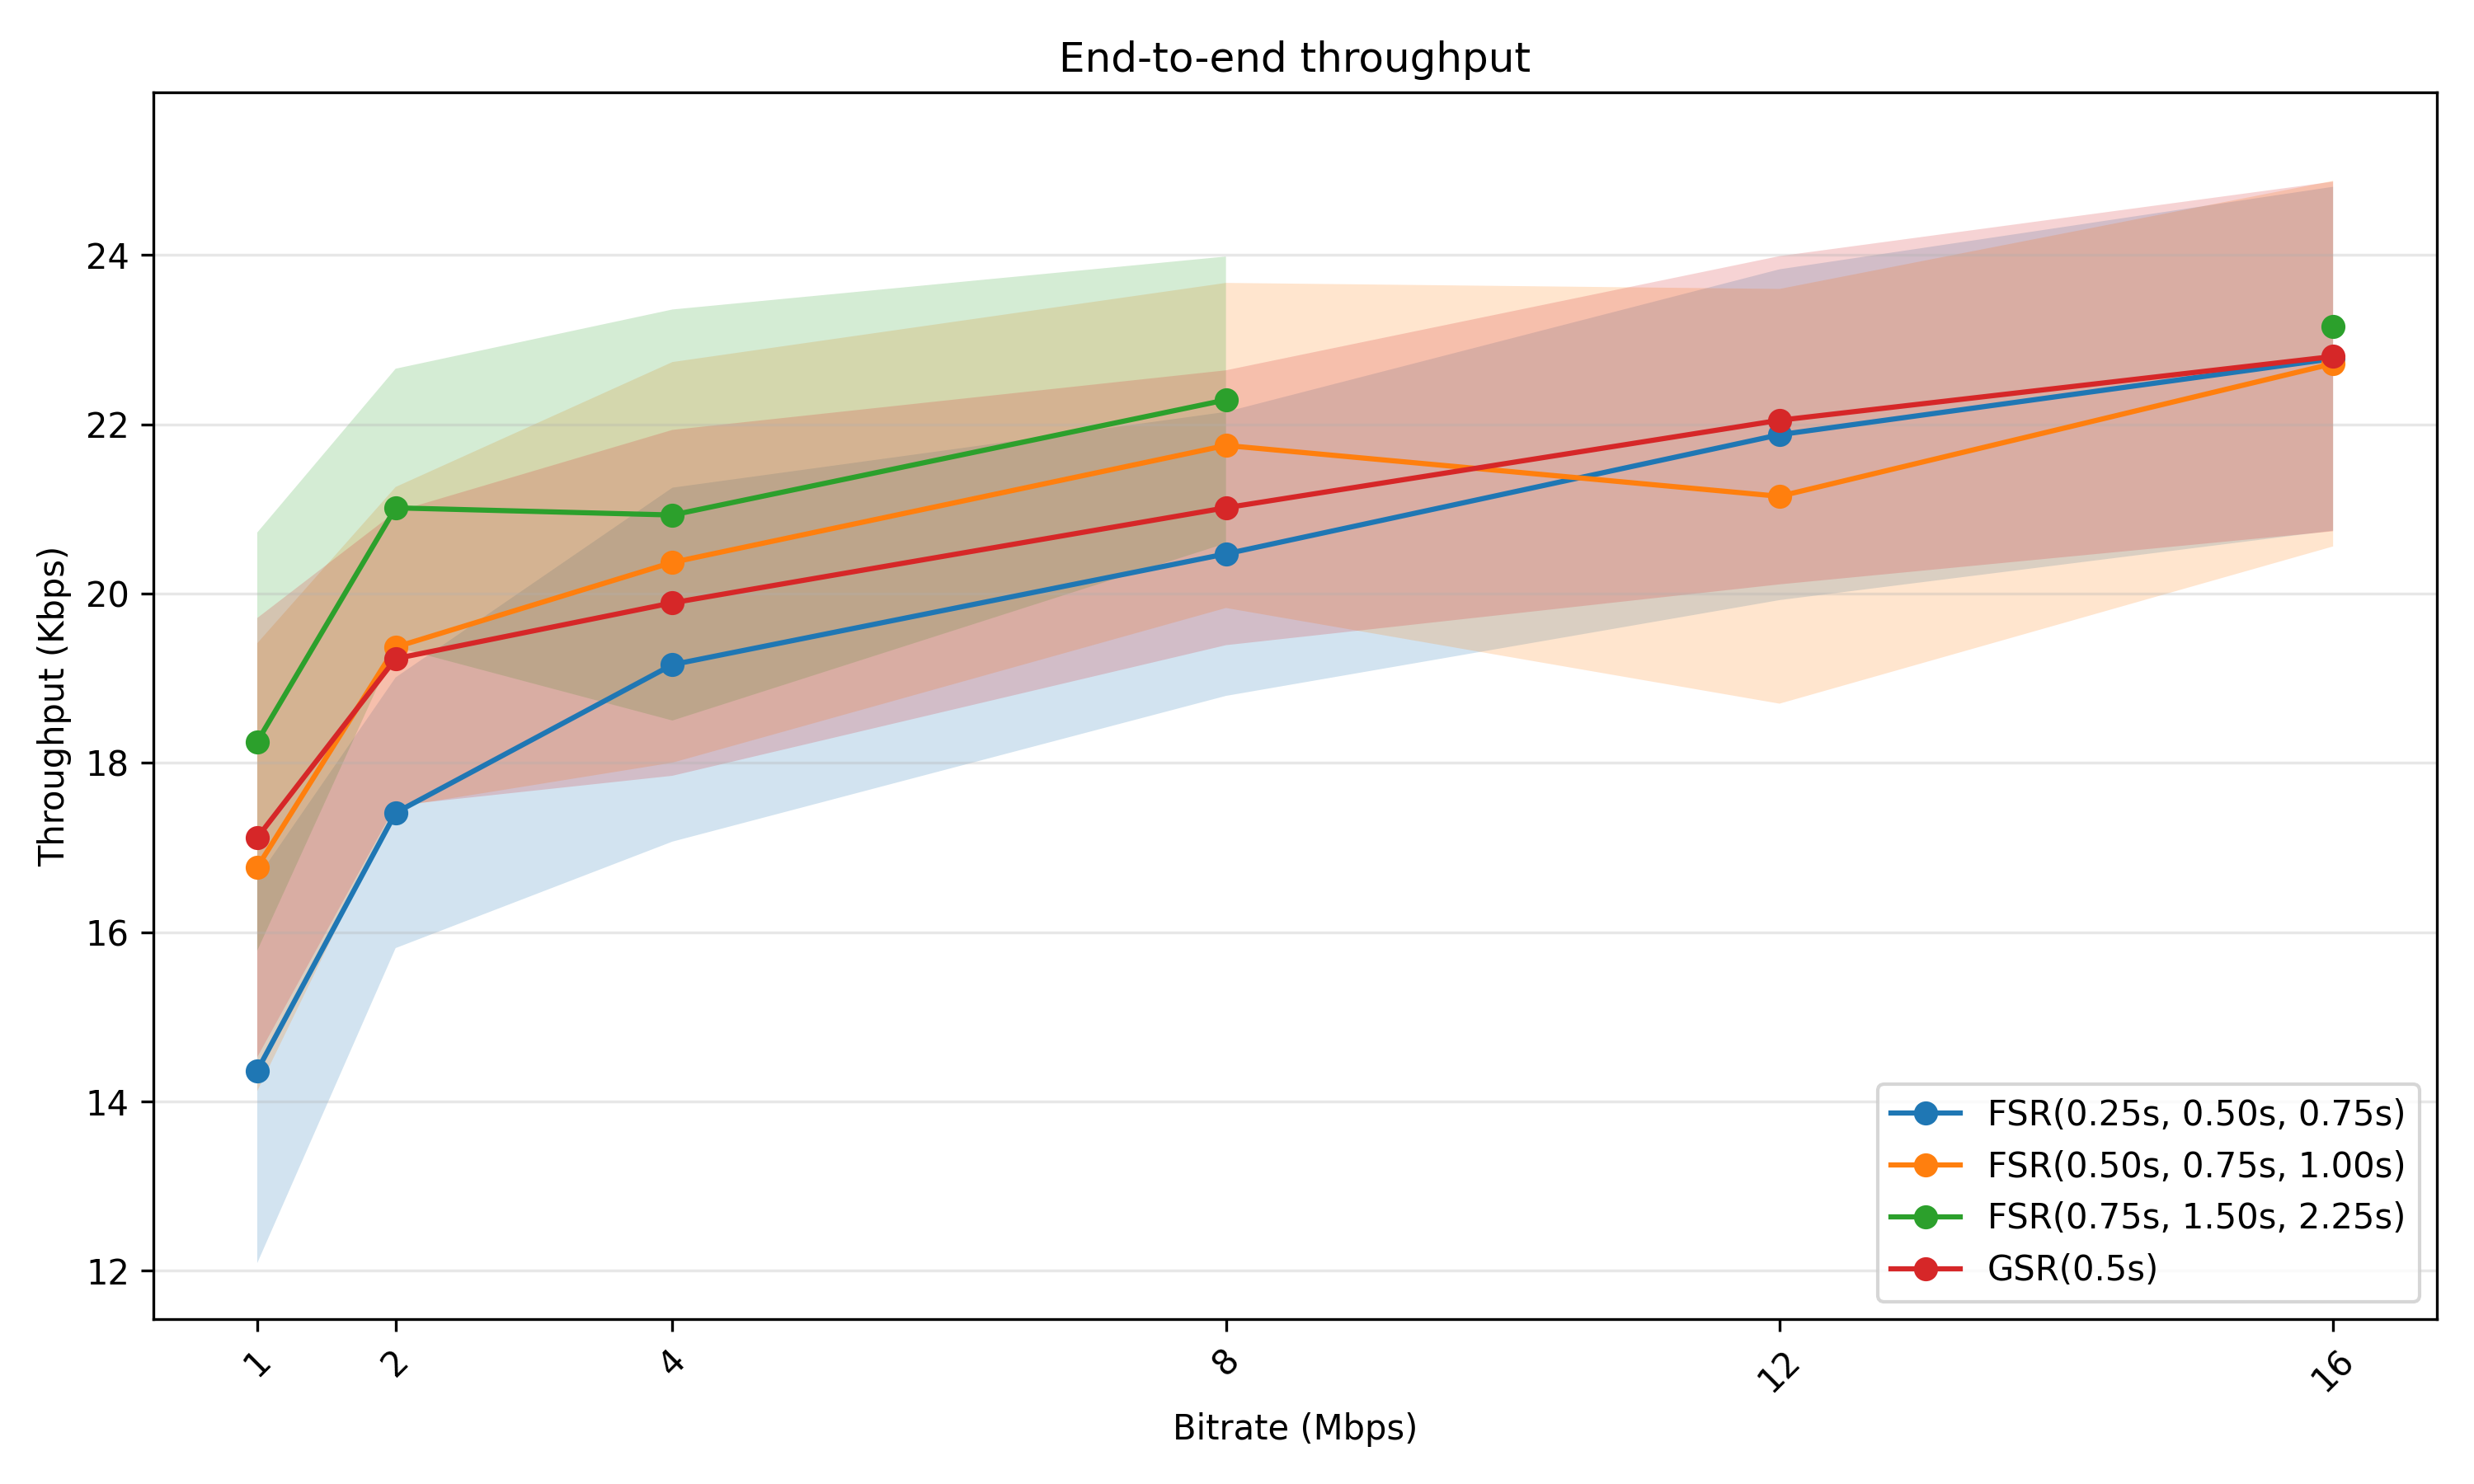
\includegraphics[width=\textwidth]{../figures/bitrate/end-to-end_throughput.png}
        \caption{End-to-end throughput}
        \label{fig:tput_bitrate}
    \end{subfigure}
    \hfill
    \begin{subfigure}[b]{0.45\textwidth}
        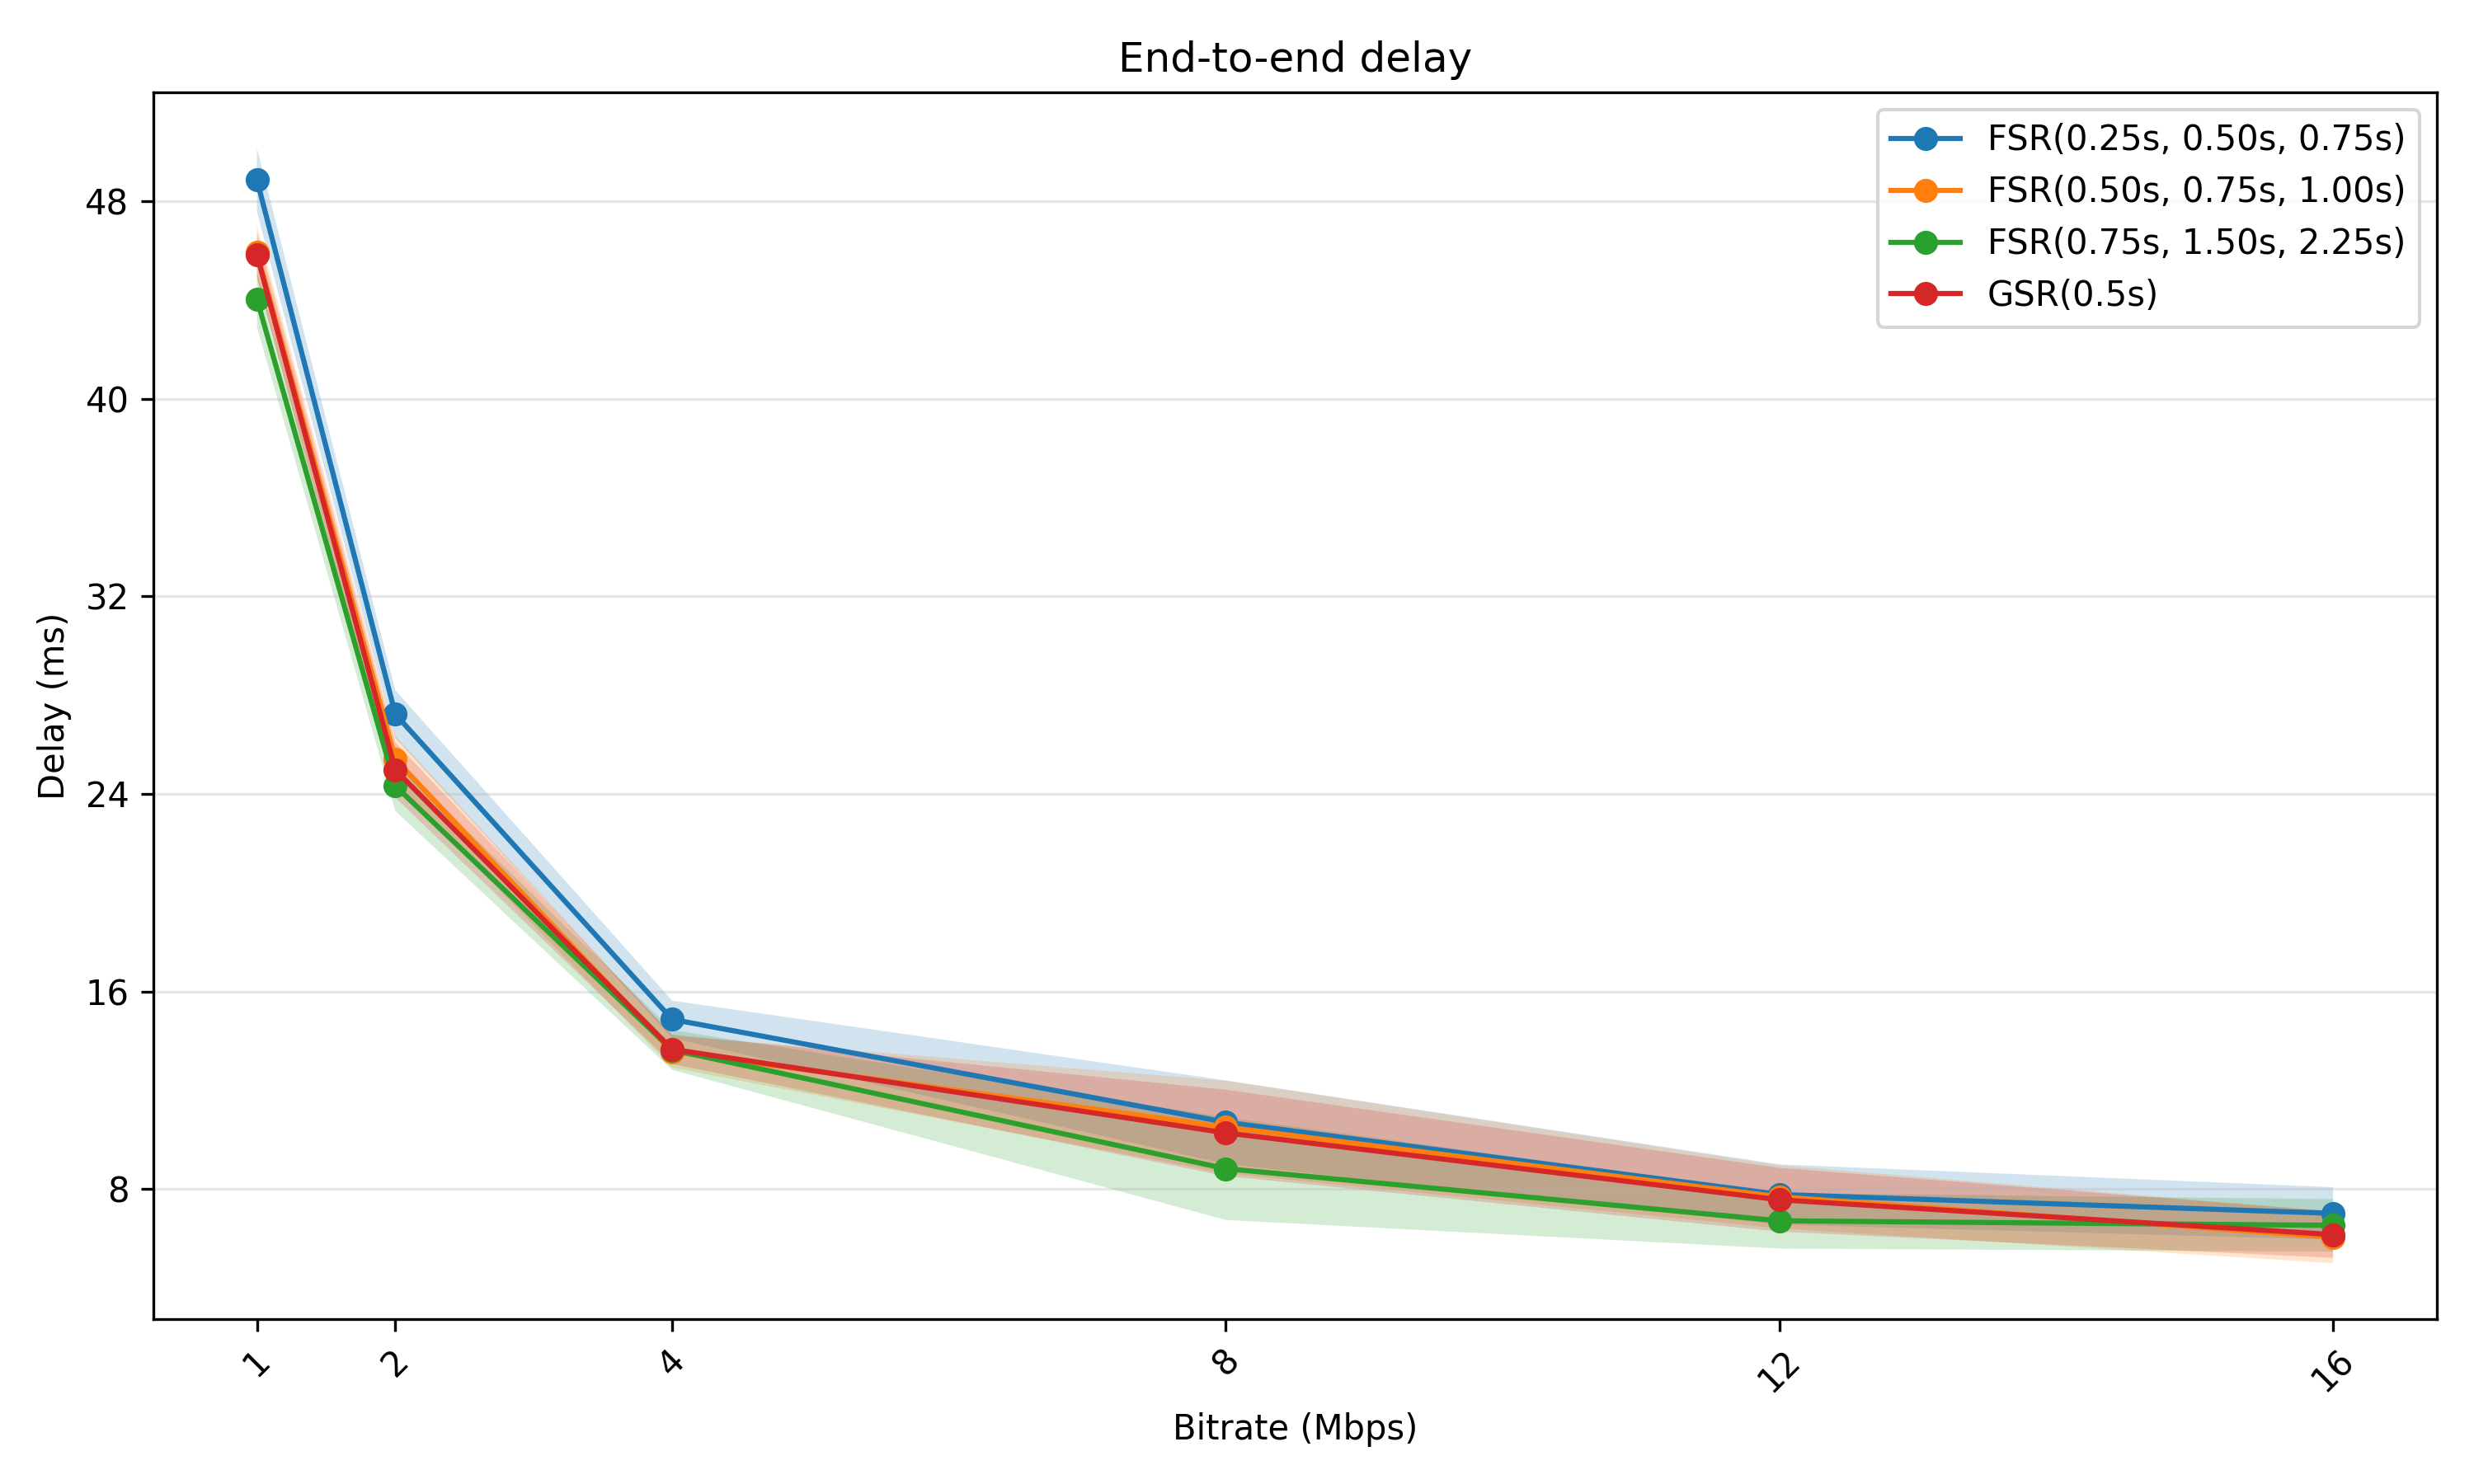
\includegraphics[width=\textwidth]{../figures/bitrate/end-to-end_delay.png}
        \caption{End-to-end delay}
        \label{fig:delay_bitrate}
    \end{subfigure}
    \begin{subfigure}[b]{0.45\textwidth}
        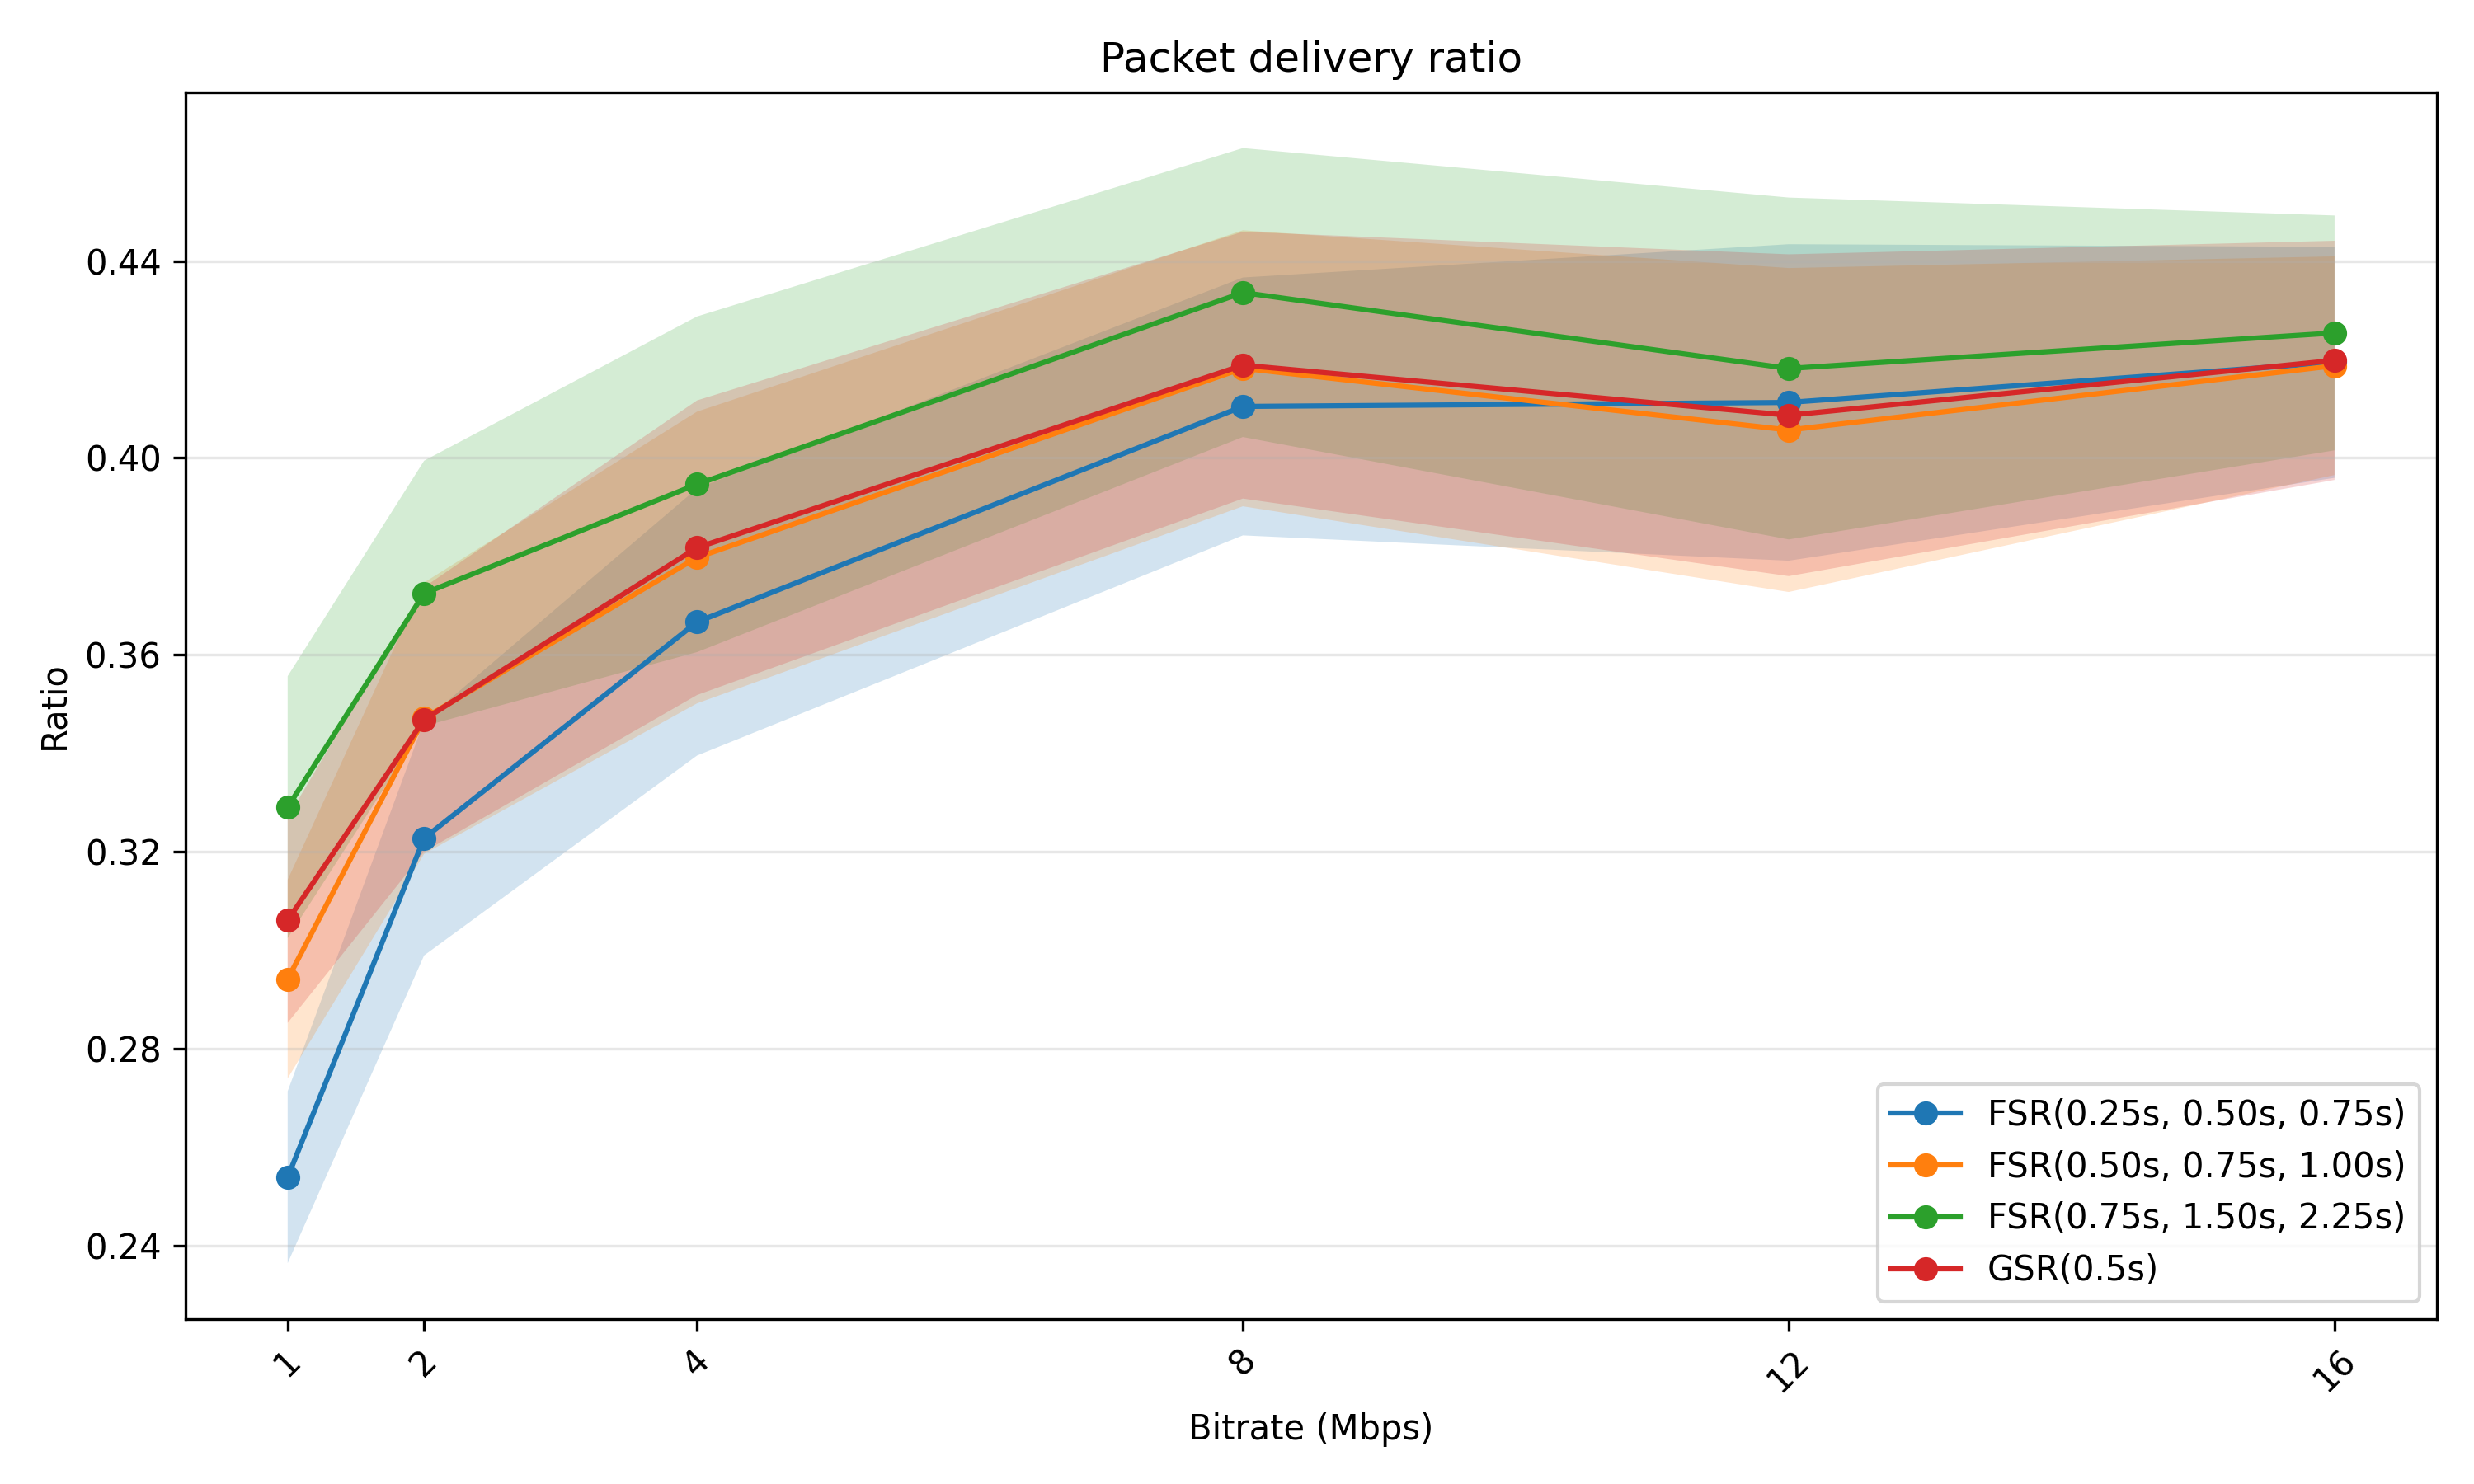
\includegraphics[width=\textwidth]{../figures/bitrate/packet_delivery_ratio.png}
        \caption{Packet delivery ratio}
        \label{fig:delivery_bitrate}
    \end{subfigure}
    \begin{subfigure}[b]{0.45\textwidth}
        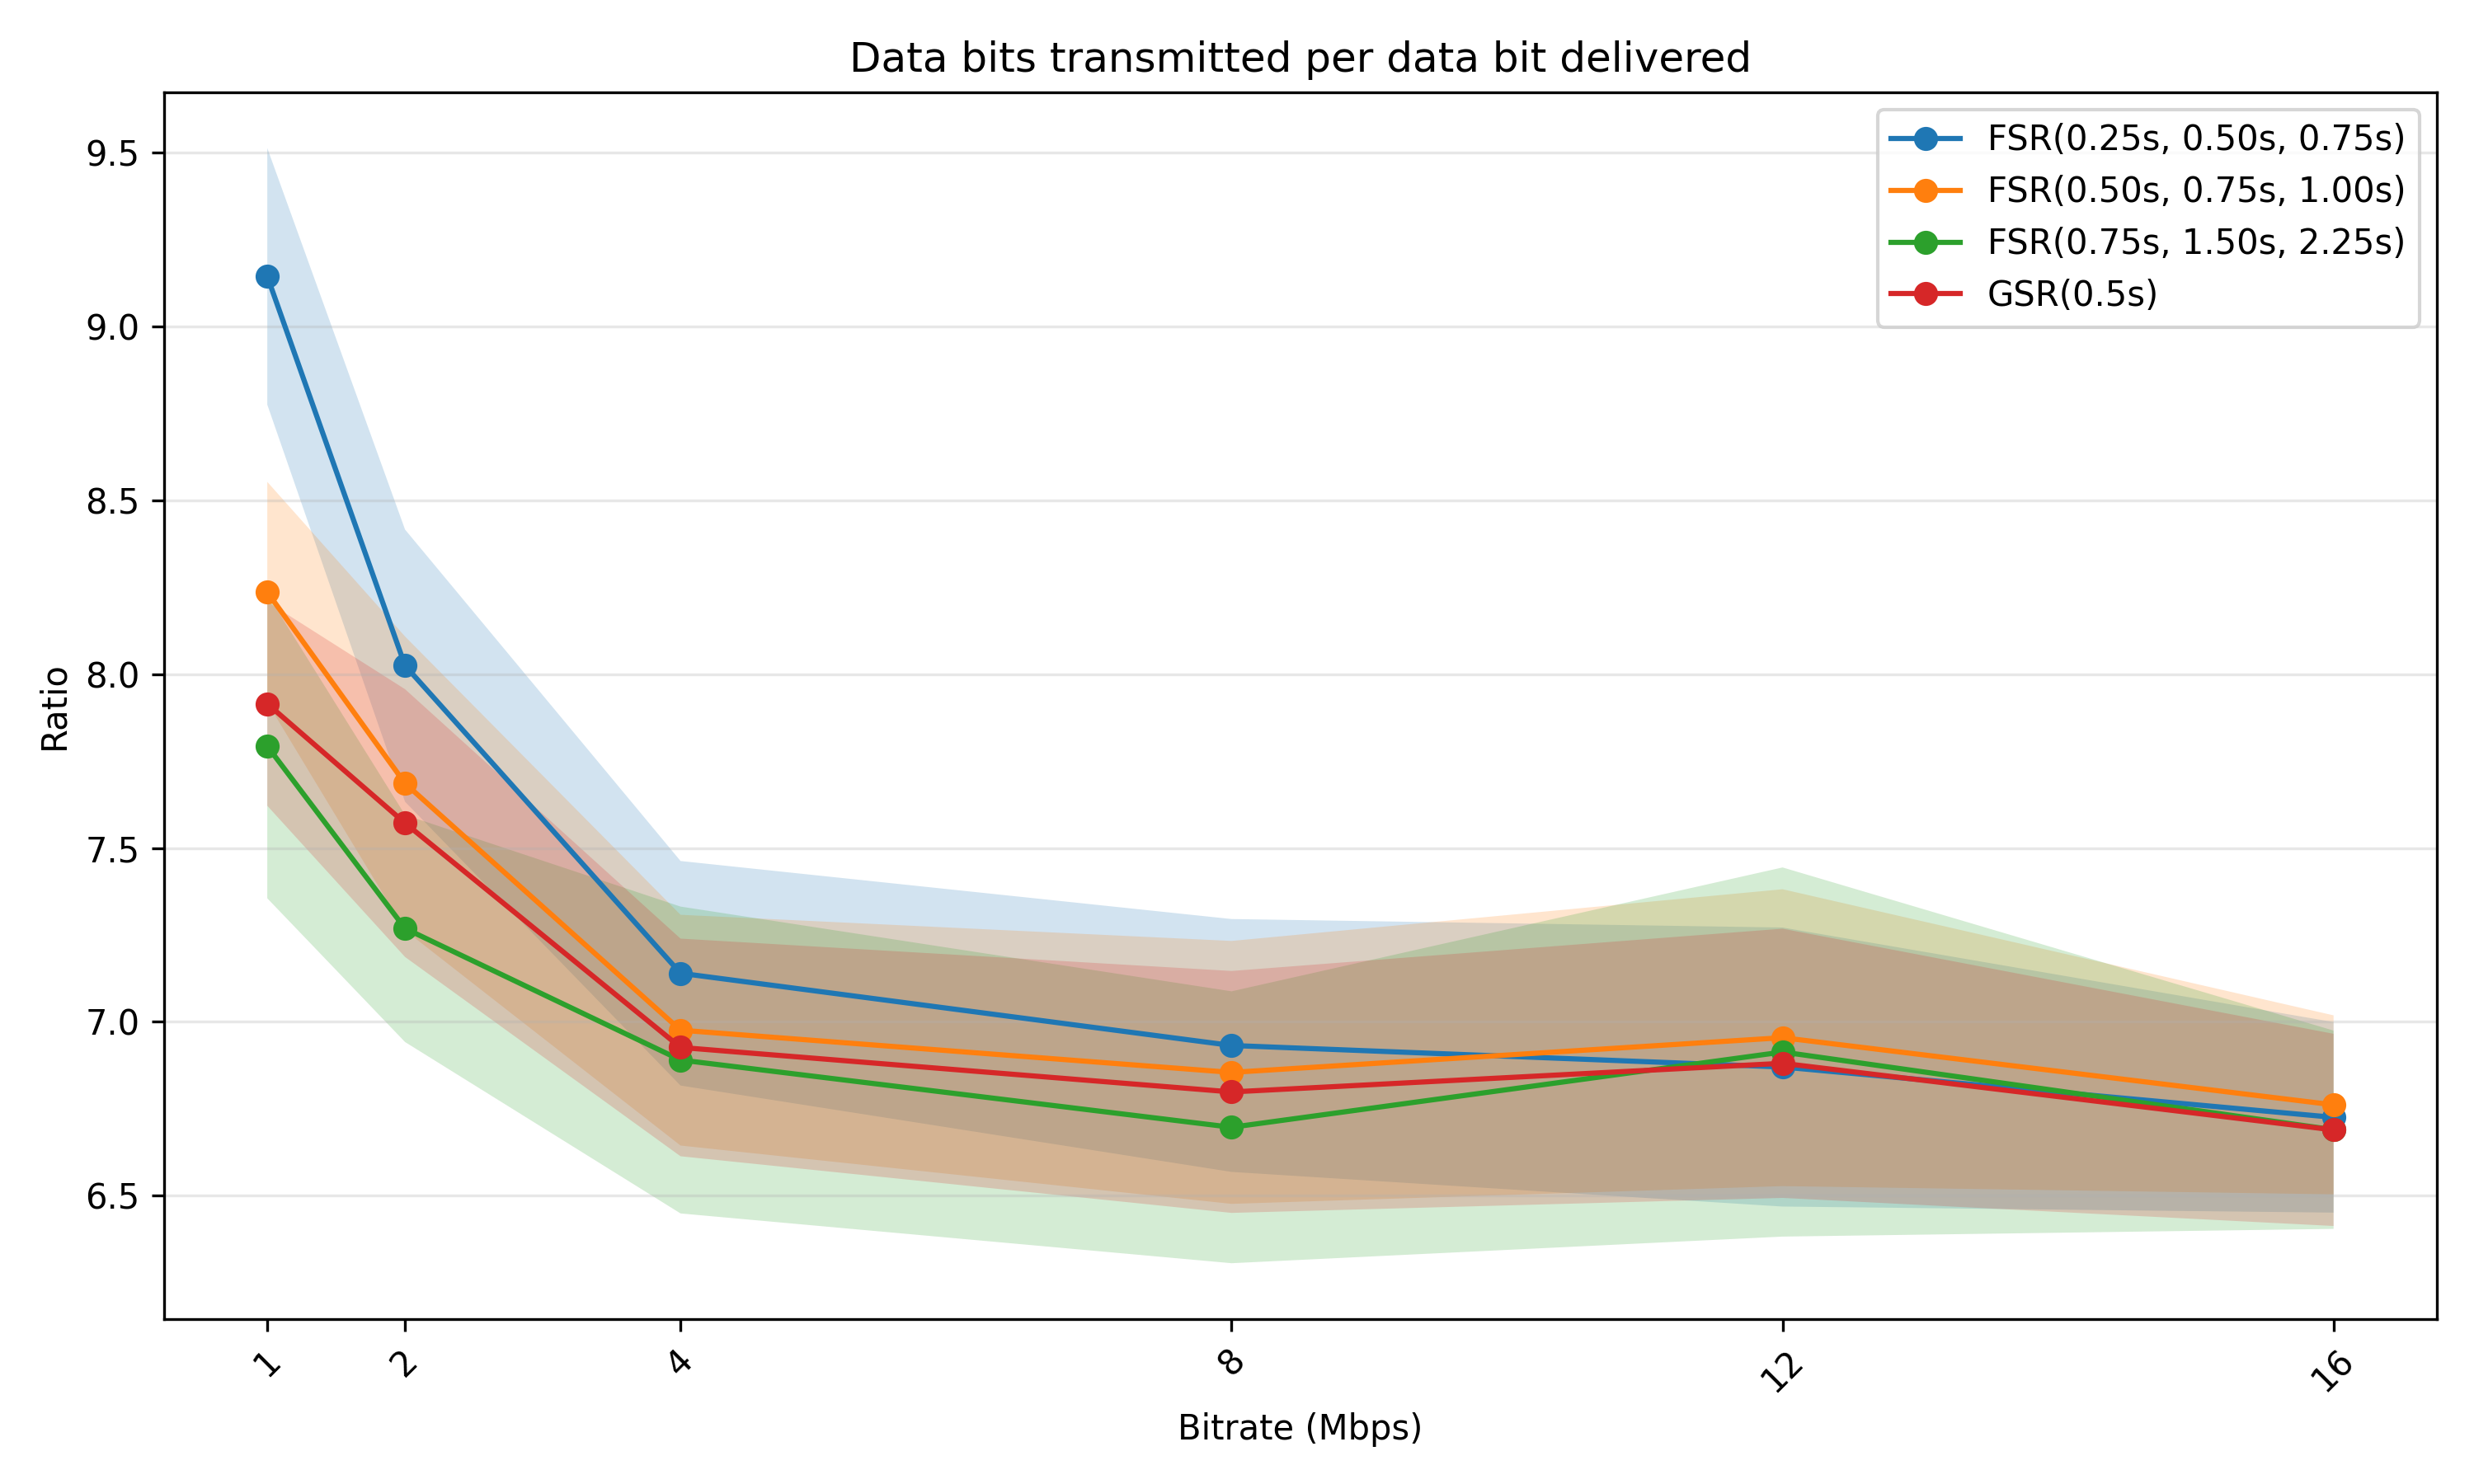
\includegraphics[width=\textwidth]{../figures/bitrate/data_bits_transmitted_per_data_bit_delivered.png}
        \caption{Data bits transmitted per data bit delivered}
        \label{fig:data_bits_bitrate}
    \end{subfigure}
    \begin{subfigure}[b]{0.45\textwidth}
        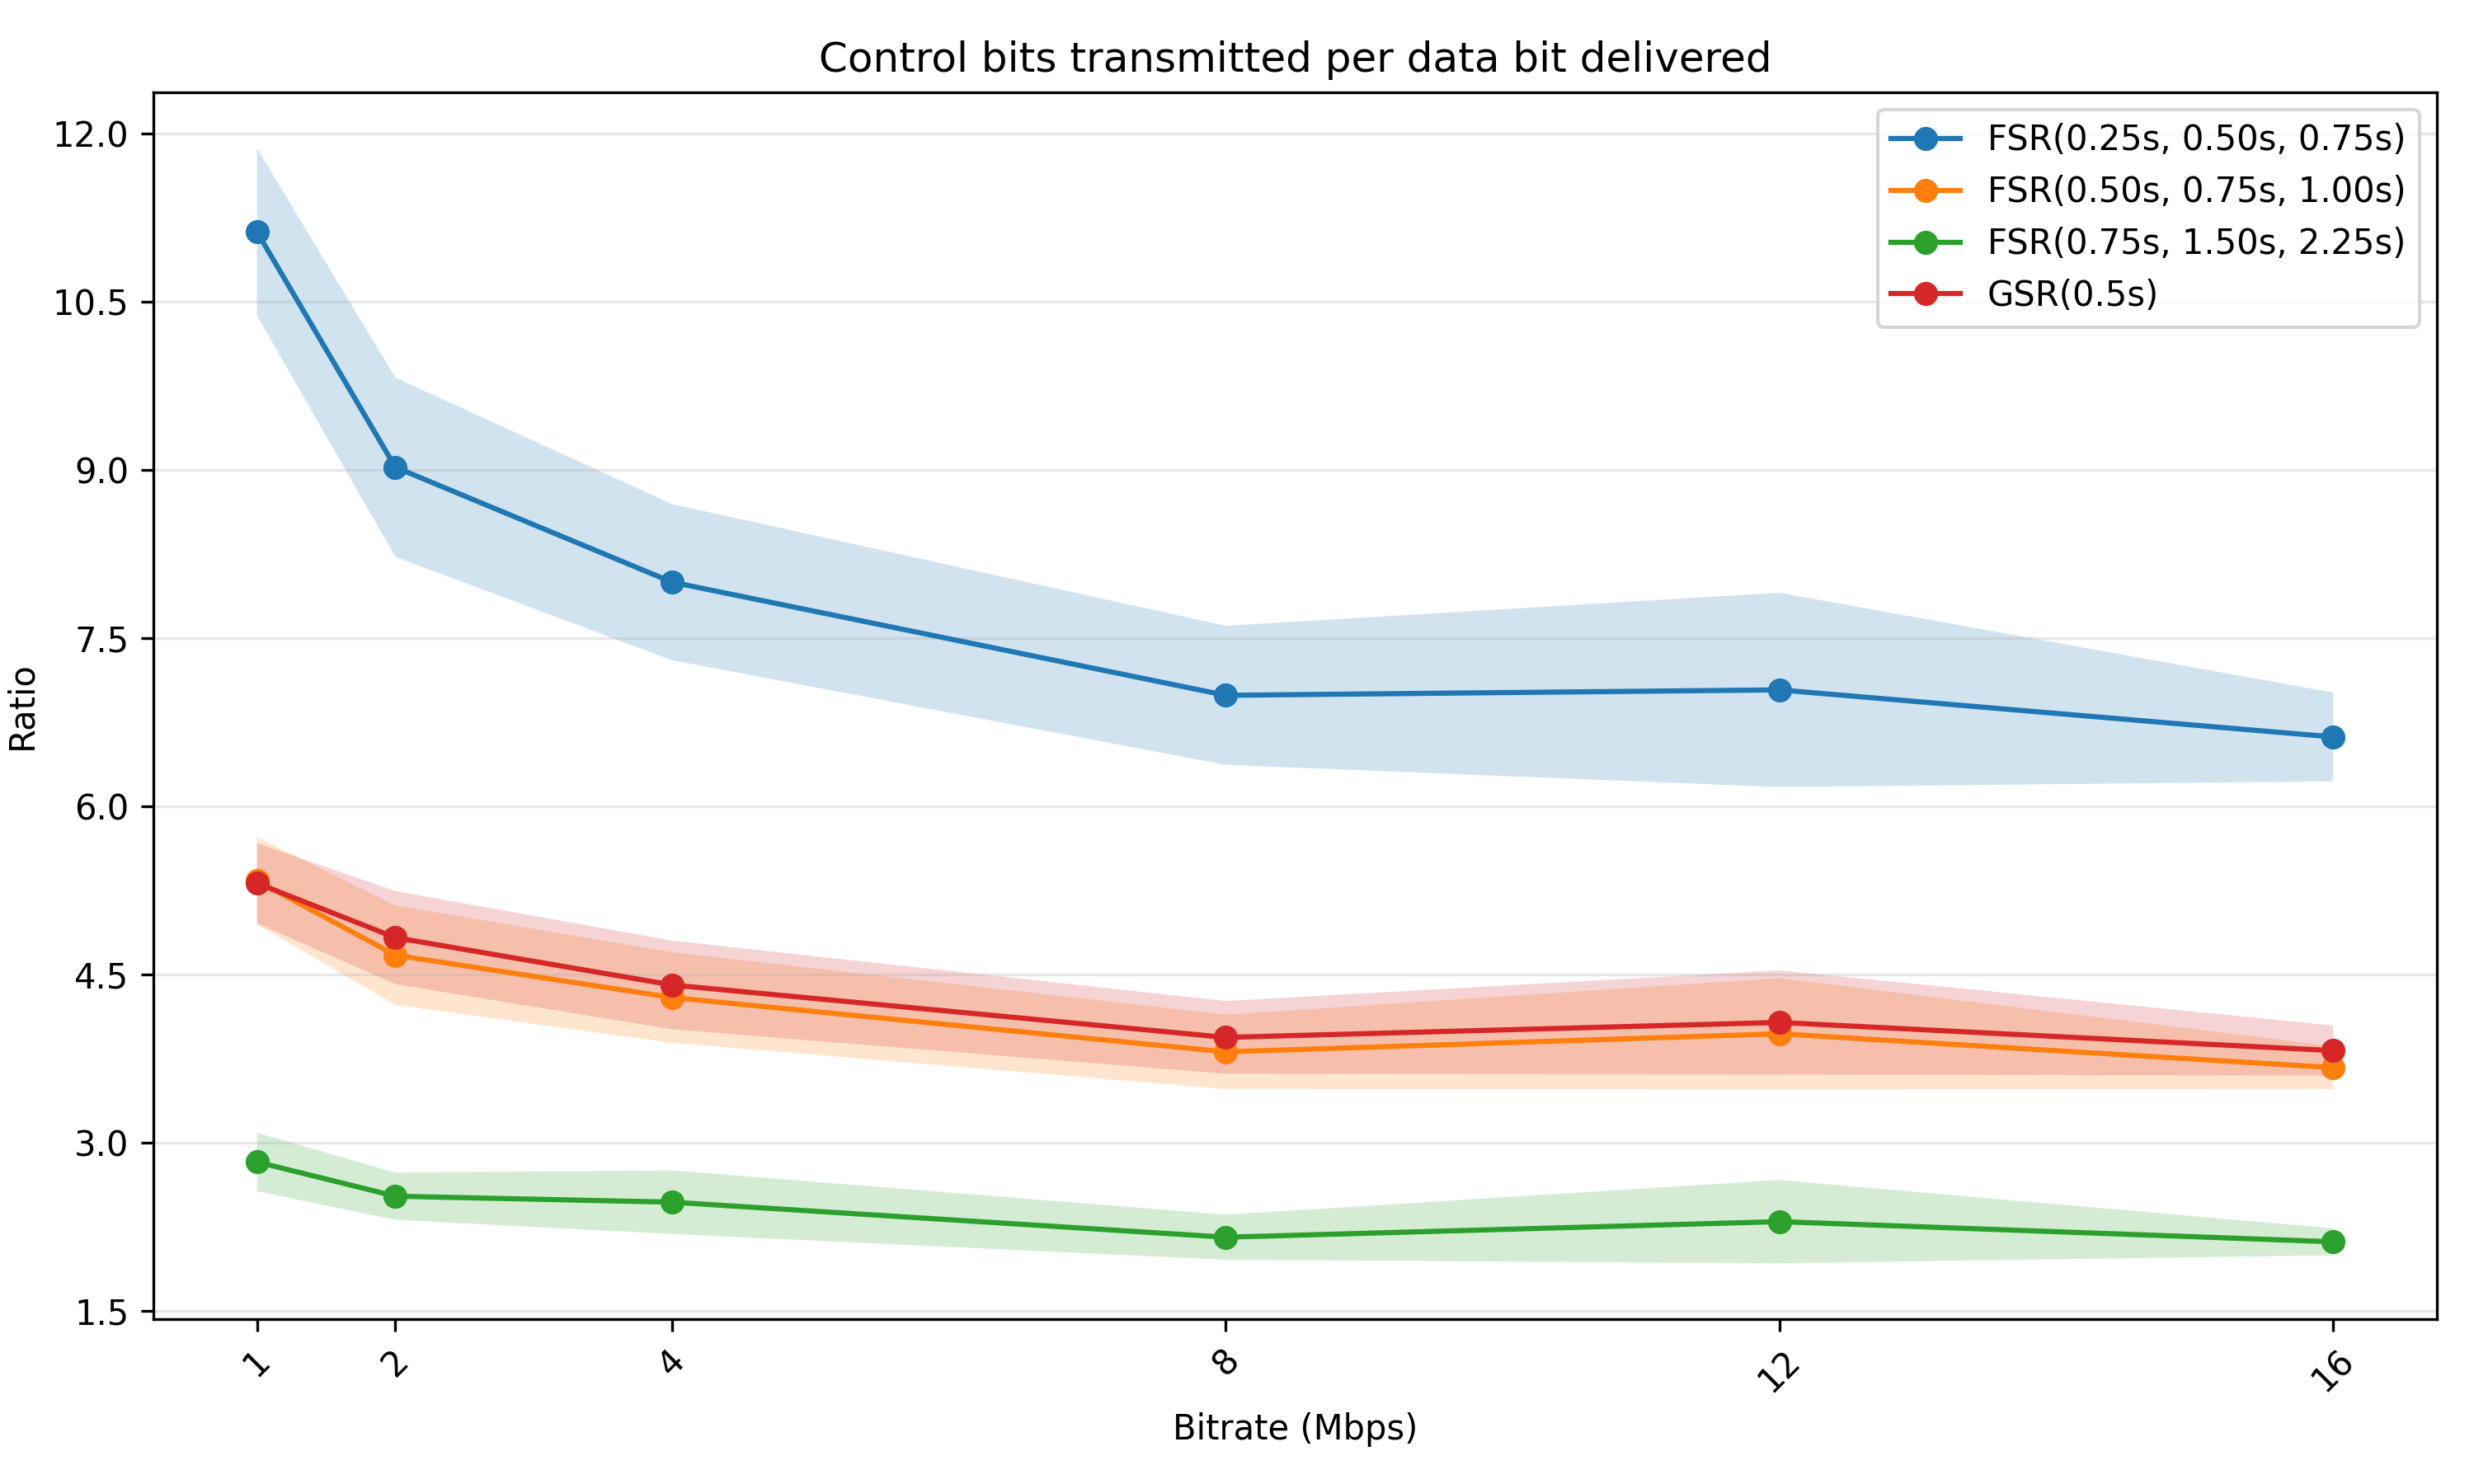
\includegraphics[width=\textwidth]{../figures/bitrate/control_bits_transmitted_per_data_bit_delivered.png}
        \caption{Control bits transmitted per data bit delivered}
        \label{fig:control_bits_bitrate}
    \end{subfigure}
    \caption{Link capacity (bitrate)}
    \label{fig:bitrate}
\end{figure}

\subsubsection{Node count}
Figure \ref{fig:node} shows the effects of node count on the tested metrics.

Throughput decreased with increasing node counts, as shown in Figure \ref{fig:tput_node}, possibly due to increased contention for the shared medium.

Node count has a negative effect on end-to-end delay. This is more noticeable in instances with more frequent FSR updates, as the least frequent FSR instance (750ms for the first scope) does not seem to suffer much from increased node counts. This seems to be a general trend with the other metrics too, where lower refresh rate results in better performance.

For the scenarios tested, it appears that a network size of 14 relay nodes is optimal, as higher node counts lead to lower packet delivery ratios, as shown in Figure \ref{fig:delivery_node}. This is likely due to increased contention for the shared medium, leading to more collisions and retransmissions. Lower node counts also result in worse performance as the number of relay nodes is not sufficient to maintain a stable route between the main hosts.

The data and control bit transmission ratios are larger for higher node counts, as shown in Figures \ref{fig:data_bits_node} and \ref{fig:control_bits_node}. This is expected, as more nodes lead to more hops in the route, resulting in more data and control bits transmitted. We can also see how much of a difference the scope update frequencies affect these results.


\begin{figure}
    \centering
    \begin{subfigure}[b]{0.45\textwidth}
        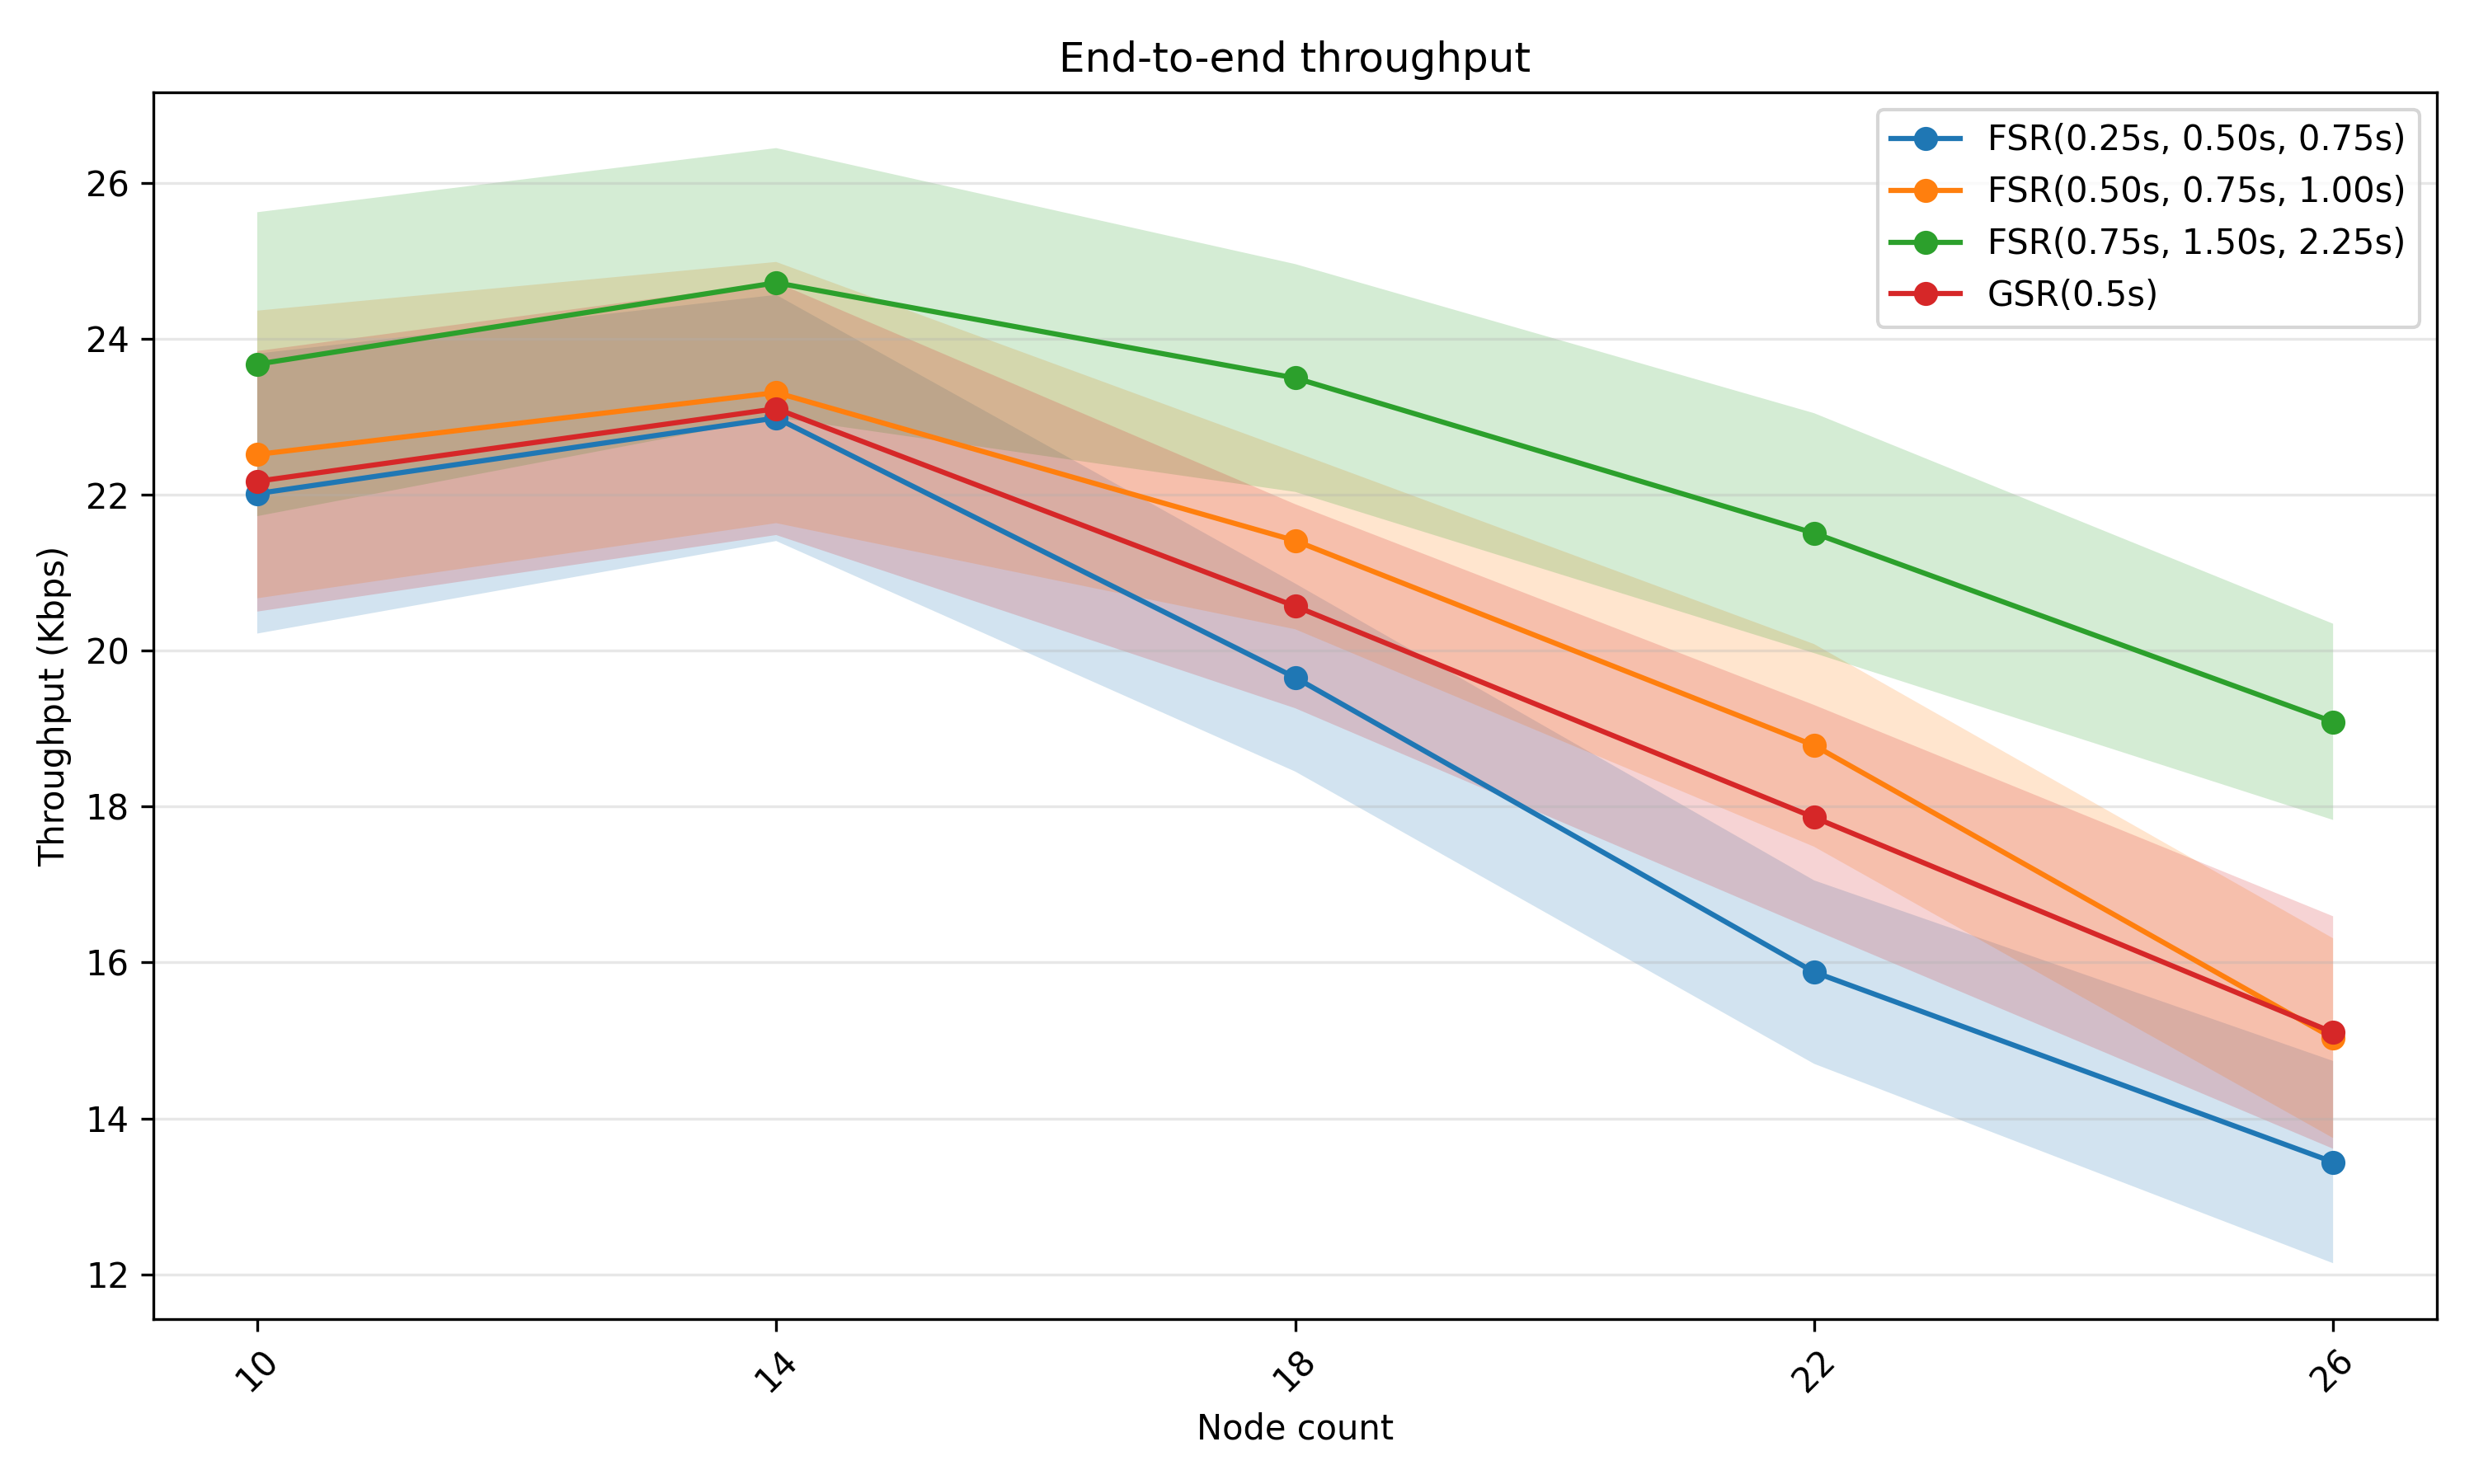
\includegraphics[width=\textwidth]{../figures/nodeCount/end-to-end_throughput.png}
        \caption{End-to-end throughput}
        \label{fig:tput_node}
    \end{subfigure}
    \hfill
    \begin{subfigure}[b]{0.45\textwidth}
        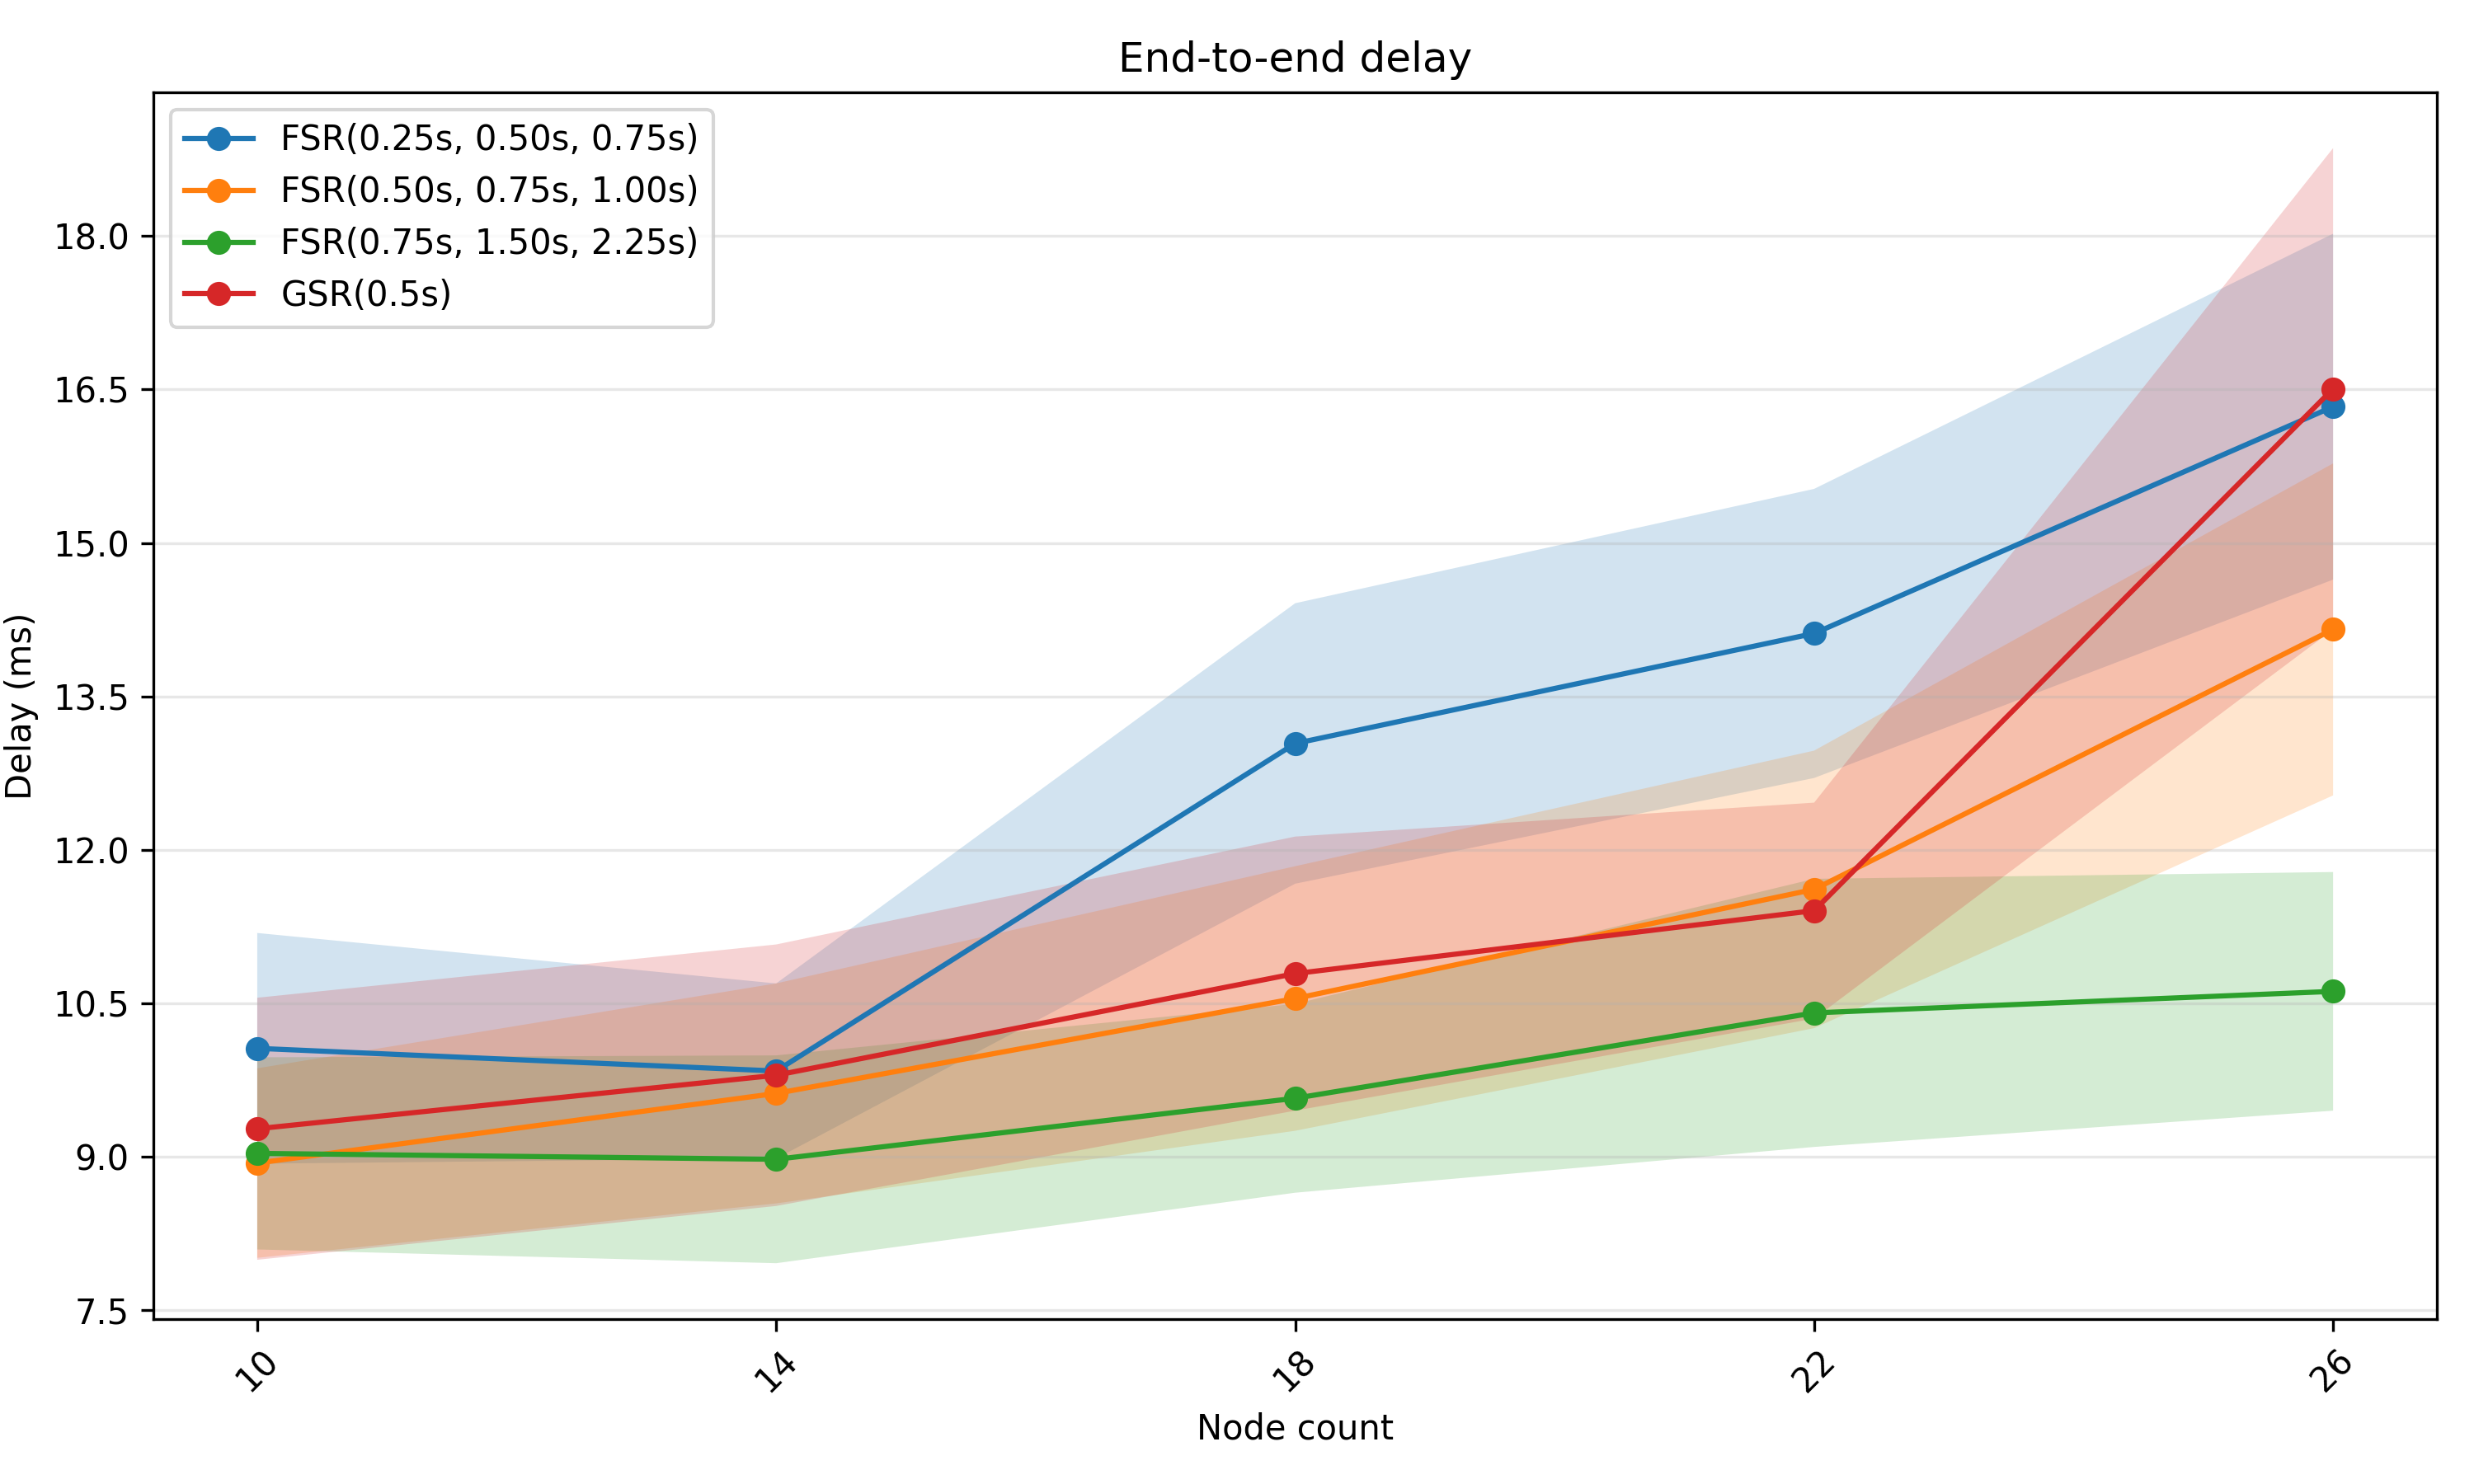
\includegraphics[width=\textwidth]{../figures/nodeCount/end-to-end_delay.png}
        \caption{End-to-end delay}
        \label{fig:delay_node}
    \end{subfigure}
    \begin{subfigure}[b]{0.45\textwidth}
        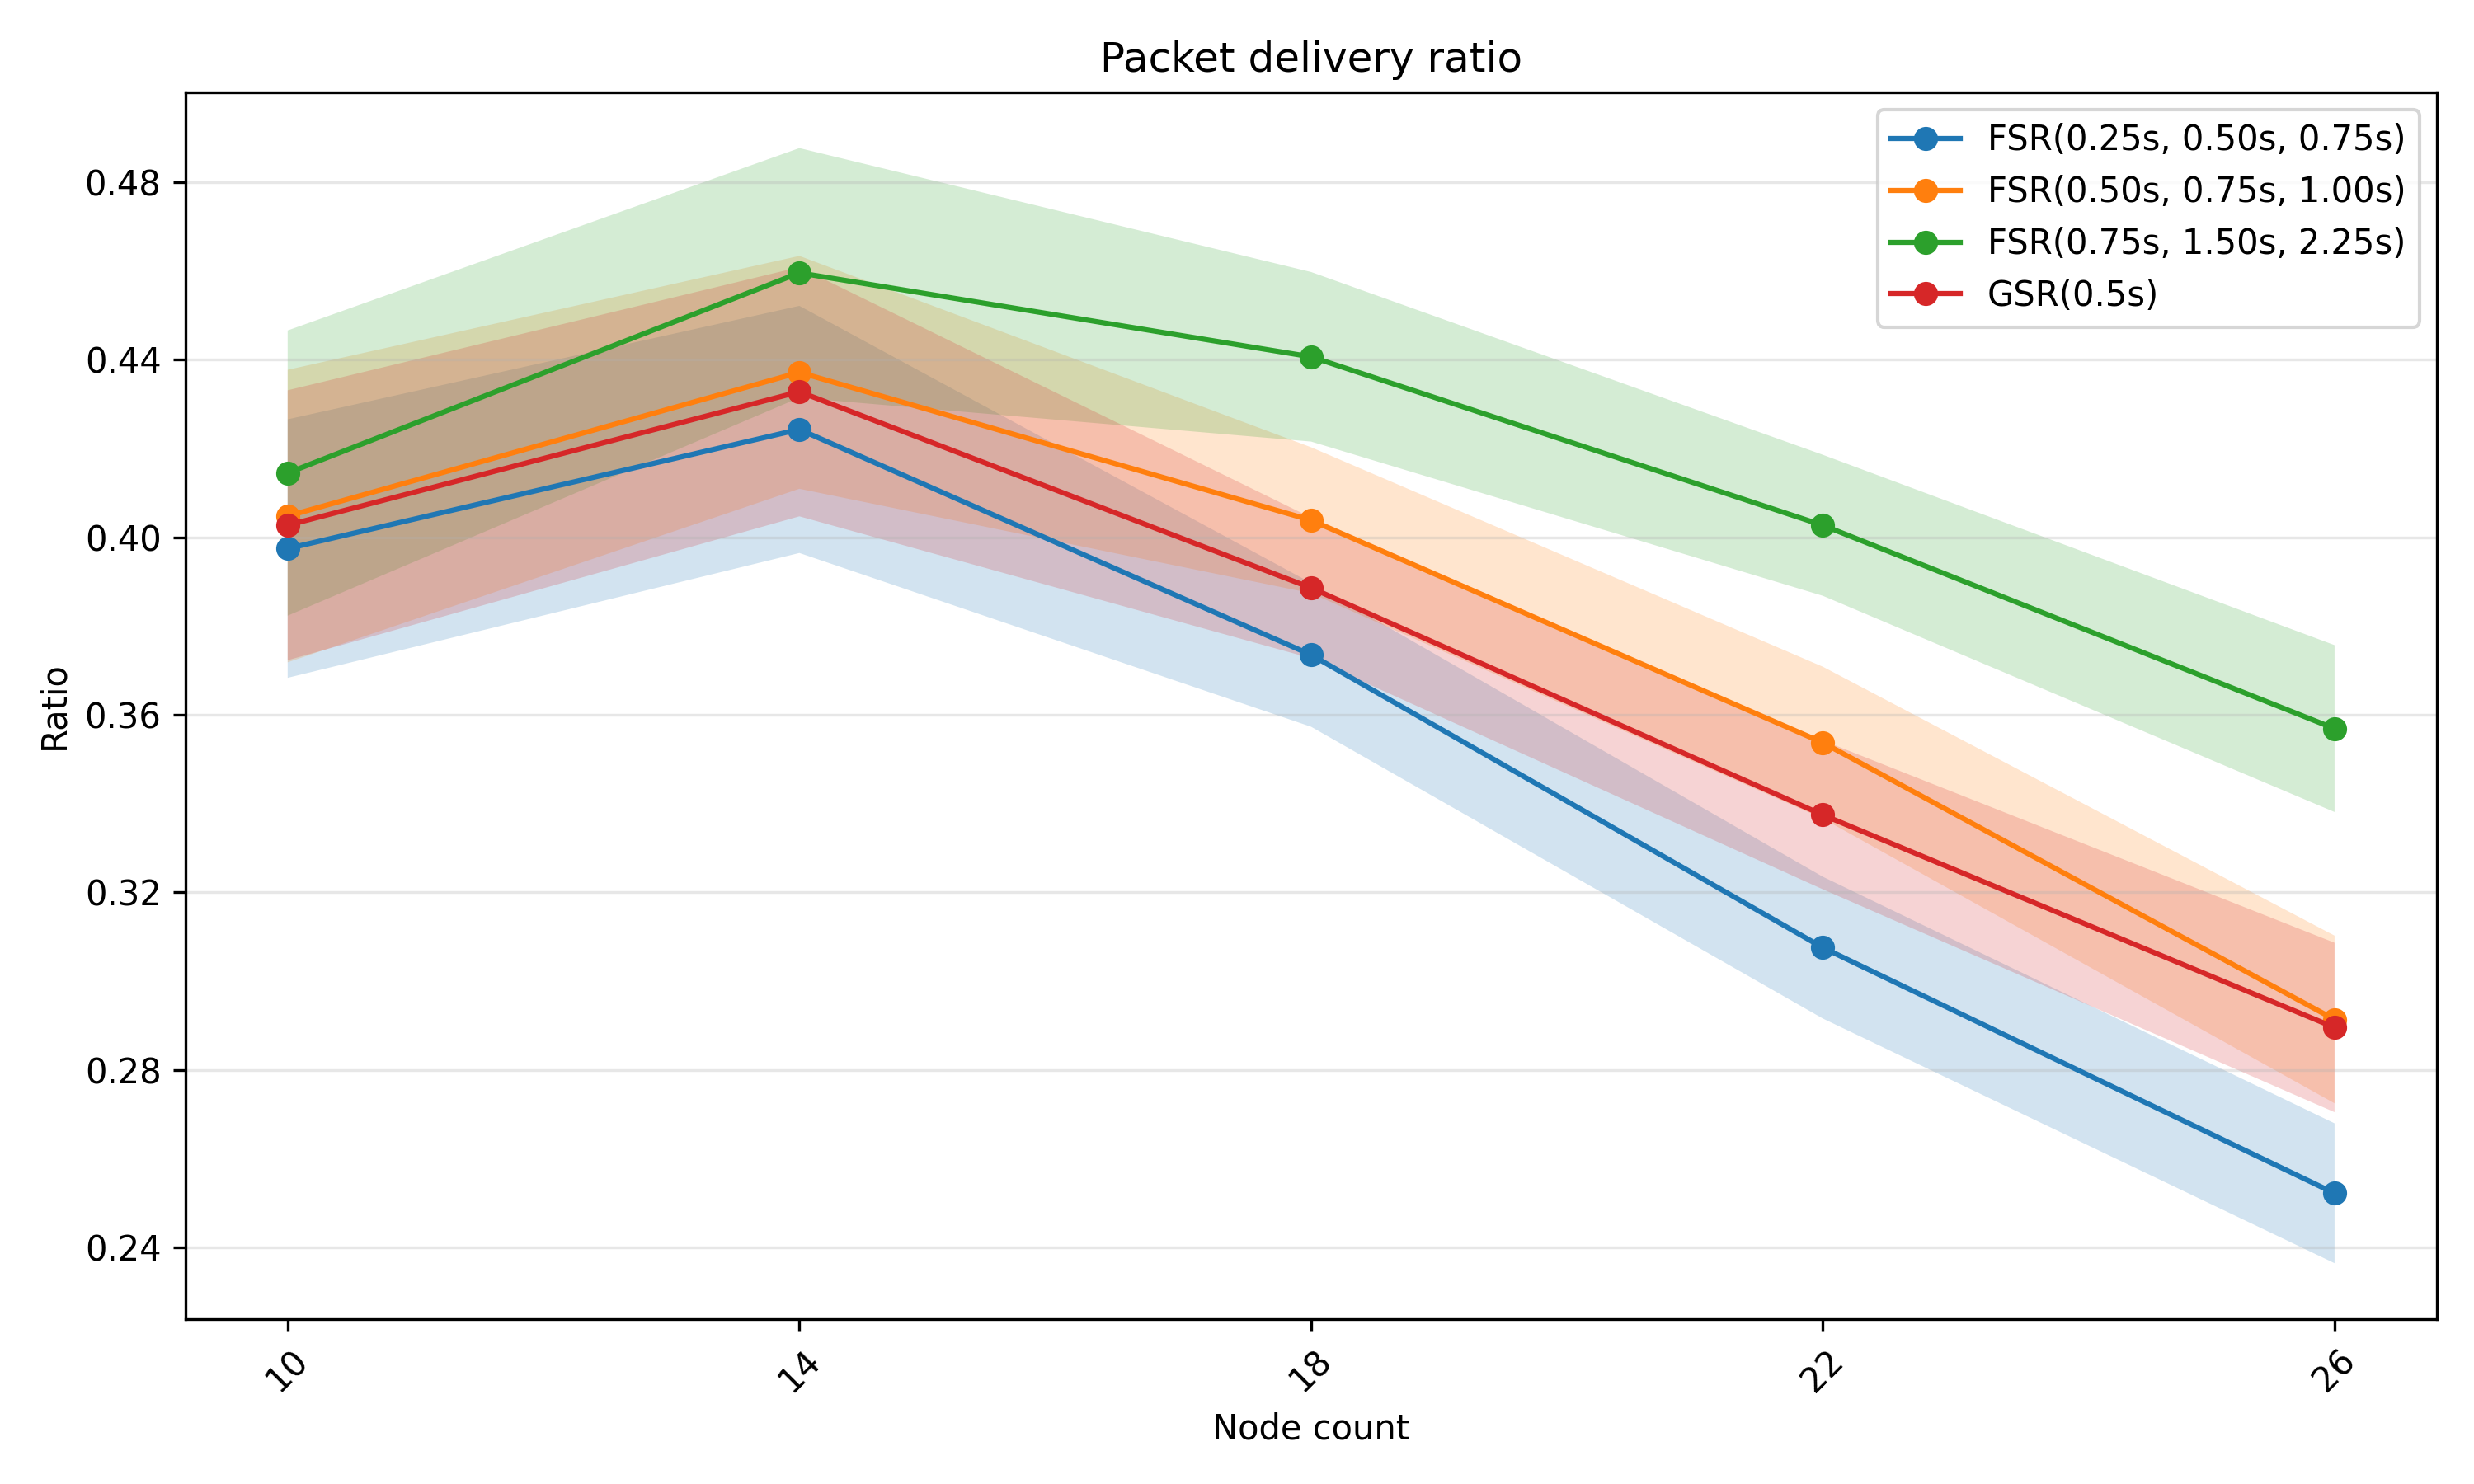
\includegraphics[width=\textwidth]{../figures/nodeCount/packet_delivery_ratio.png}
        \caption{Packet delivery ratio}
        \label{fig:delivery_node}
    \end{subfigure}
    \begin{subfigure}[b]{0.45\textwidth}
        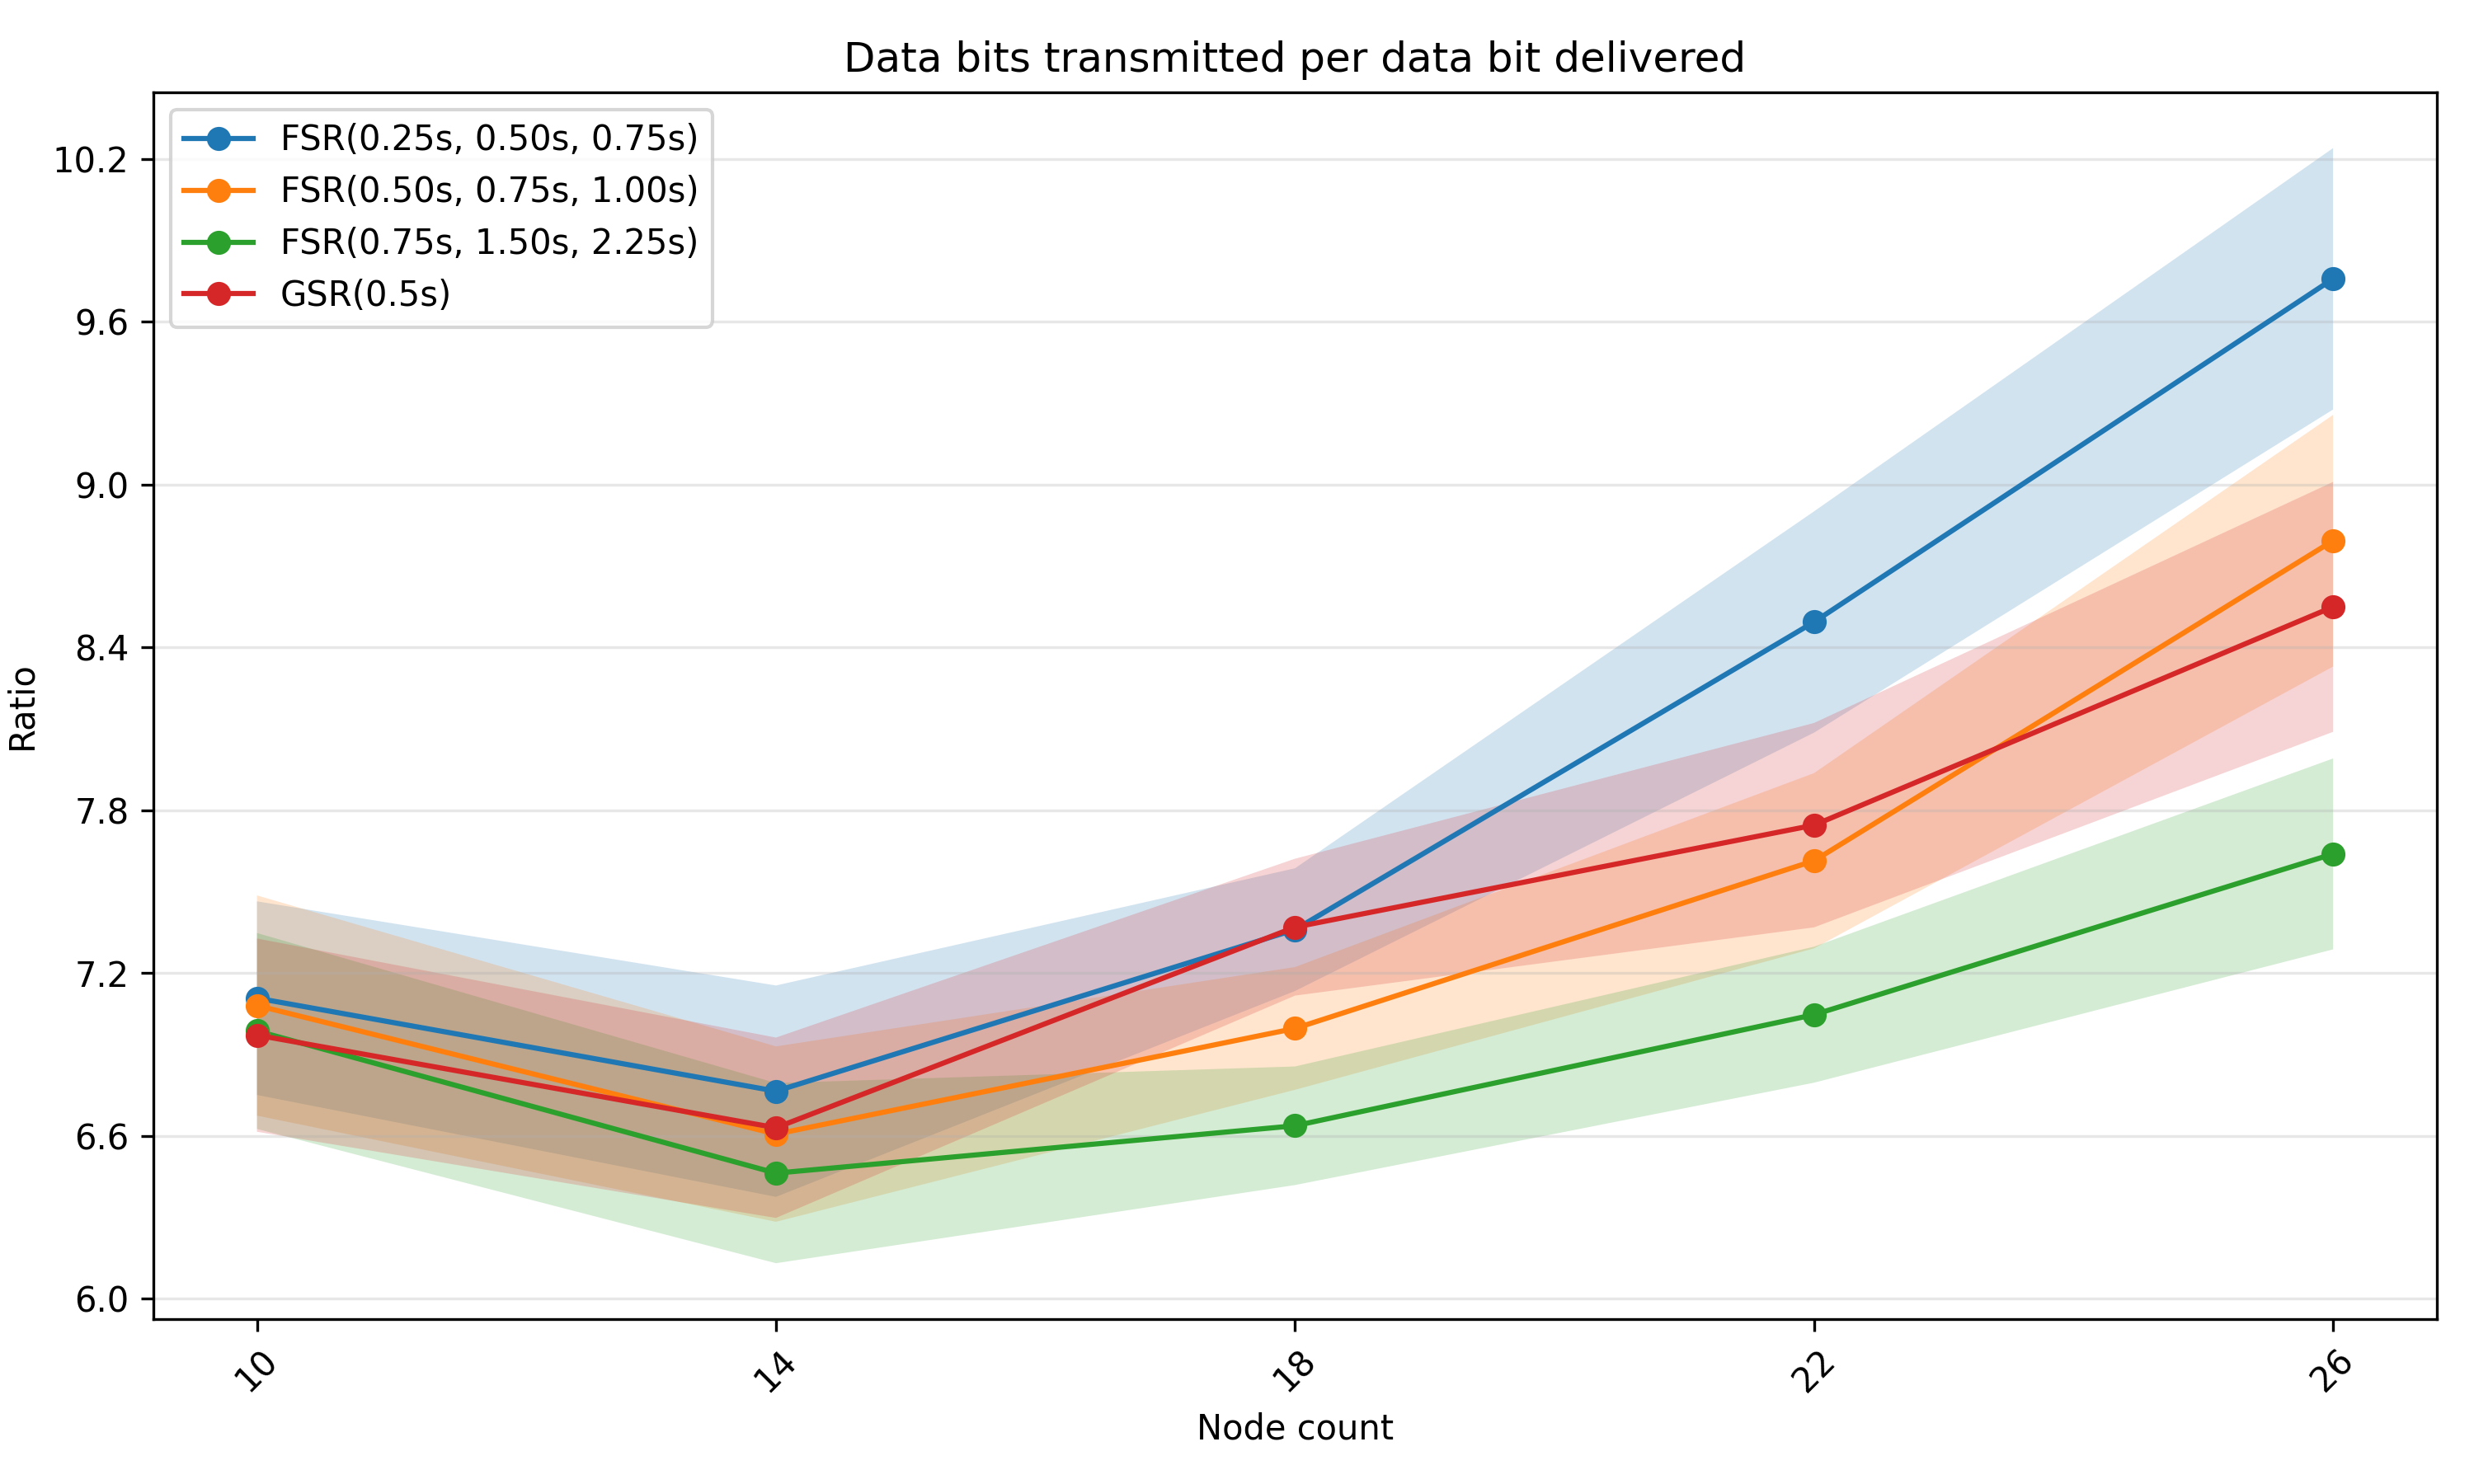
\includegraphics[width=\textwidth]{../figures/nodeCount/data_bits_transmitted_per_data_bit_delivered.png}
        \caption{Data bits transmitted per data bit delivered}
        \label{fig:data_bits_node}
    \end{subfigure}
    \begin{subfigure}[b]{0.45\textwidth}
        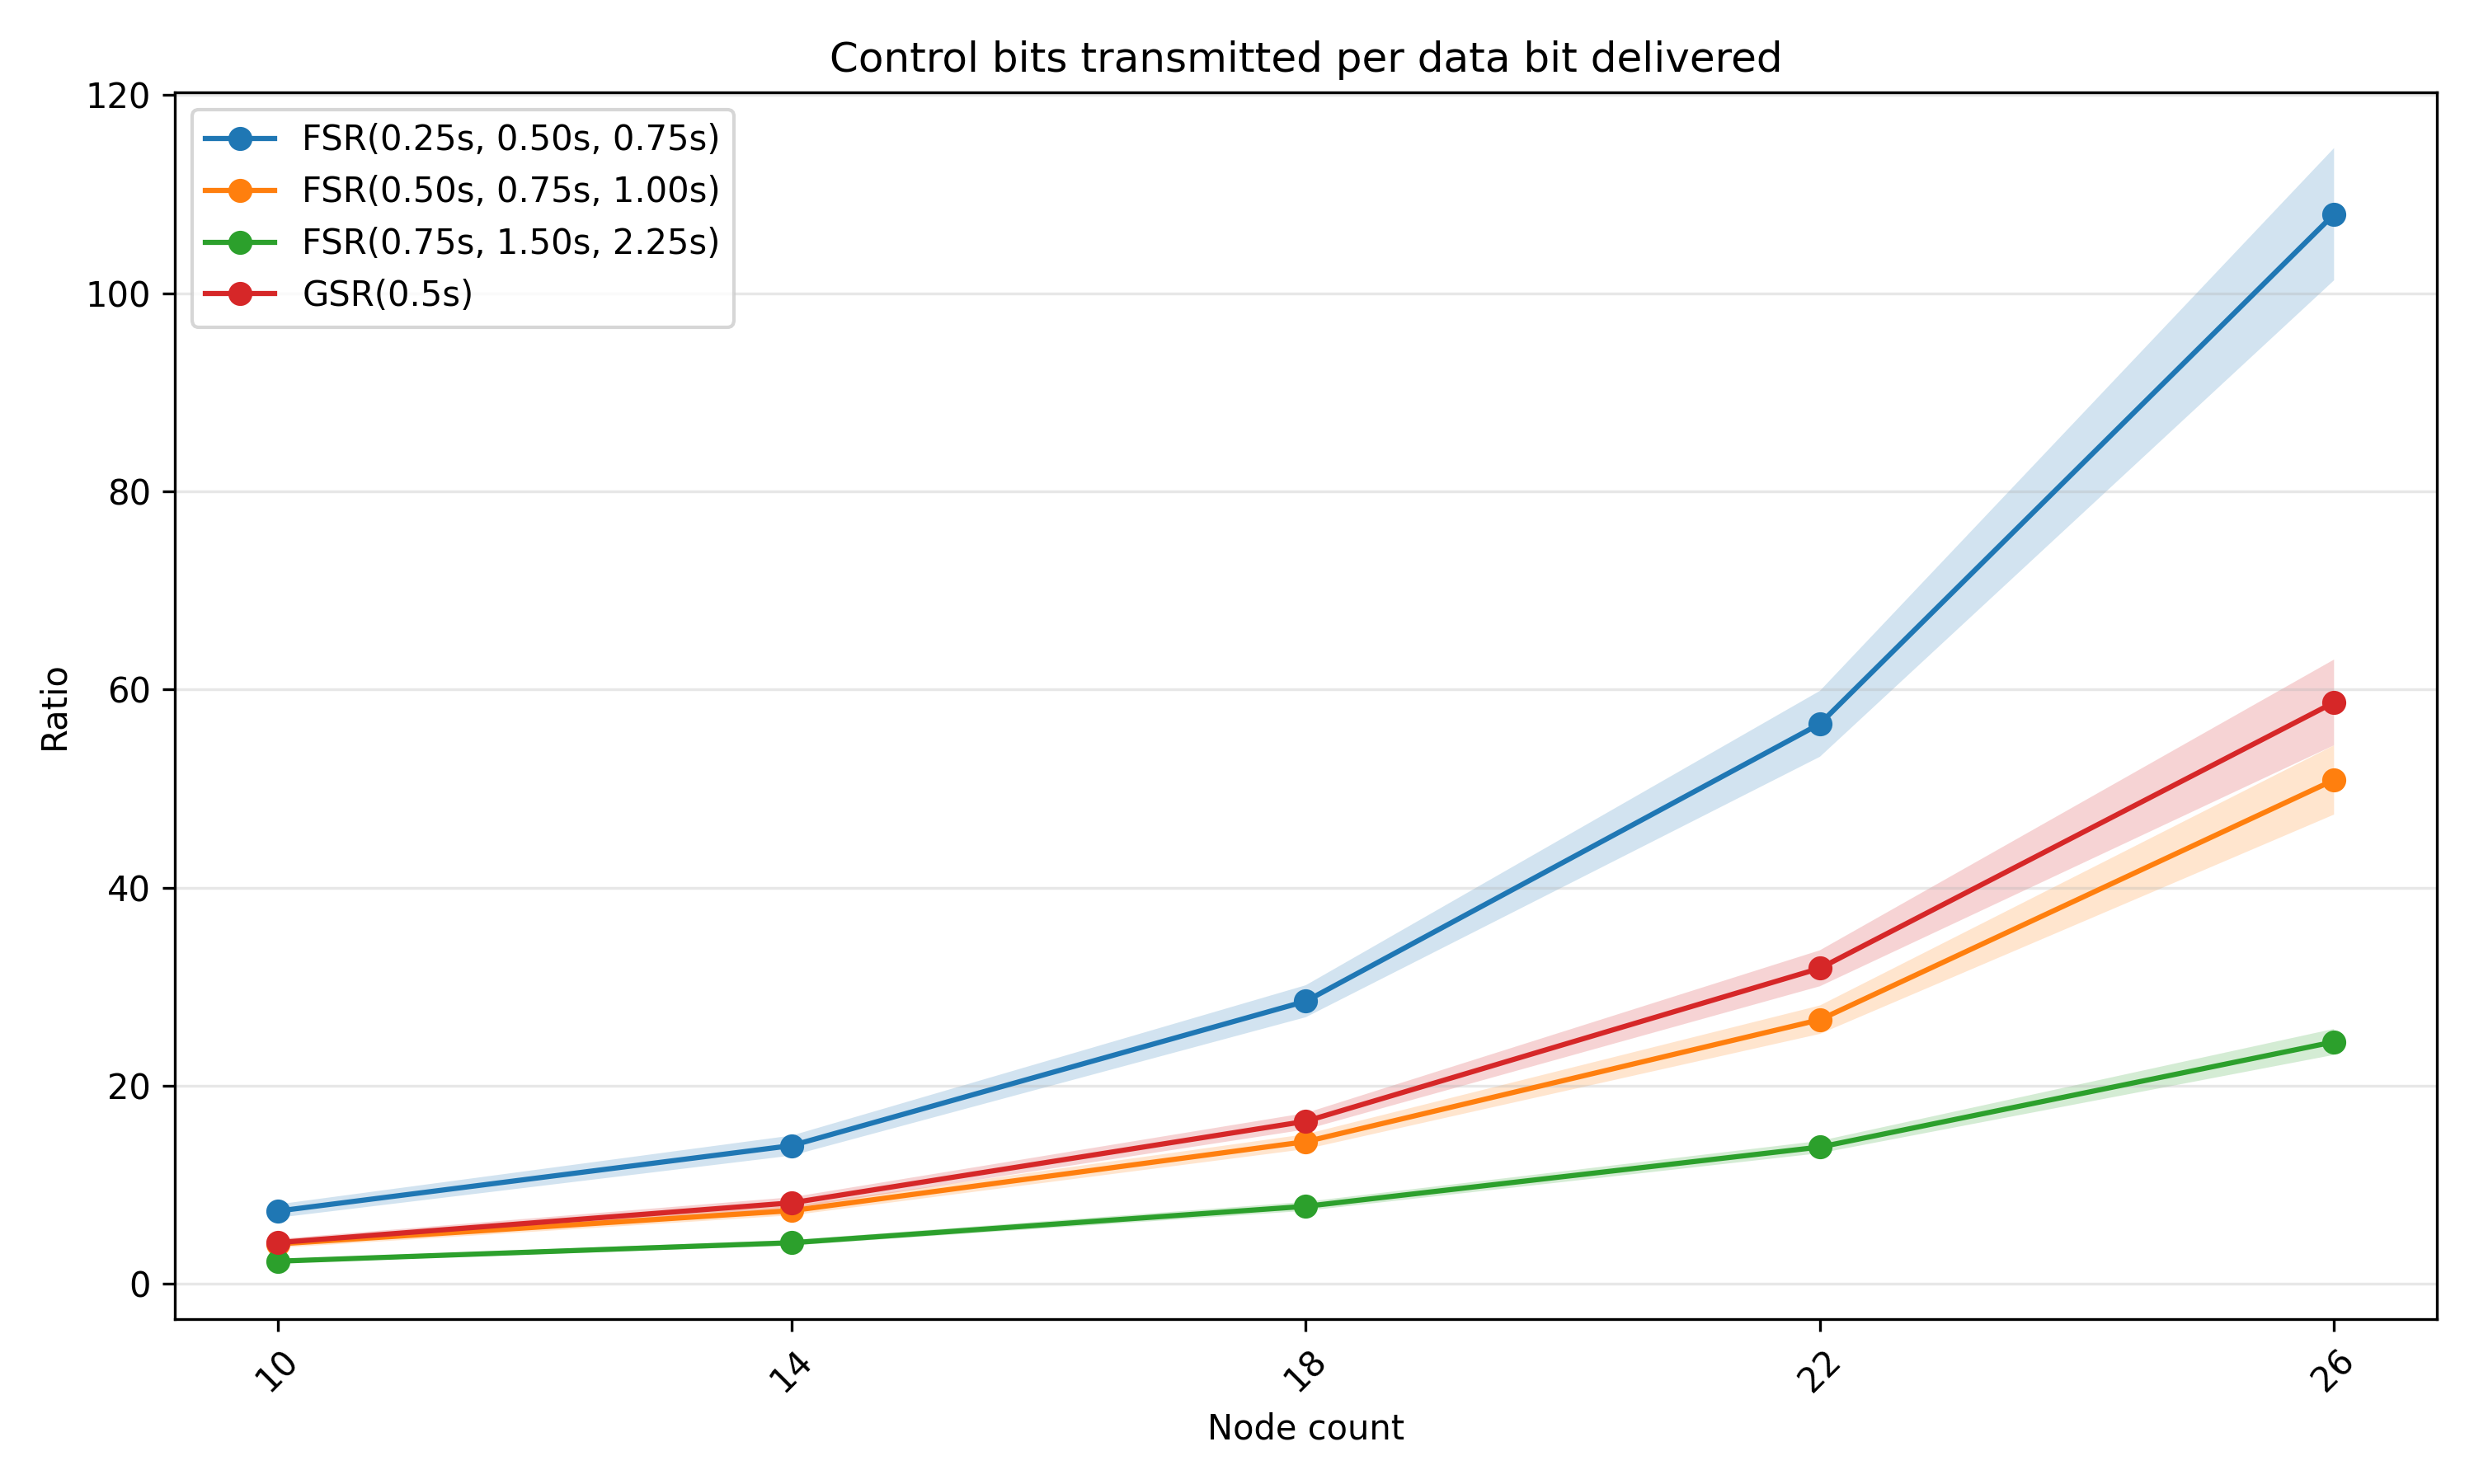
\includegraphics[width=\textwidth]{../figures/nodeCount/control_bits_transmitted_per_data_bit_delivered.png}
        \caption{Control bits transmitted per data bit delivered}
        \label{fig:control_bits_node}
    \end{subfigure}
    \caption{Node count}
    \label{fig:node}
\end{figure}

\subsubsection{Message length}
Figure \ref{fig:mlen} shows the effects of message length on the tested metrics.

Message length has a linear relationship with throughput, as shown in Figure \ref{fig:tput_mlen}. The longer the message, the more bits are transmitted, leading to higher throughput. This shows that the default link capacity of 8 Mbps is sufficient for the message lengths used in the simulation.

The effect of message length on end-to-end delay is similar to that on throughput, where larger messages lead to larger delays.

There does not seem to be a consistent trend in the packet delivery and data transmission to delivery ratios, as shown in Figures \ref{fig:delivery_mlen} and \ref{fig:data_bits_mlen}.

Low message lengths result in a higher ratio of control bits transmitted per data bit delivered, and this is expected as message length directly affects the number of data bits delivered.

\begin{figure}
    \centering
    \begin{subfigure}[b]{0.45\textwidth}
        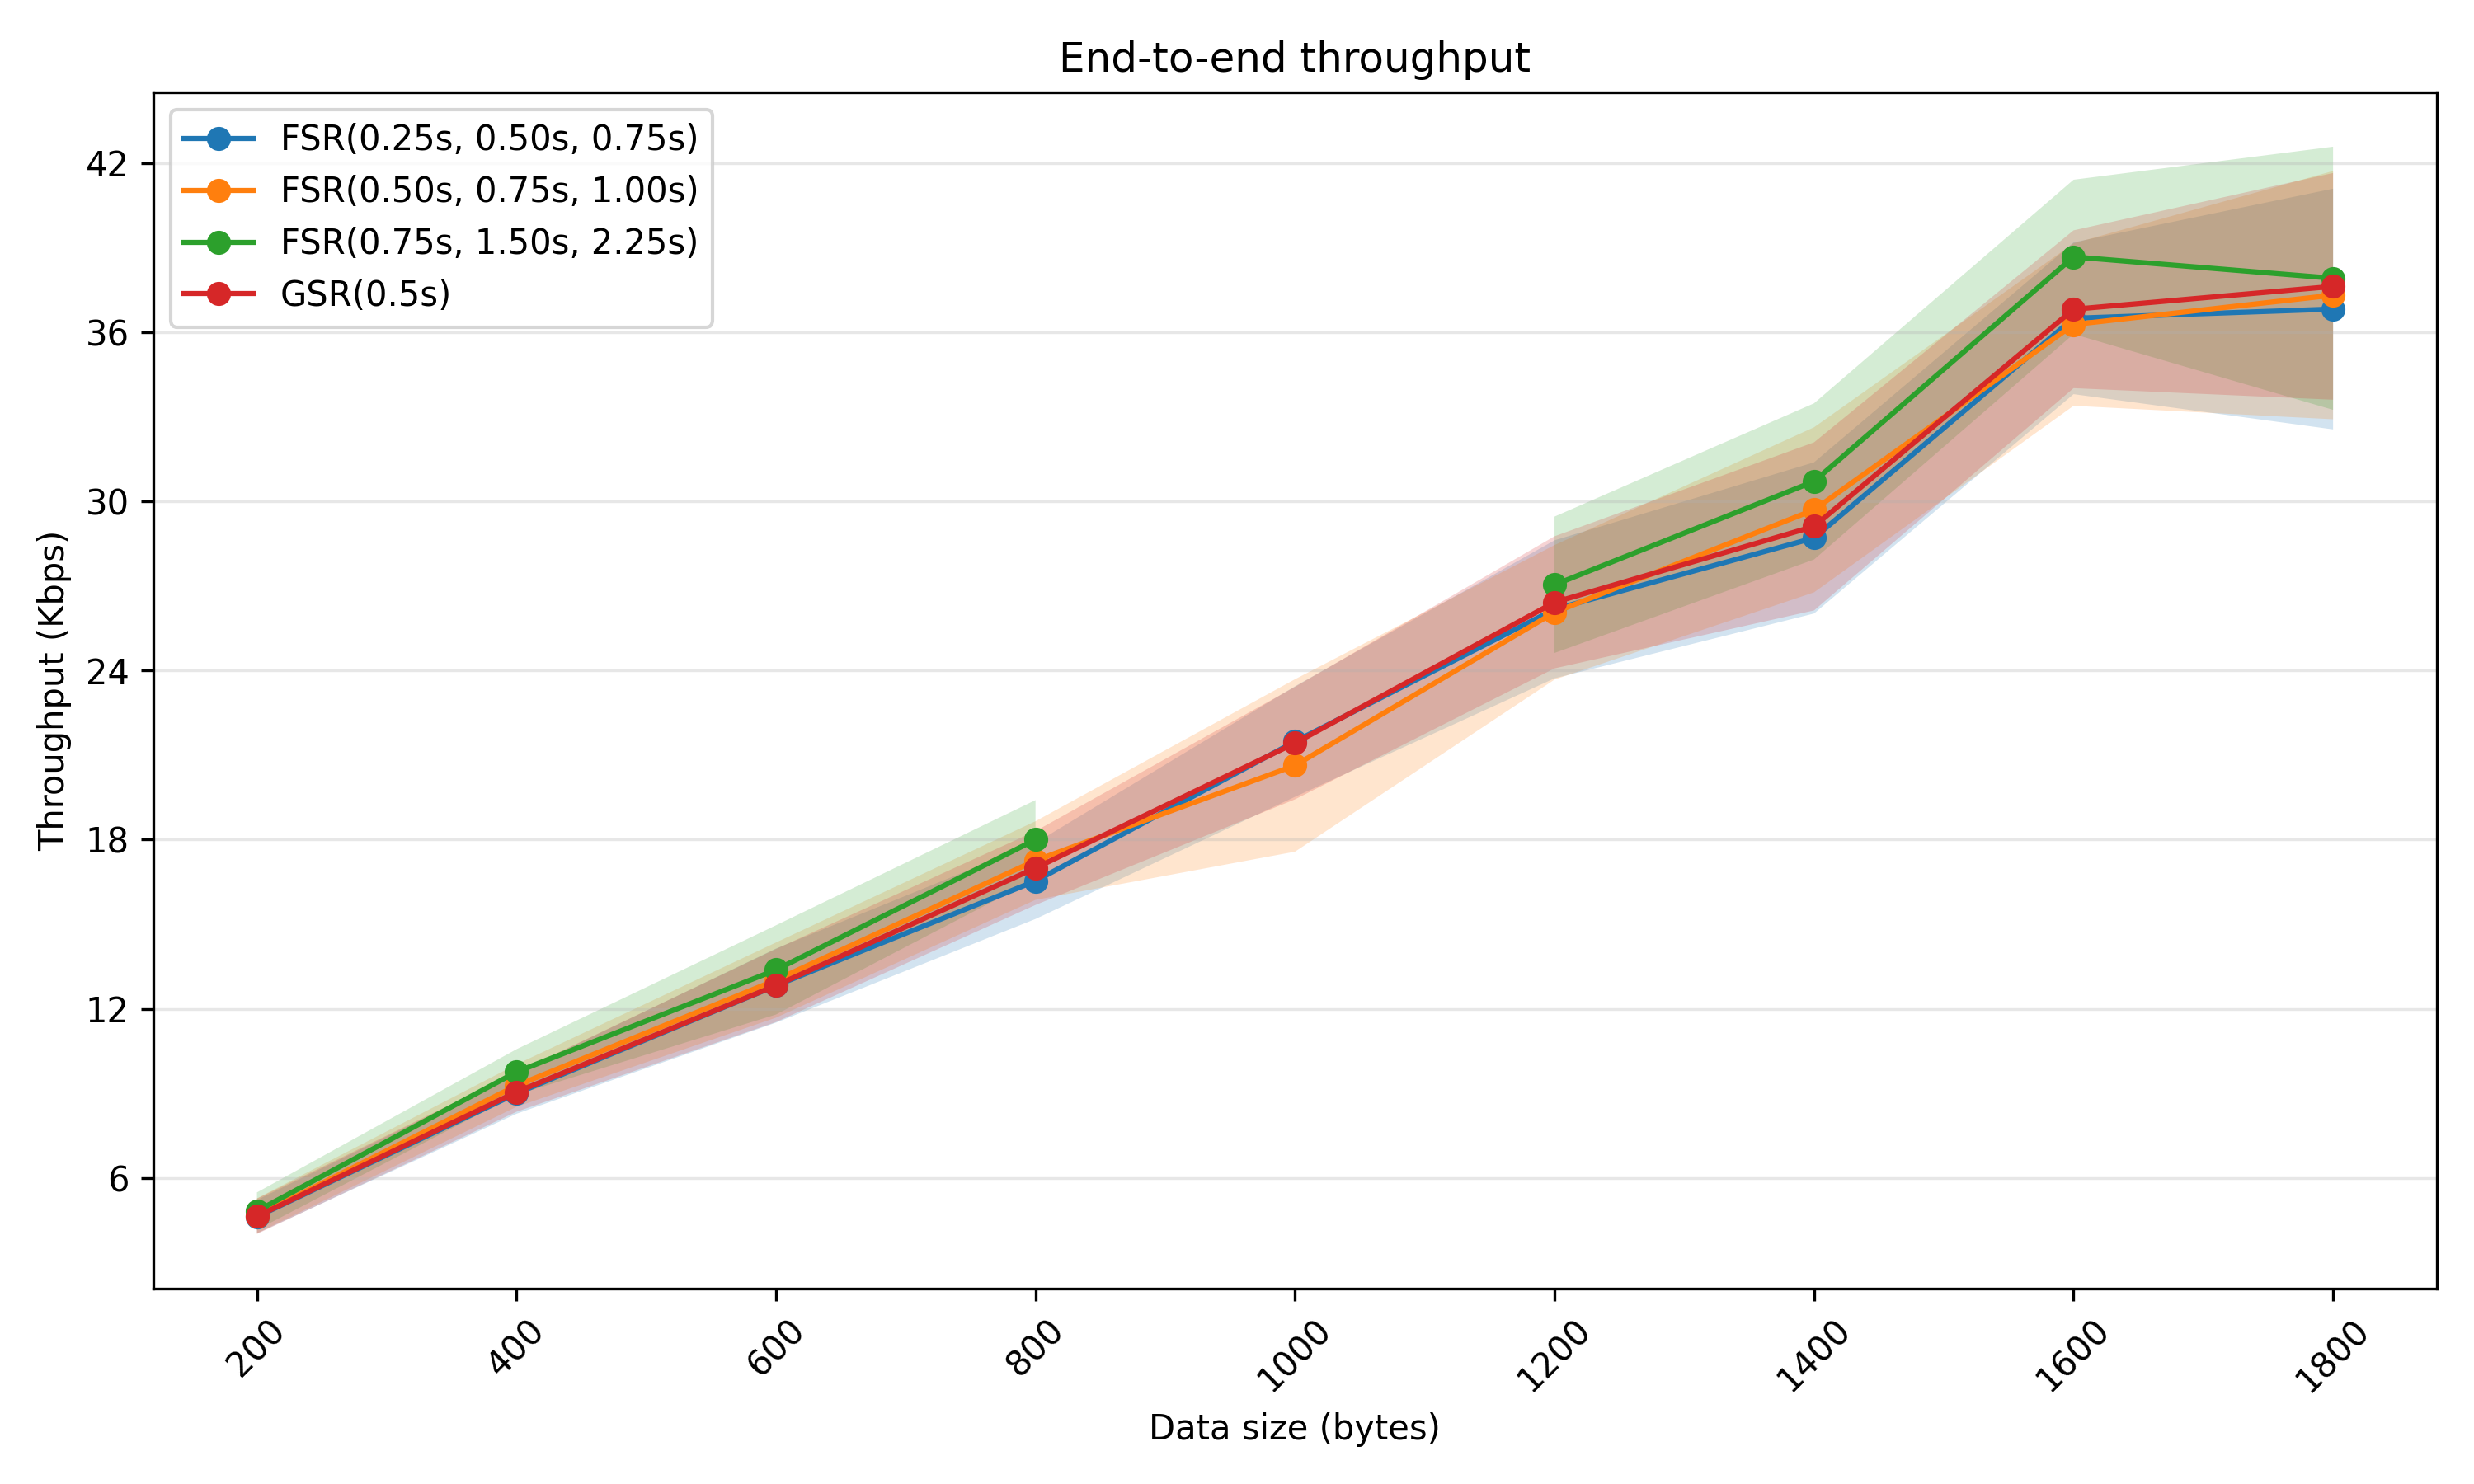
\includegraphics[width=\textwidth]{../figures/messageLength/end-to-end_throughput.png}
        \caption{End-to-end throughput}
        \label{fig:tput_mlen}
    \end{subfigure}
    \hfill
    \begin{subfigure}[b]{0.45\textwidth}
        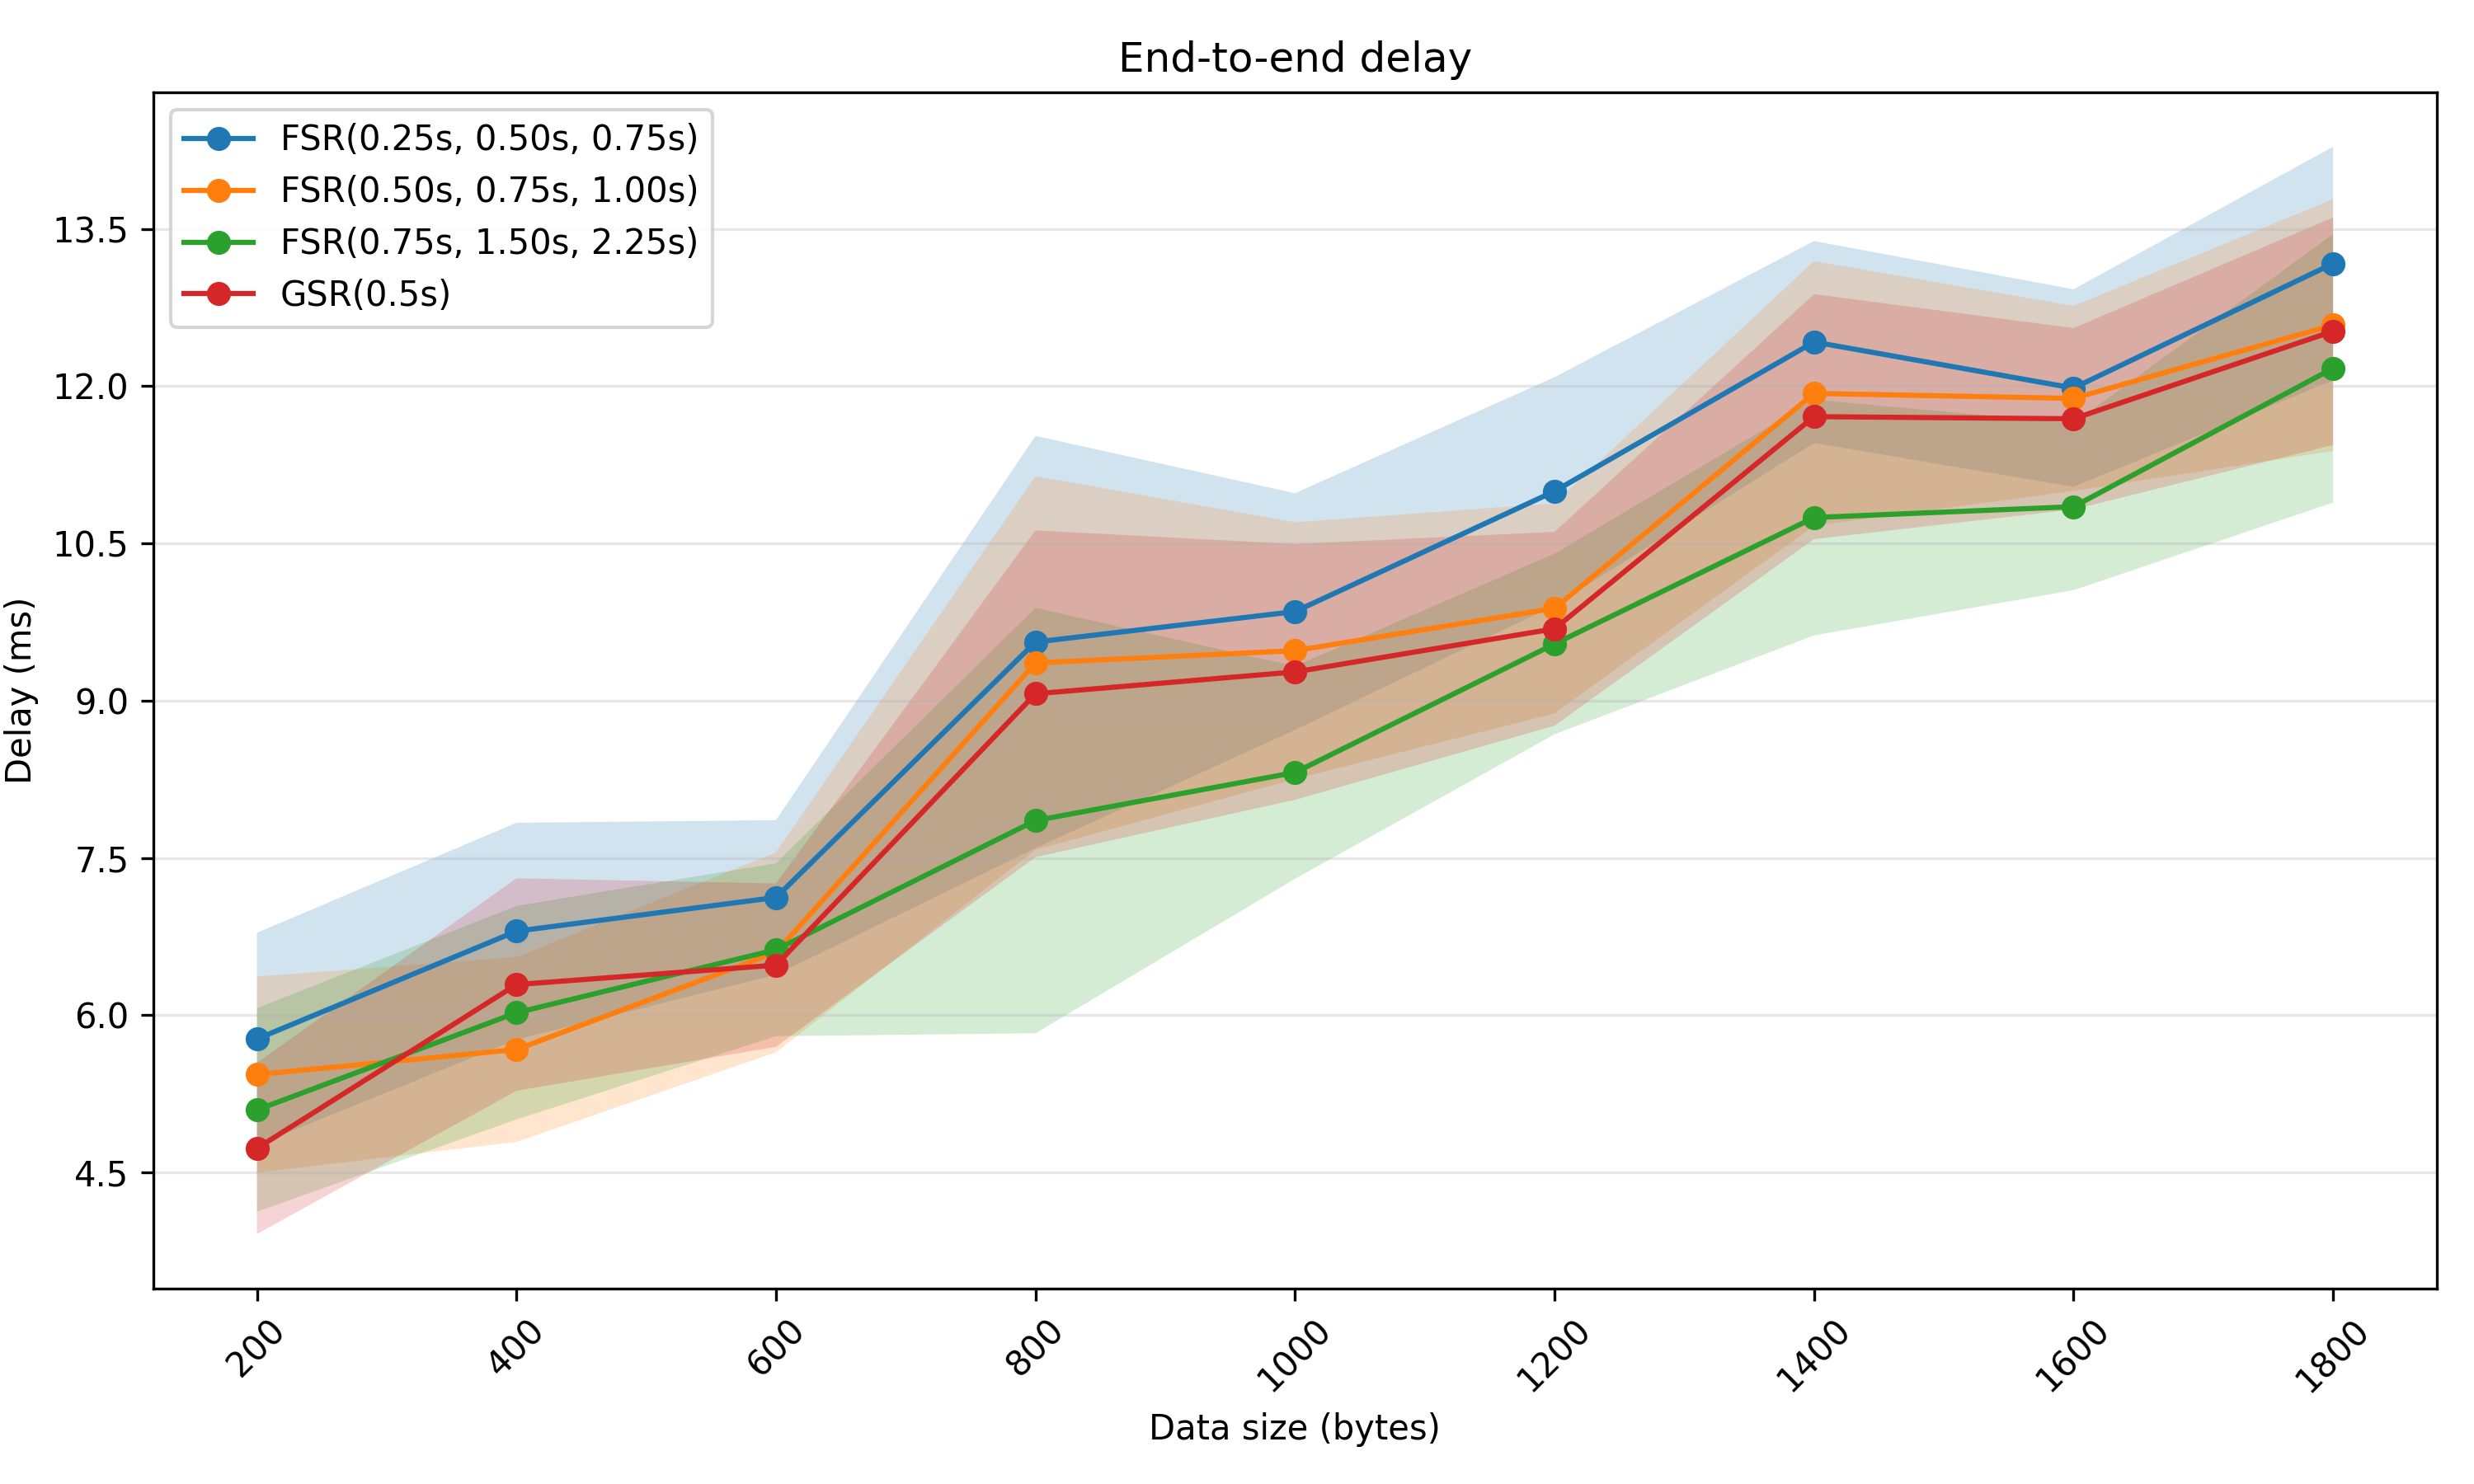
\includegraphics[width=\textwidth]{../figures/messageLength/end-to-end_delay.png}
        \caption{End-to-end delay}
        \label{fig:delay_mlen}
    \end{subfigure}
    \begin{subfigure}[b]{0.45\textwidth}
        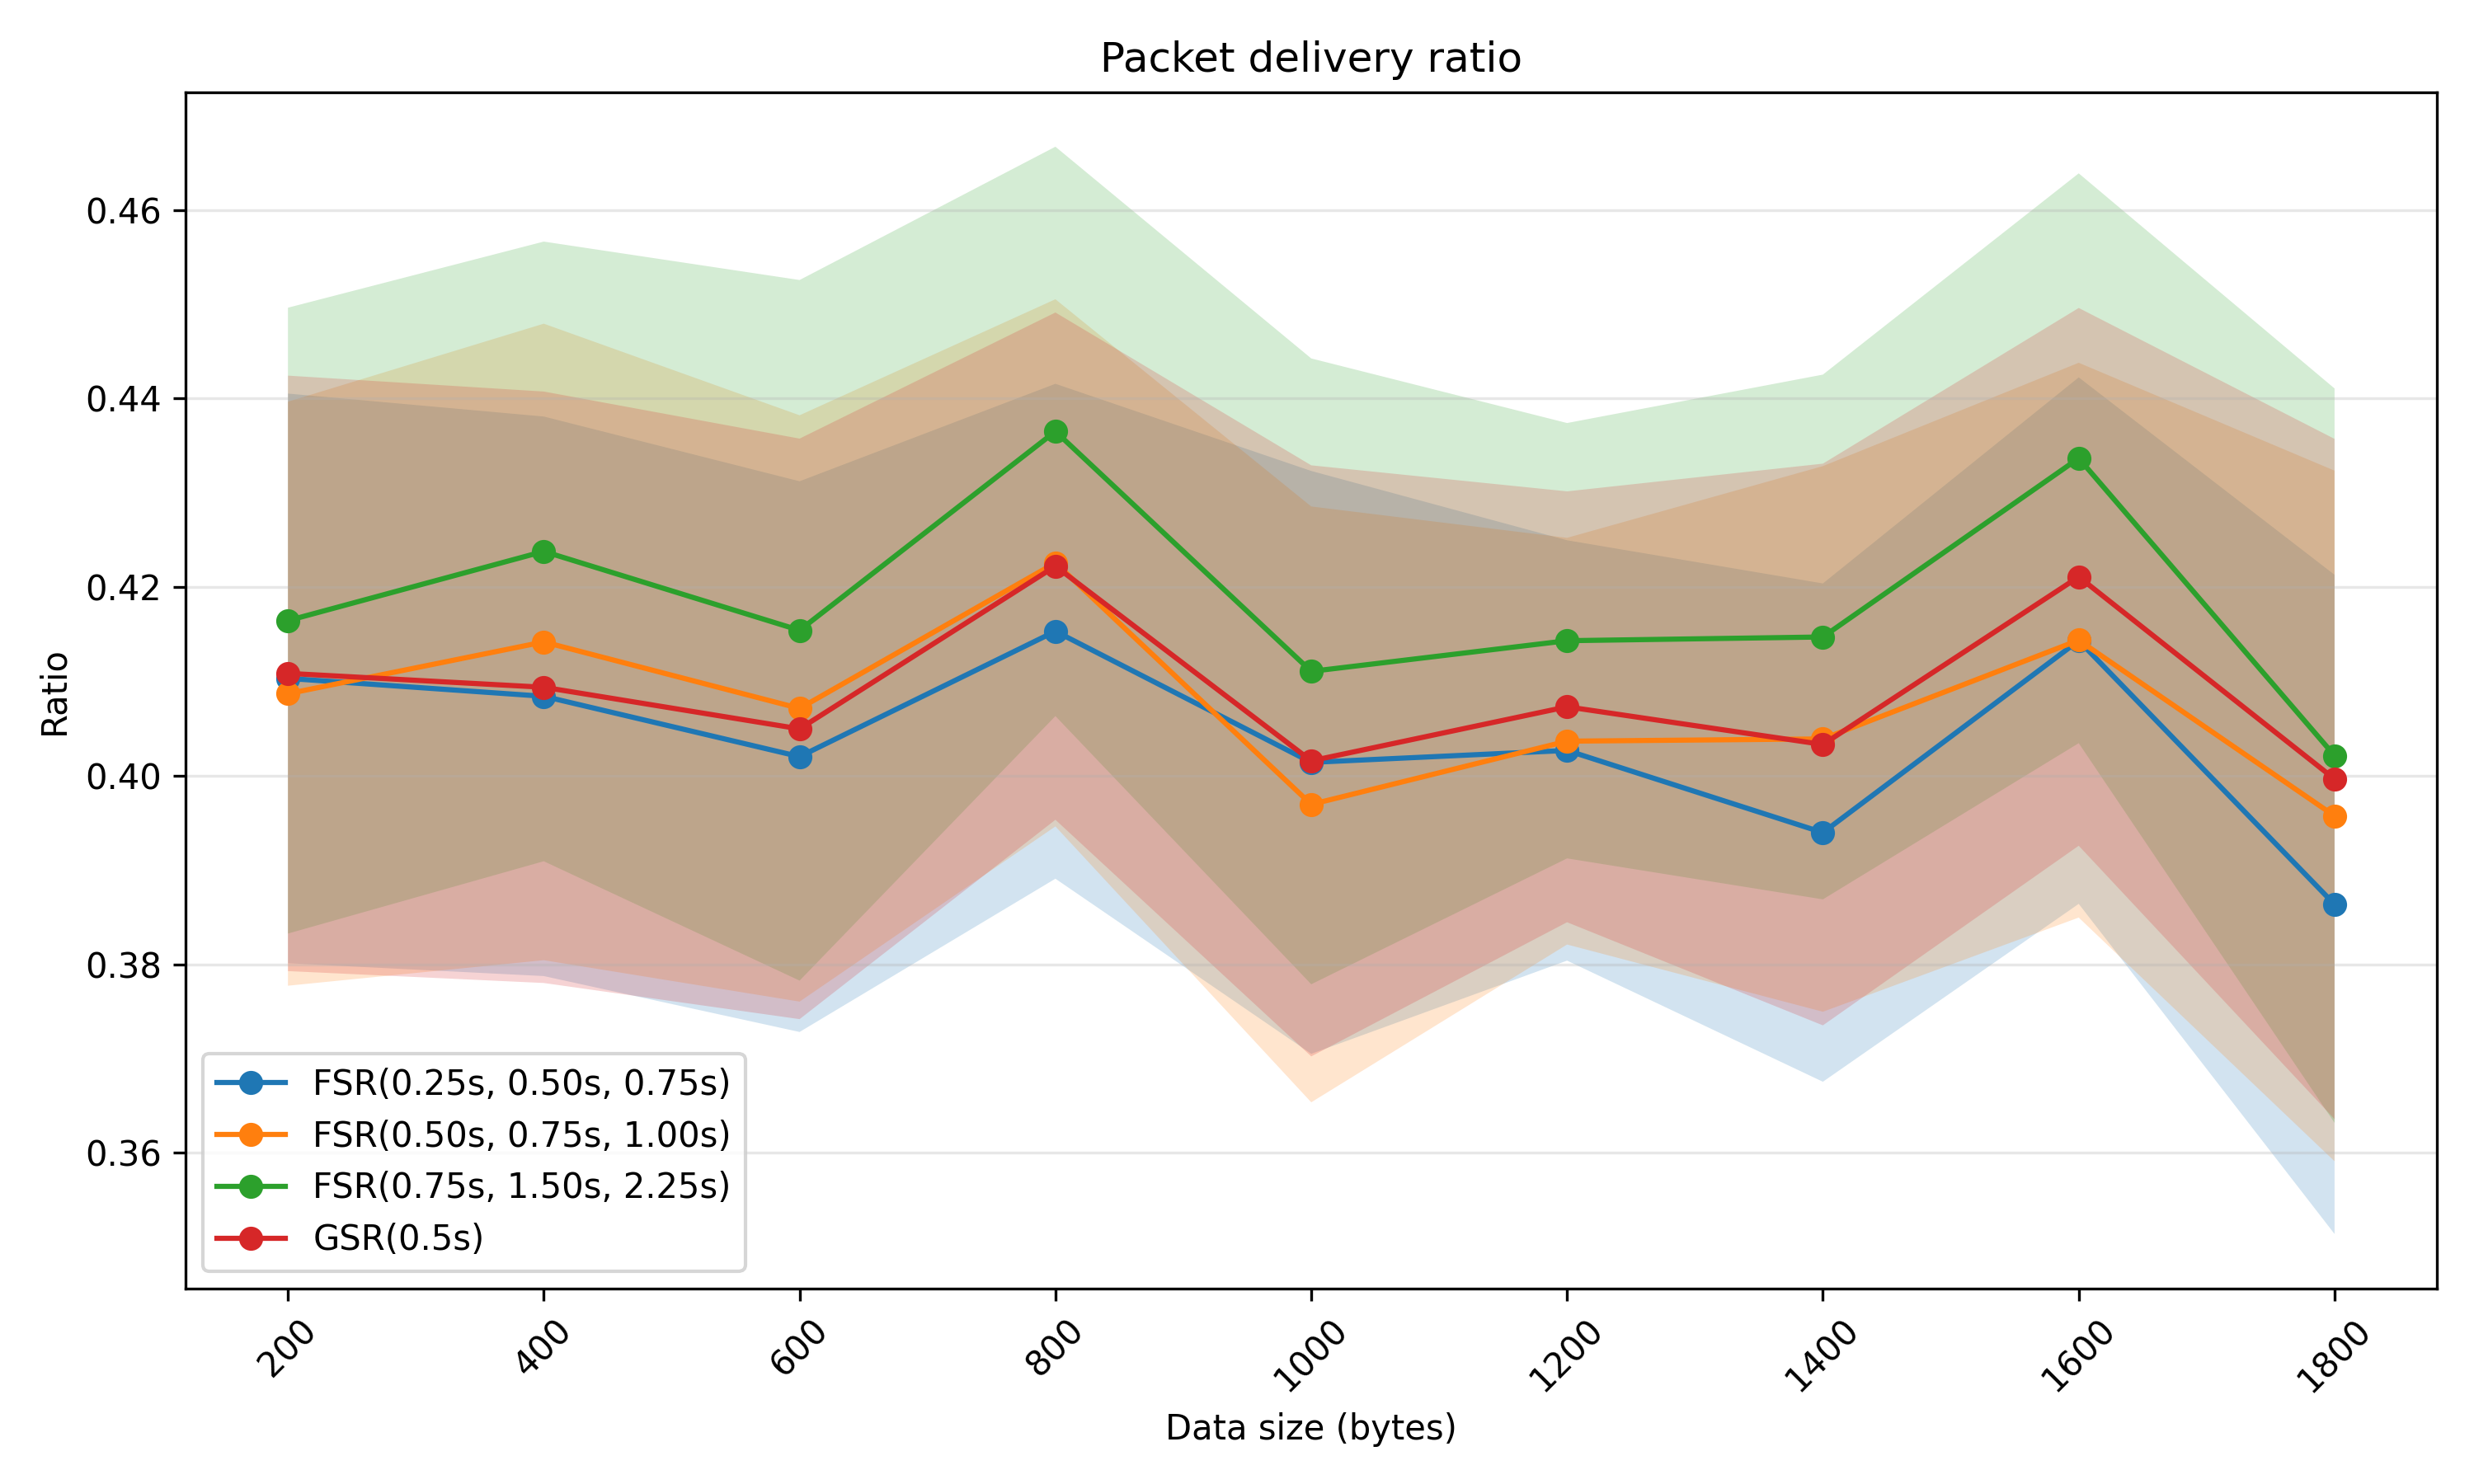
\includegraphics[width=\textwidth]{../figures/messageLength/packet_delivery_ratio.png}
        \caption{Packet delivery ratio}
        \label{fig:delivery_mlen}
    \end{subfigure}
    \begin{subfigure}[b]{0.45\textwidth}
        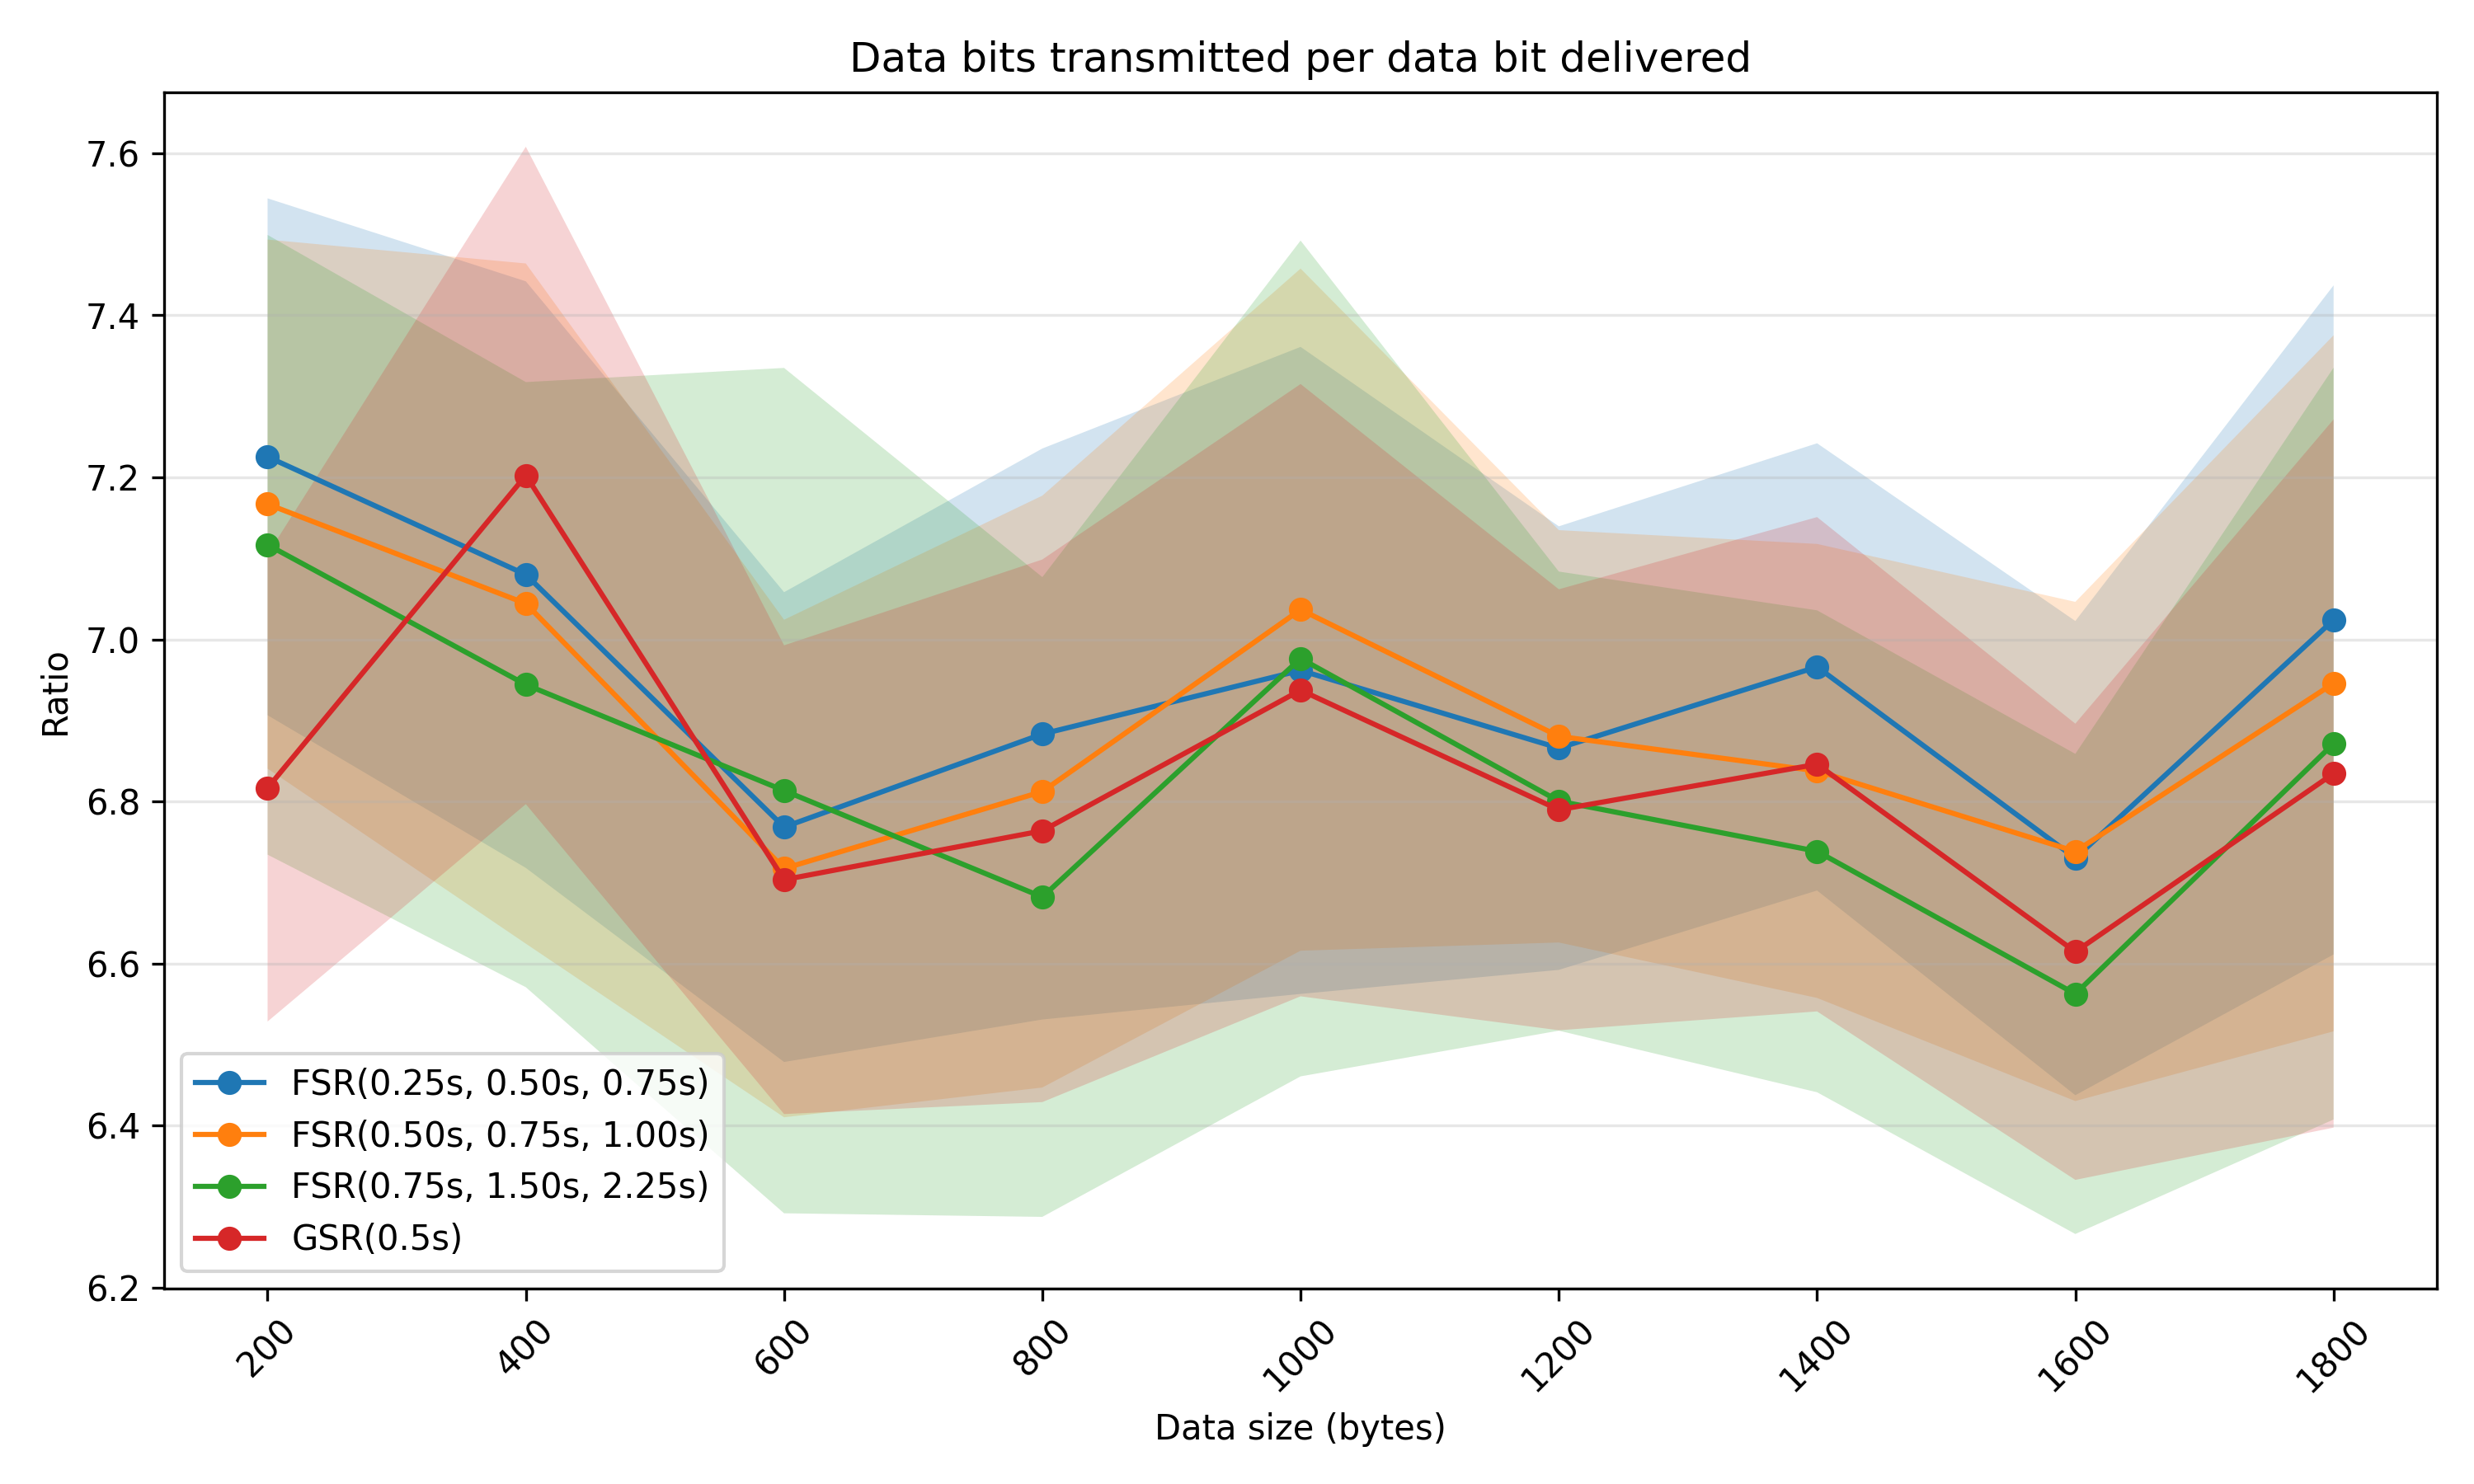
\includegraphics[width=\textwidth]{../figures/messageLength/data_bits_transmitted_per_data_bit_delivered.png}
        \caption{Data bits transmitted per data bit delivered}
        \label{fig:data_bits_mlen}
    \end{subfigure}
    \begin{subfigure}[b]{0.45\textwidth}
        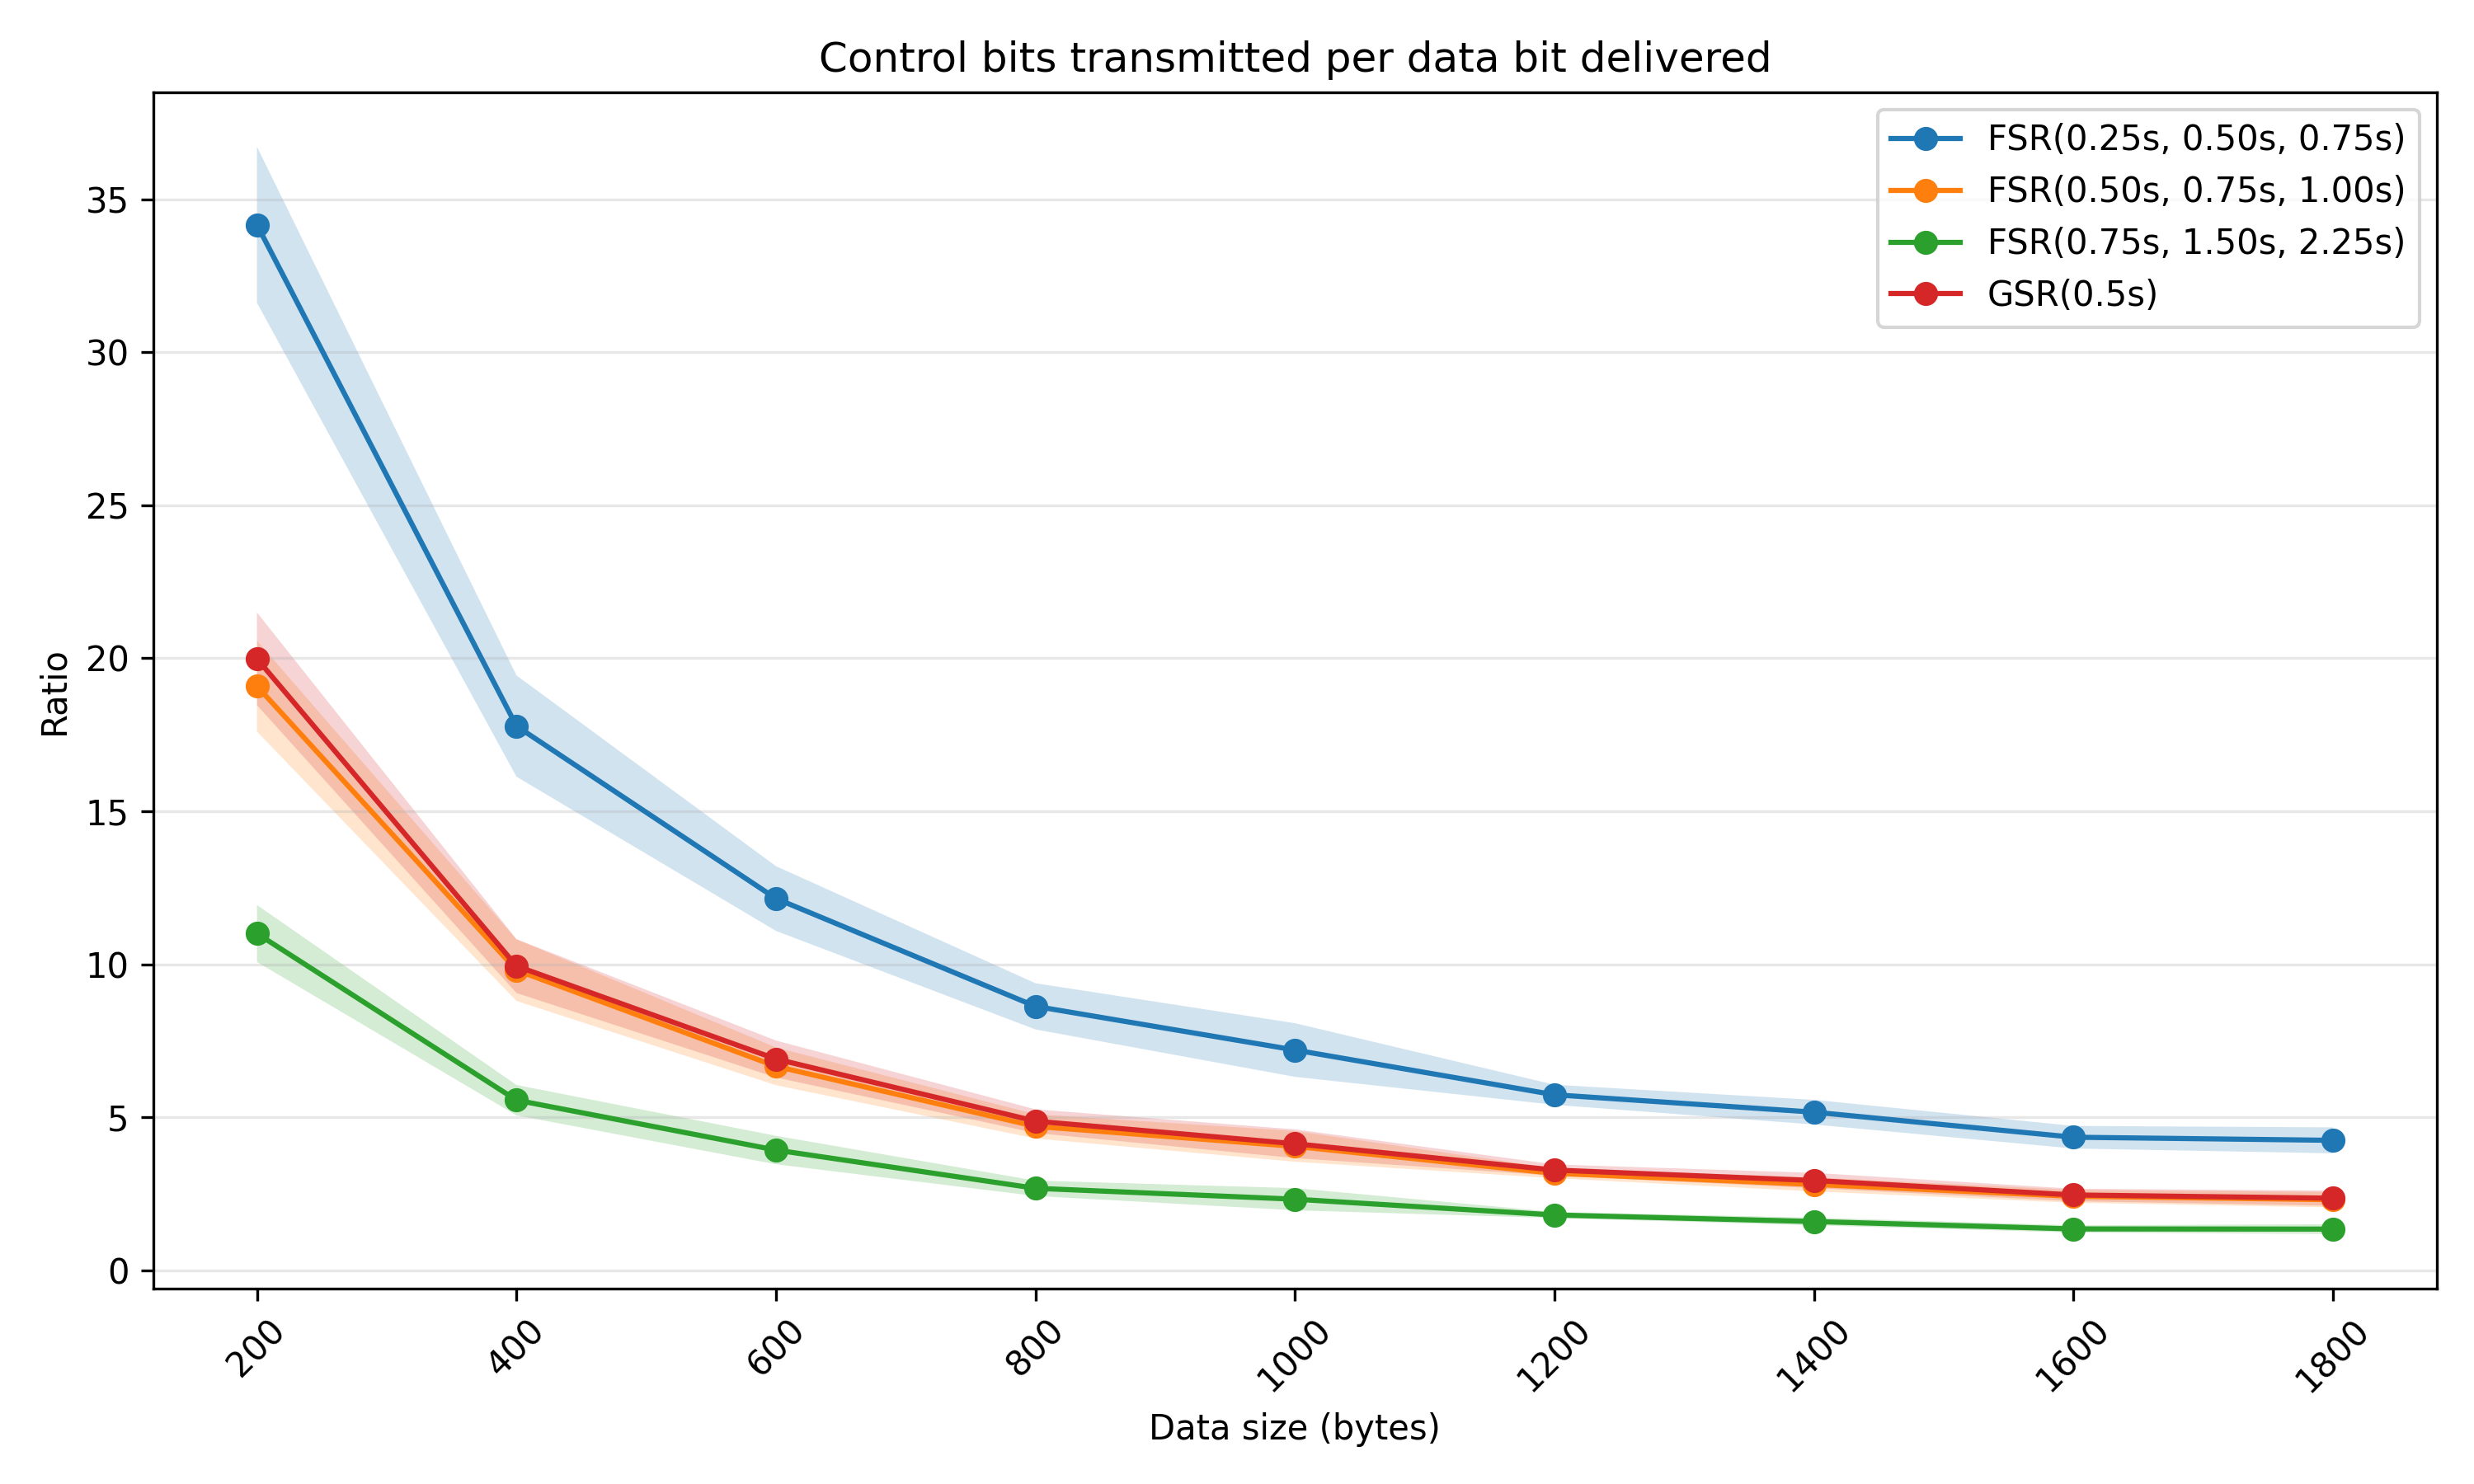
\includegraphics[width=\textwidth]{../figures/messageLength/control_bits_transmitted_per_data_bit_delivered.png}
        \caption{Control bits transmitted per data bit delivered}
        \label{fig:control_bits_mlen}
    \end{subfigure}
    \caption{Message length}
    \label{fig:mlen}
\end{figure}

\subsubsection{Message send interval}
Figure \ref{fig:send} shows the effects of message sending interval on the tested metrics.

Figure \ref{fig:tput_send} shows the results for message sending interval. Higher intervals lead to lower throughput, although the throughput also decreased at the minimum interval tested (50ms), which is likely due to the increased contention for the shared medium, as well as messages being sent too frequently for the mobile nodes to handle efficiently.

End-to-end delay has an interesting outlier at the lowest value tested, as seen in Figure \ref{fig:delay_send}. It is likely that the higher transmission demands caused extreme traffic congestion beyond the capacity of the network, which hindered the delivery of messages. This is also visible in the packet delivery ratio and data bit transmission-to-delivery ratios in Figures \ref{fig:delivery_send} and \ref{fig:data_bits_send}.

Figure \ref{fig:control_bits_send} shows that higher data message sending intervals lead to higher control-to-data bit ratios, as higher intervals reduce the number of data bits transmitted.

\begin{figure}
    \centering
    \begin{subfigure}[b]{0.45\textwidth}
        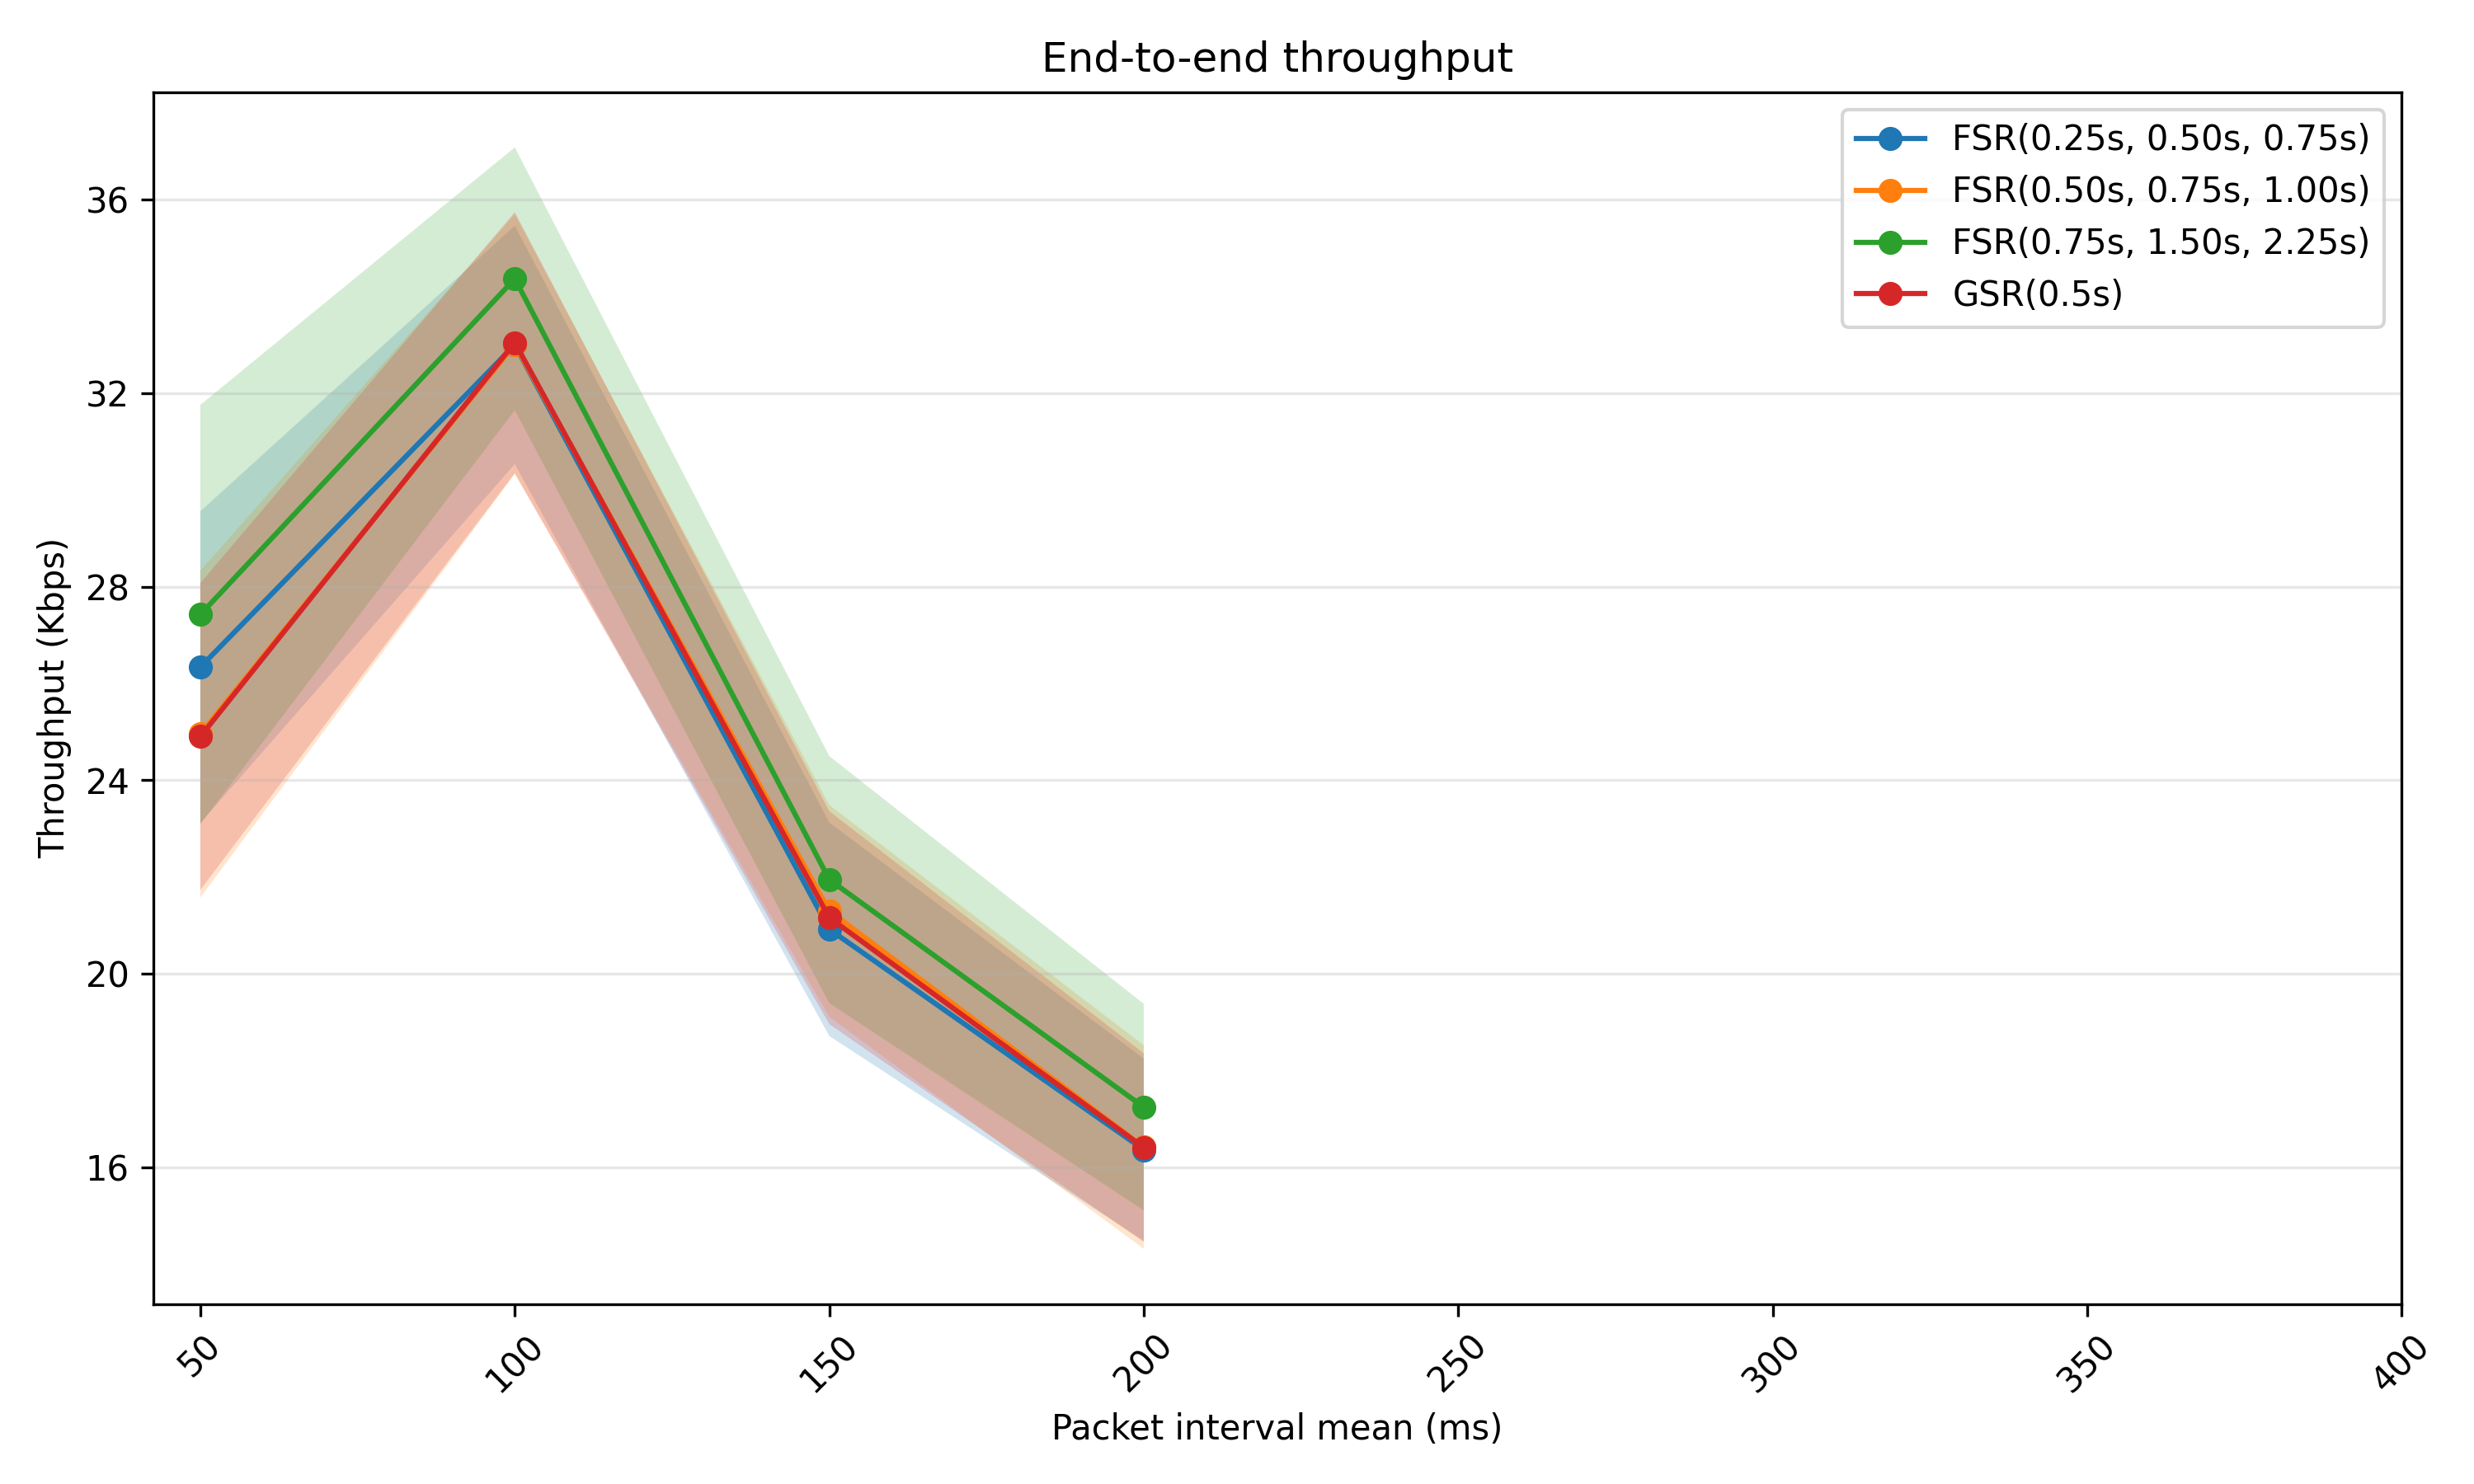
\includegraphics[width=\textwidth]{../figures/sendInterval/end-to-end_throughput.png}
        \caption{End-to-end throughput}
        \label{fig:tput_send}
    \end{subfigure}
    \begin{subfigure}[b]{0.45\textwidth}
        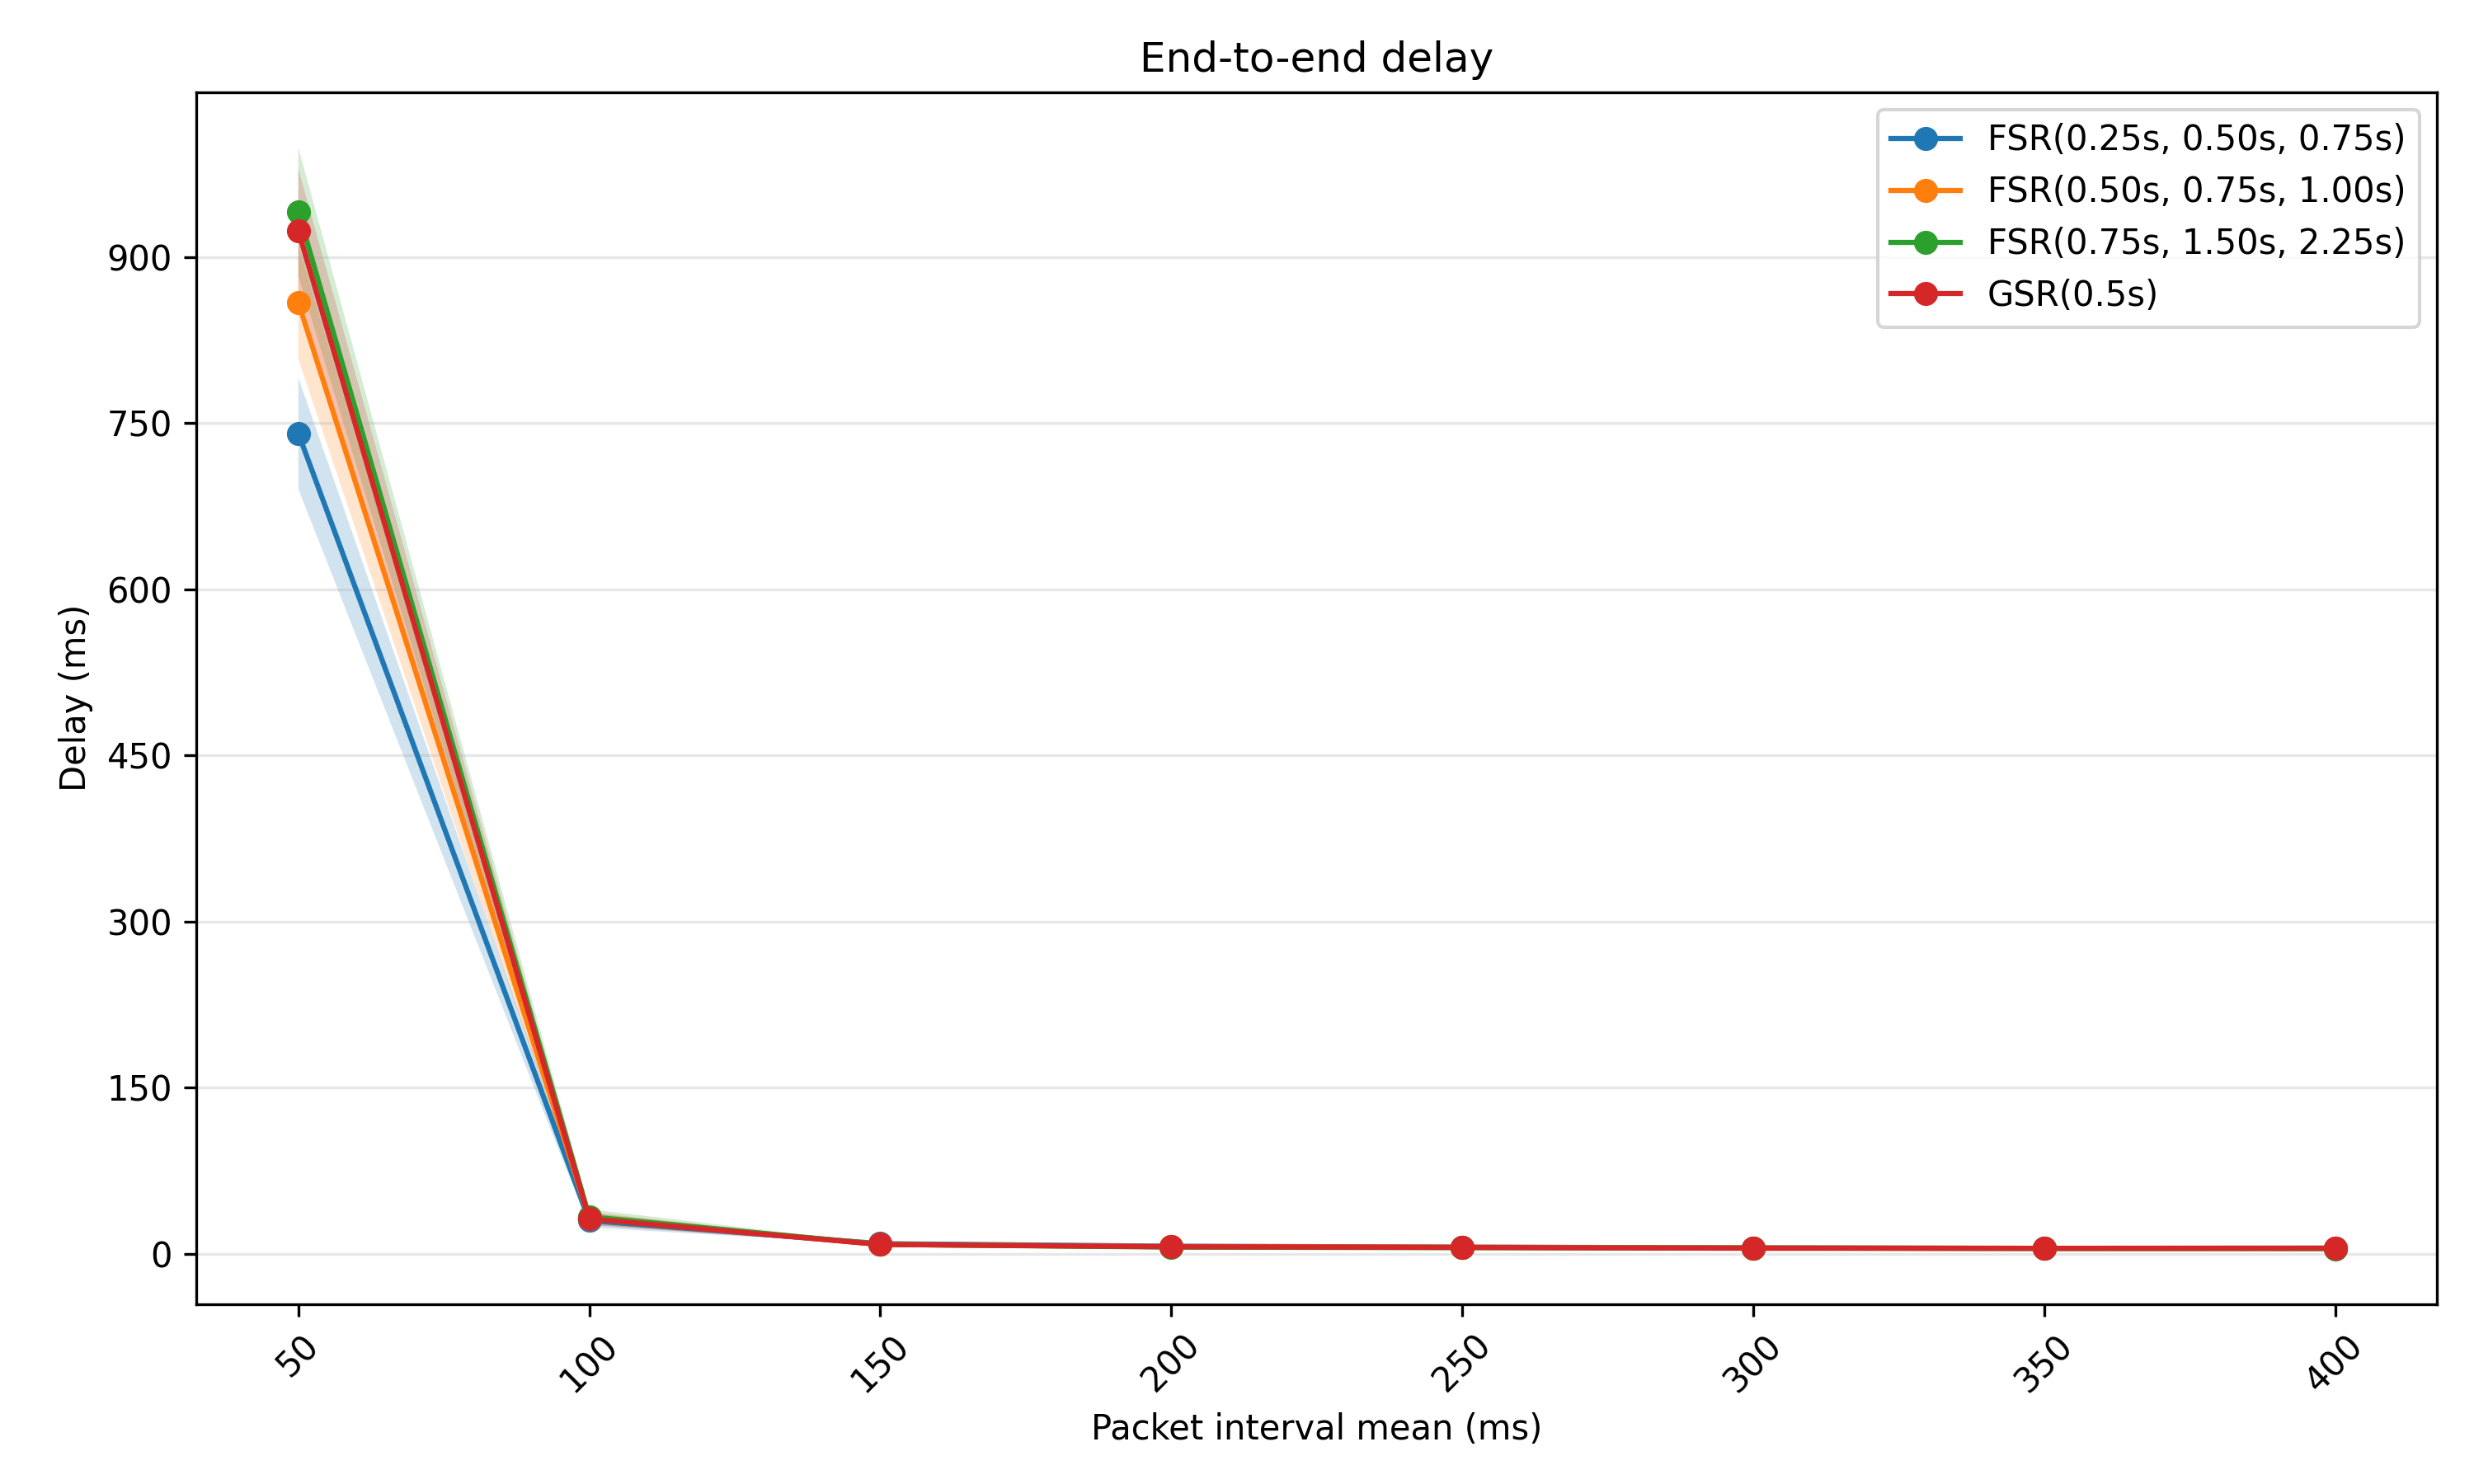
\includegraphics[width=\textwidth]{../figures/sendInterval/end-to-end_delay.png}
        \caption{End-to-end delay}
        \label{fig:delay_send}
    \end{subfigure}
    \begin{subfigure}[b]{0.45\textwidth}
        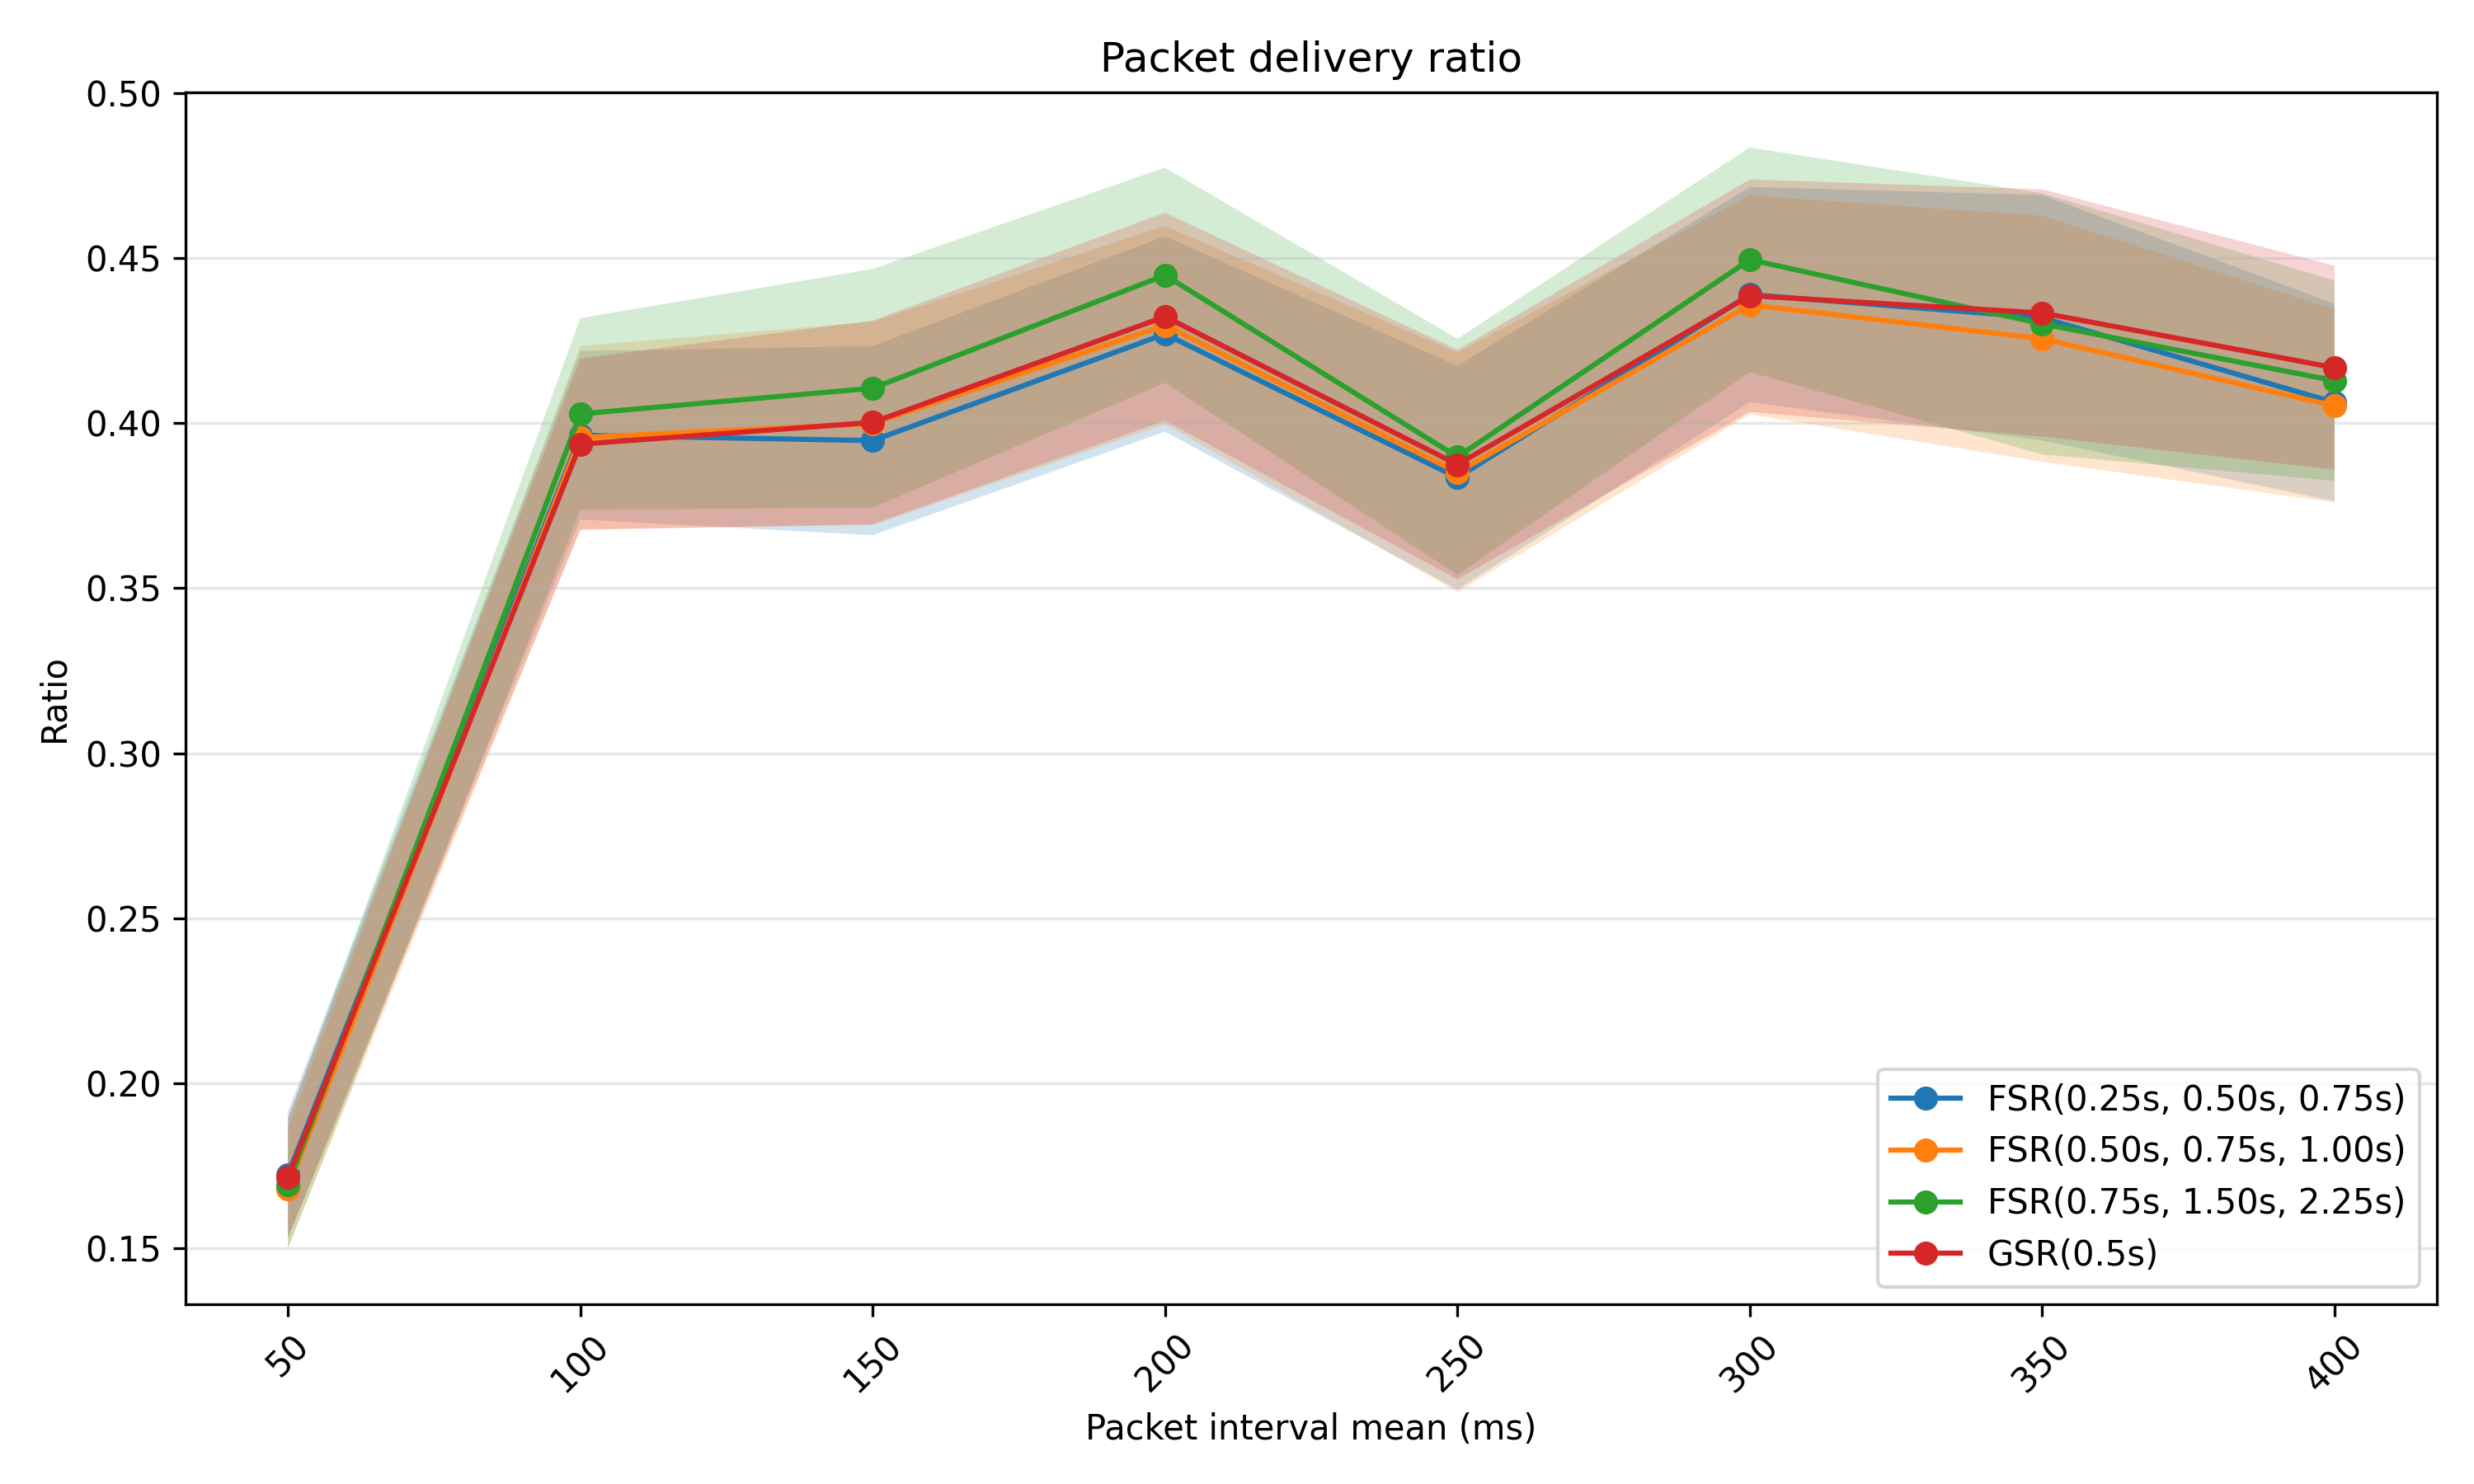
\includegraphics[width=\textwidth]{../figures/sendInterval/packet_delivery_ratio.png}
        \caption{Packet delivery ratio}
        \label{fig:delivery_send}
    \end{subfigure}
    \begin{subfigure}[b]{0.45\textwidth}
        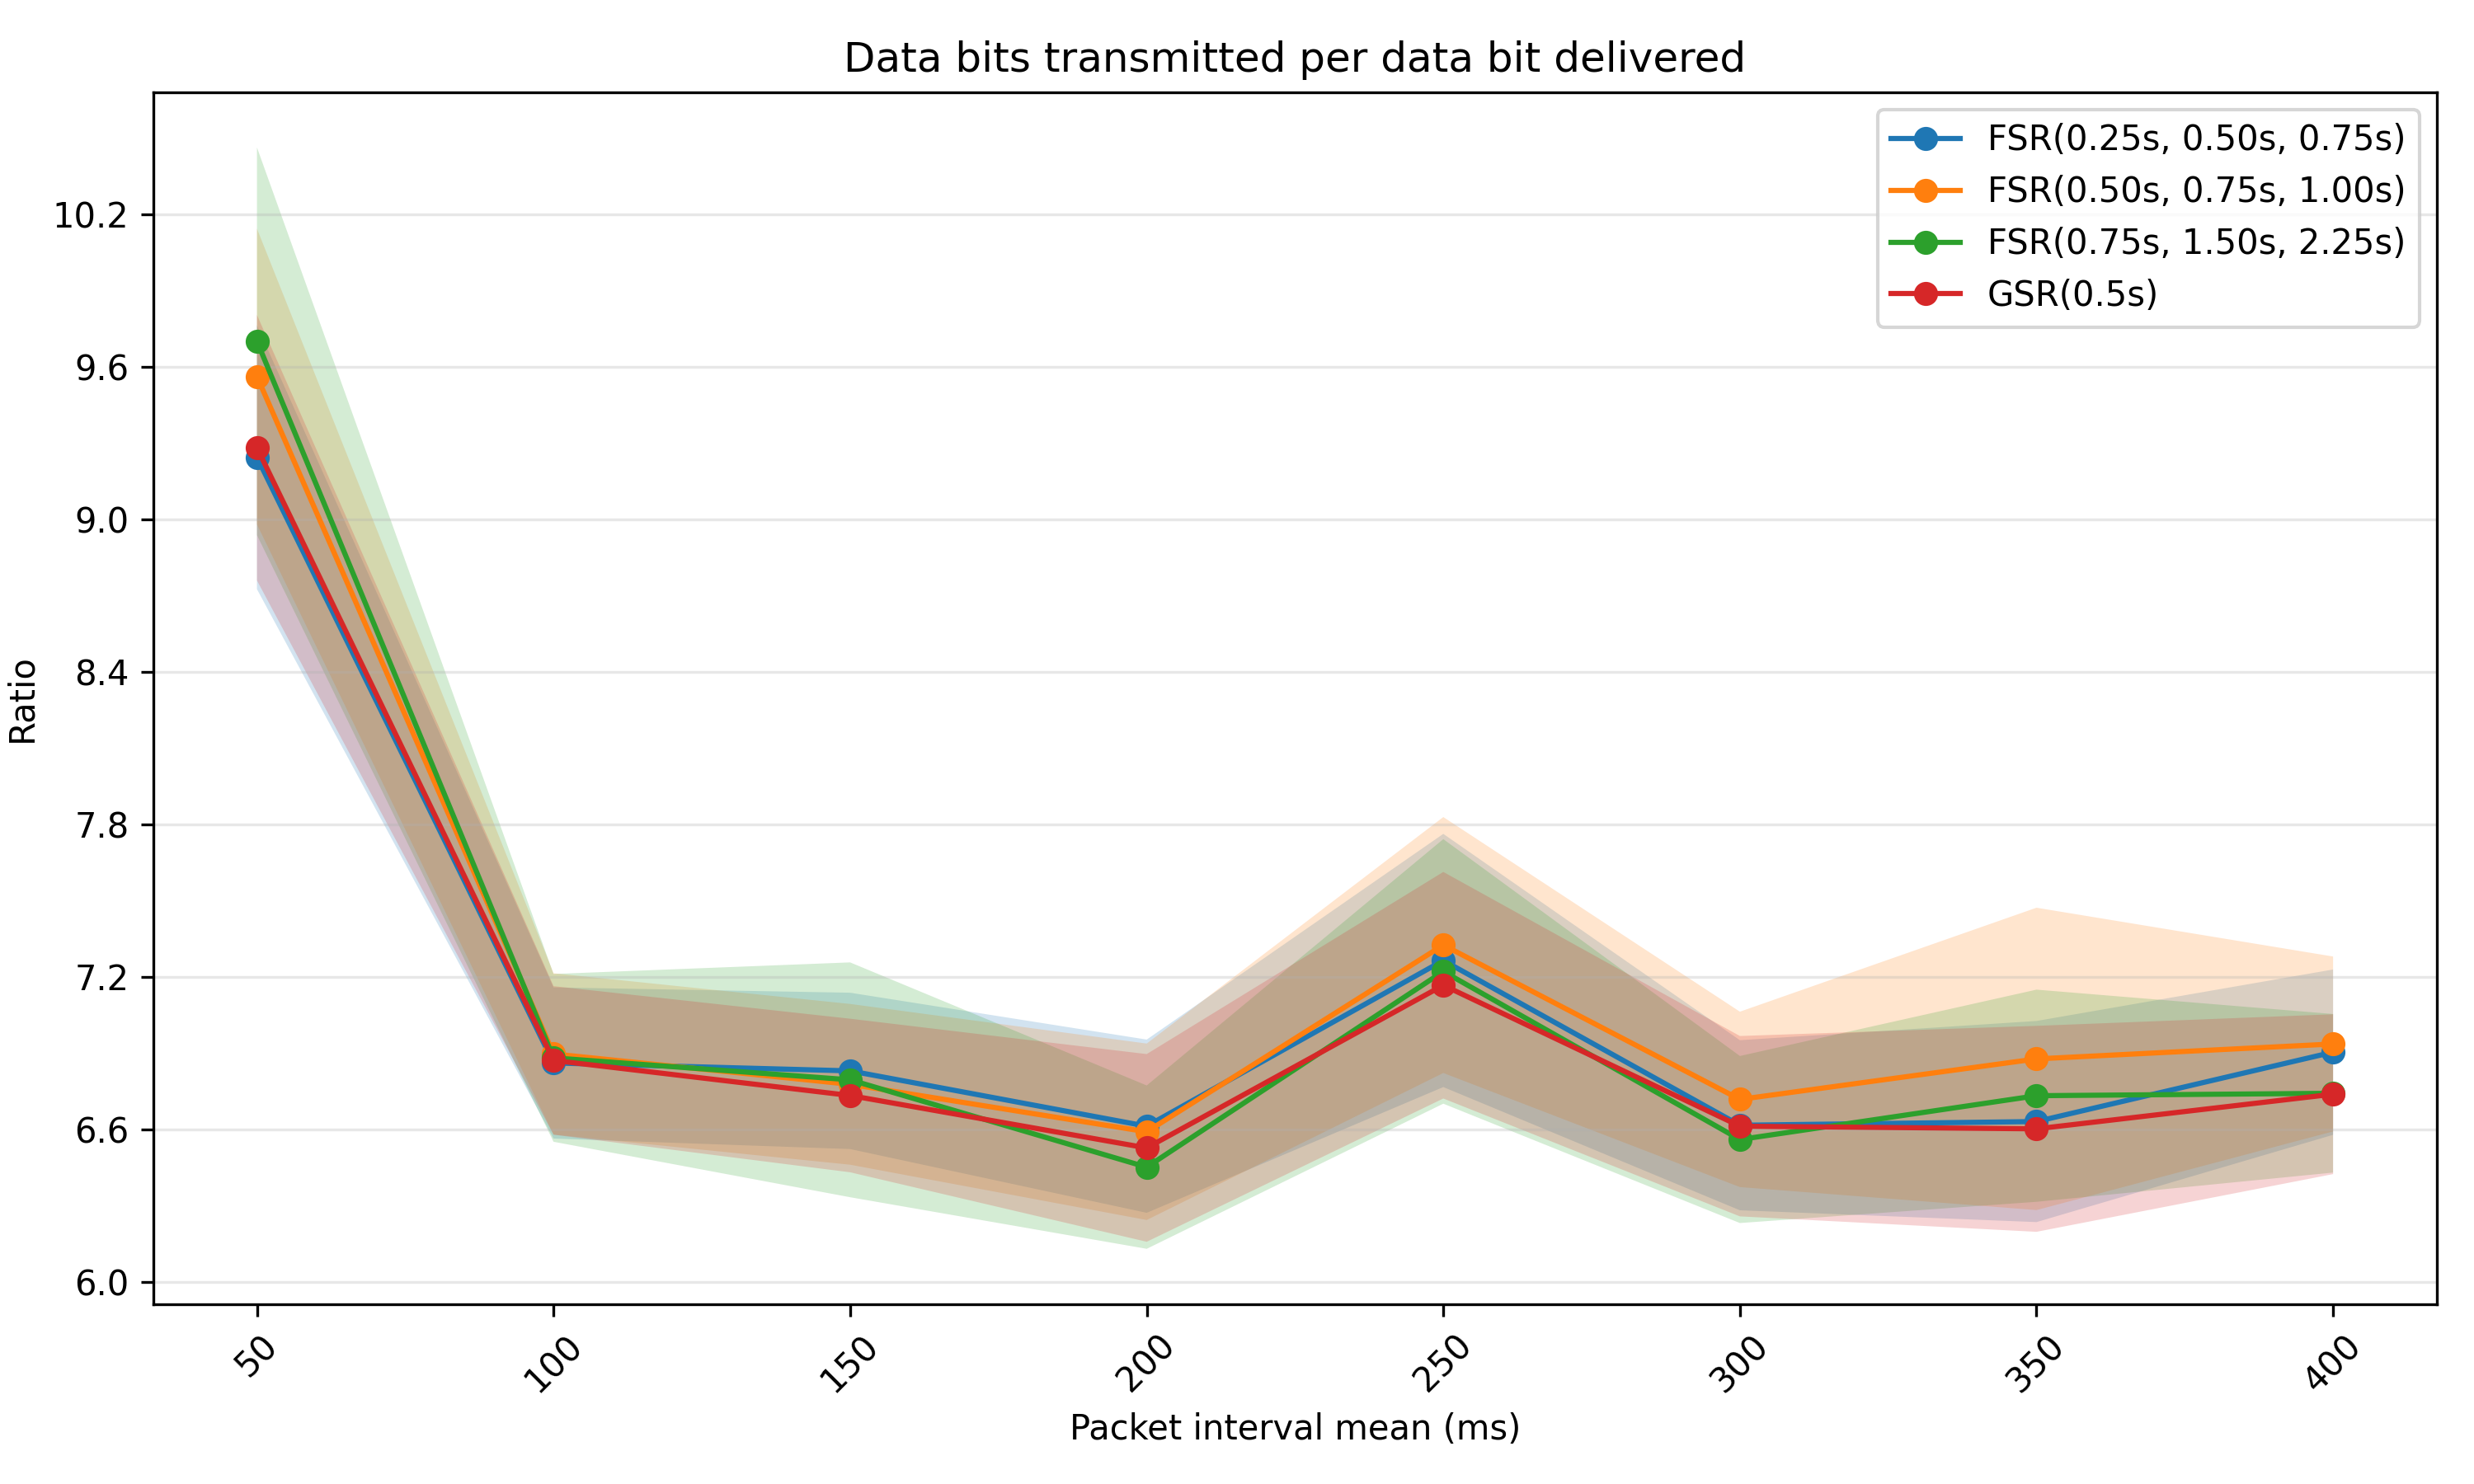
\includegraphics[width=\textwidth]{../figures/sendInterval/data_bits_transmitted_per_data_bit_delivered.png}
        \caption{Data bits transmitted per data bit delivered}
        \label{fig:data_bits_send}
    \end{subfigure}
    \begin{subfigure}[b]{0.45\textwidth}
        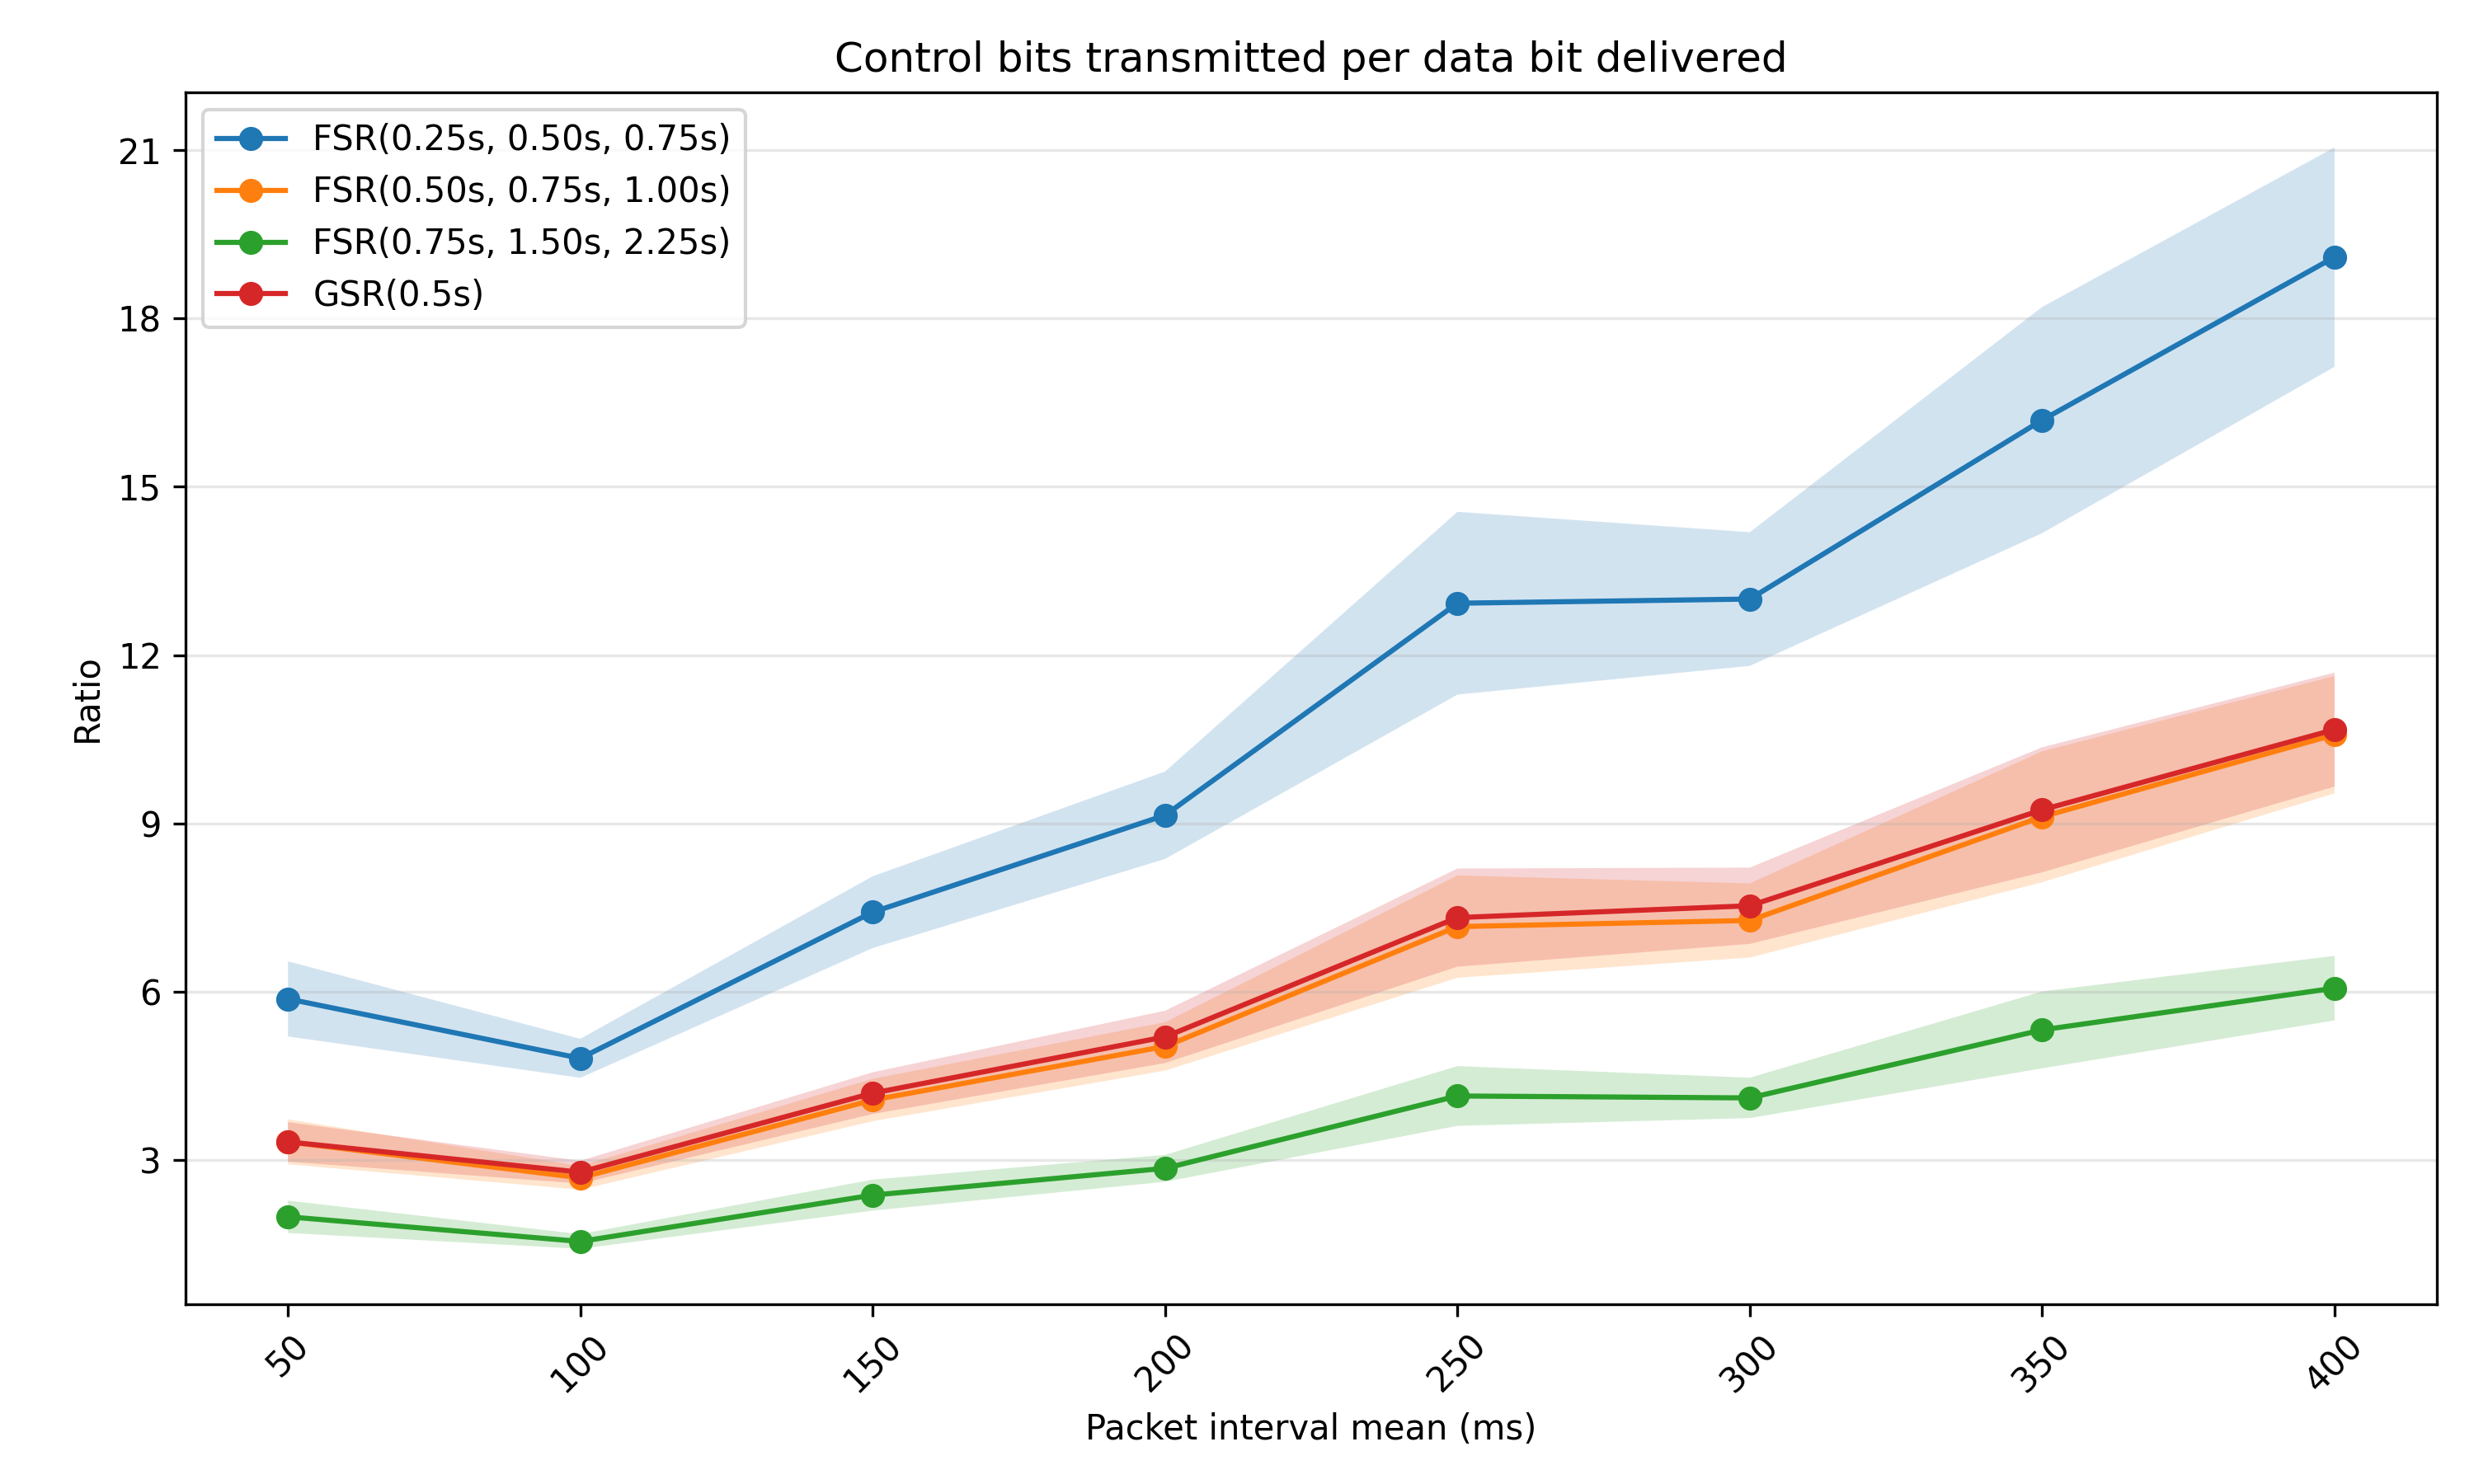
\includegraphics[width=\textwidth]{../figures/sendInterval/control_bits_transmitted_per_data_bit_delivered.png}
        \caption{Control bits transmitted per data bit delivered}
        \label{fig:control_bits_send}
    \end{subfigure}
    \caption{Mean of send interval (exponential distribution)}
    \label{fig:send}
\end{figure}


\subsubsection{Mobility speed}
Figure \ref{fig:speed} shows the effects of mobility speed on the tested metrics. The mobility values shown are the minimum speed of mobility, and the maximum speed is set to two times the minimum speed.

The effect of mobility speed on end-to-end delay is shown in Figure \ref{fig:delay_speed}. Higher mobility leads to more frequent topology changes, which leads to more changes in routes and higher delays. This is also supported by the large confidence intervals, showing the effect of random mobility in the simulation replications.

Figure \ref{fig:delivery_speed} shows that the packet delivery ratio decreases with higher mobility speeds. This is due to the increased likelihood of nodes moving out of range of each other, leading to more route changes and fewer successful transmissions. What is interesting here is that even with higher mobility, the FSR configuration with the lowest scope refresh rate still performed better than the others on average. 

The data and control bit transmission ratios are larger for higher mobility speeds, as shown in Figures \ref{fig:data_bits_speed} and \ref{fig:control_bits_speed}. As expected, higher mobility results in more topological and routing changes, resulting in less data packets delivered per transmission. For the control-to-data ratio, the effect of mobility speed is less pronounced for configurations with lower scope refresh rates.

It was difficult to measure throughput for different mobility speeds due to some instabilities in the throughput calculation in the UDP app module. For that reason those results are omitted.

\begin{figure}
    \centering
    \begin{subfigure}[b]{0.45\textwidth}
        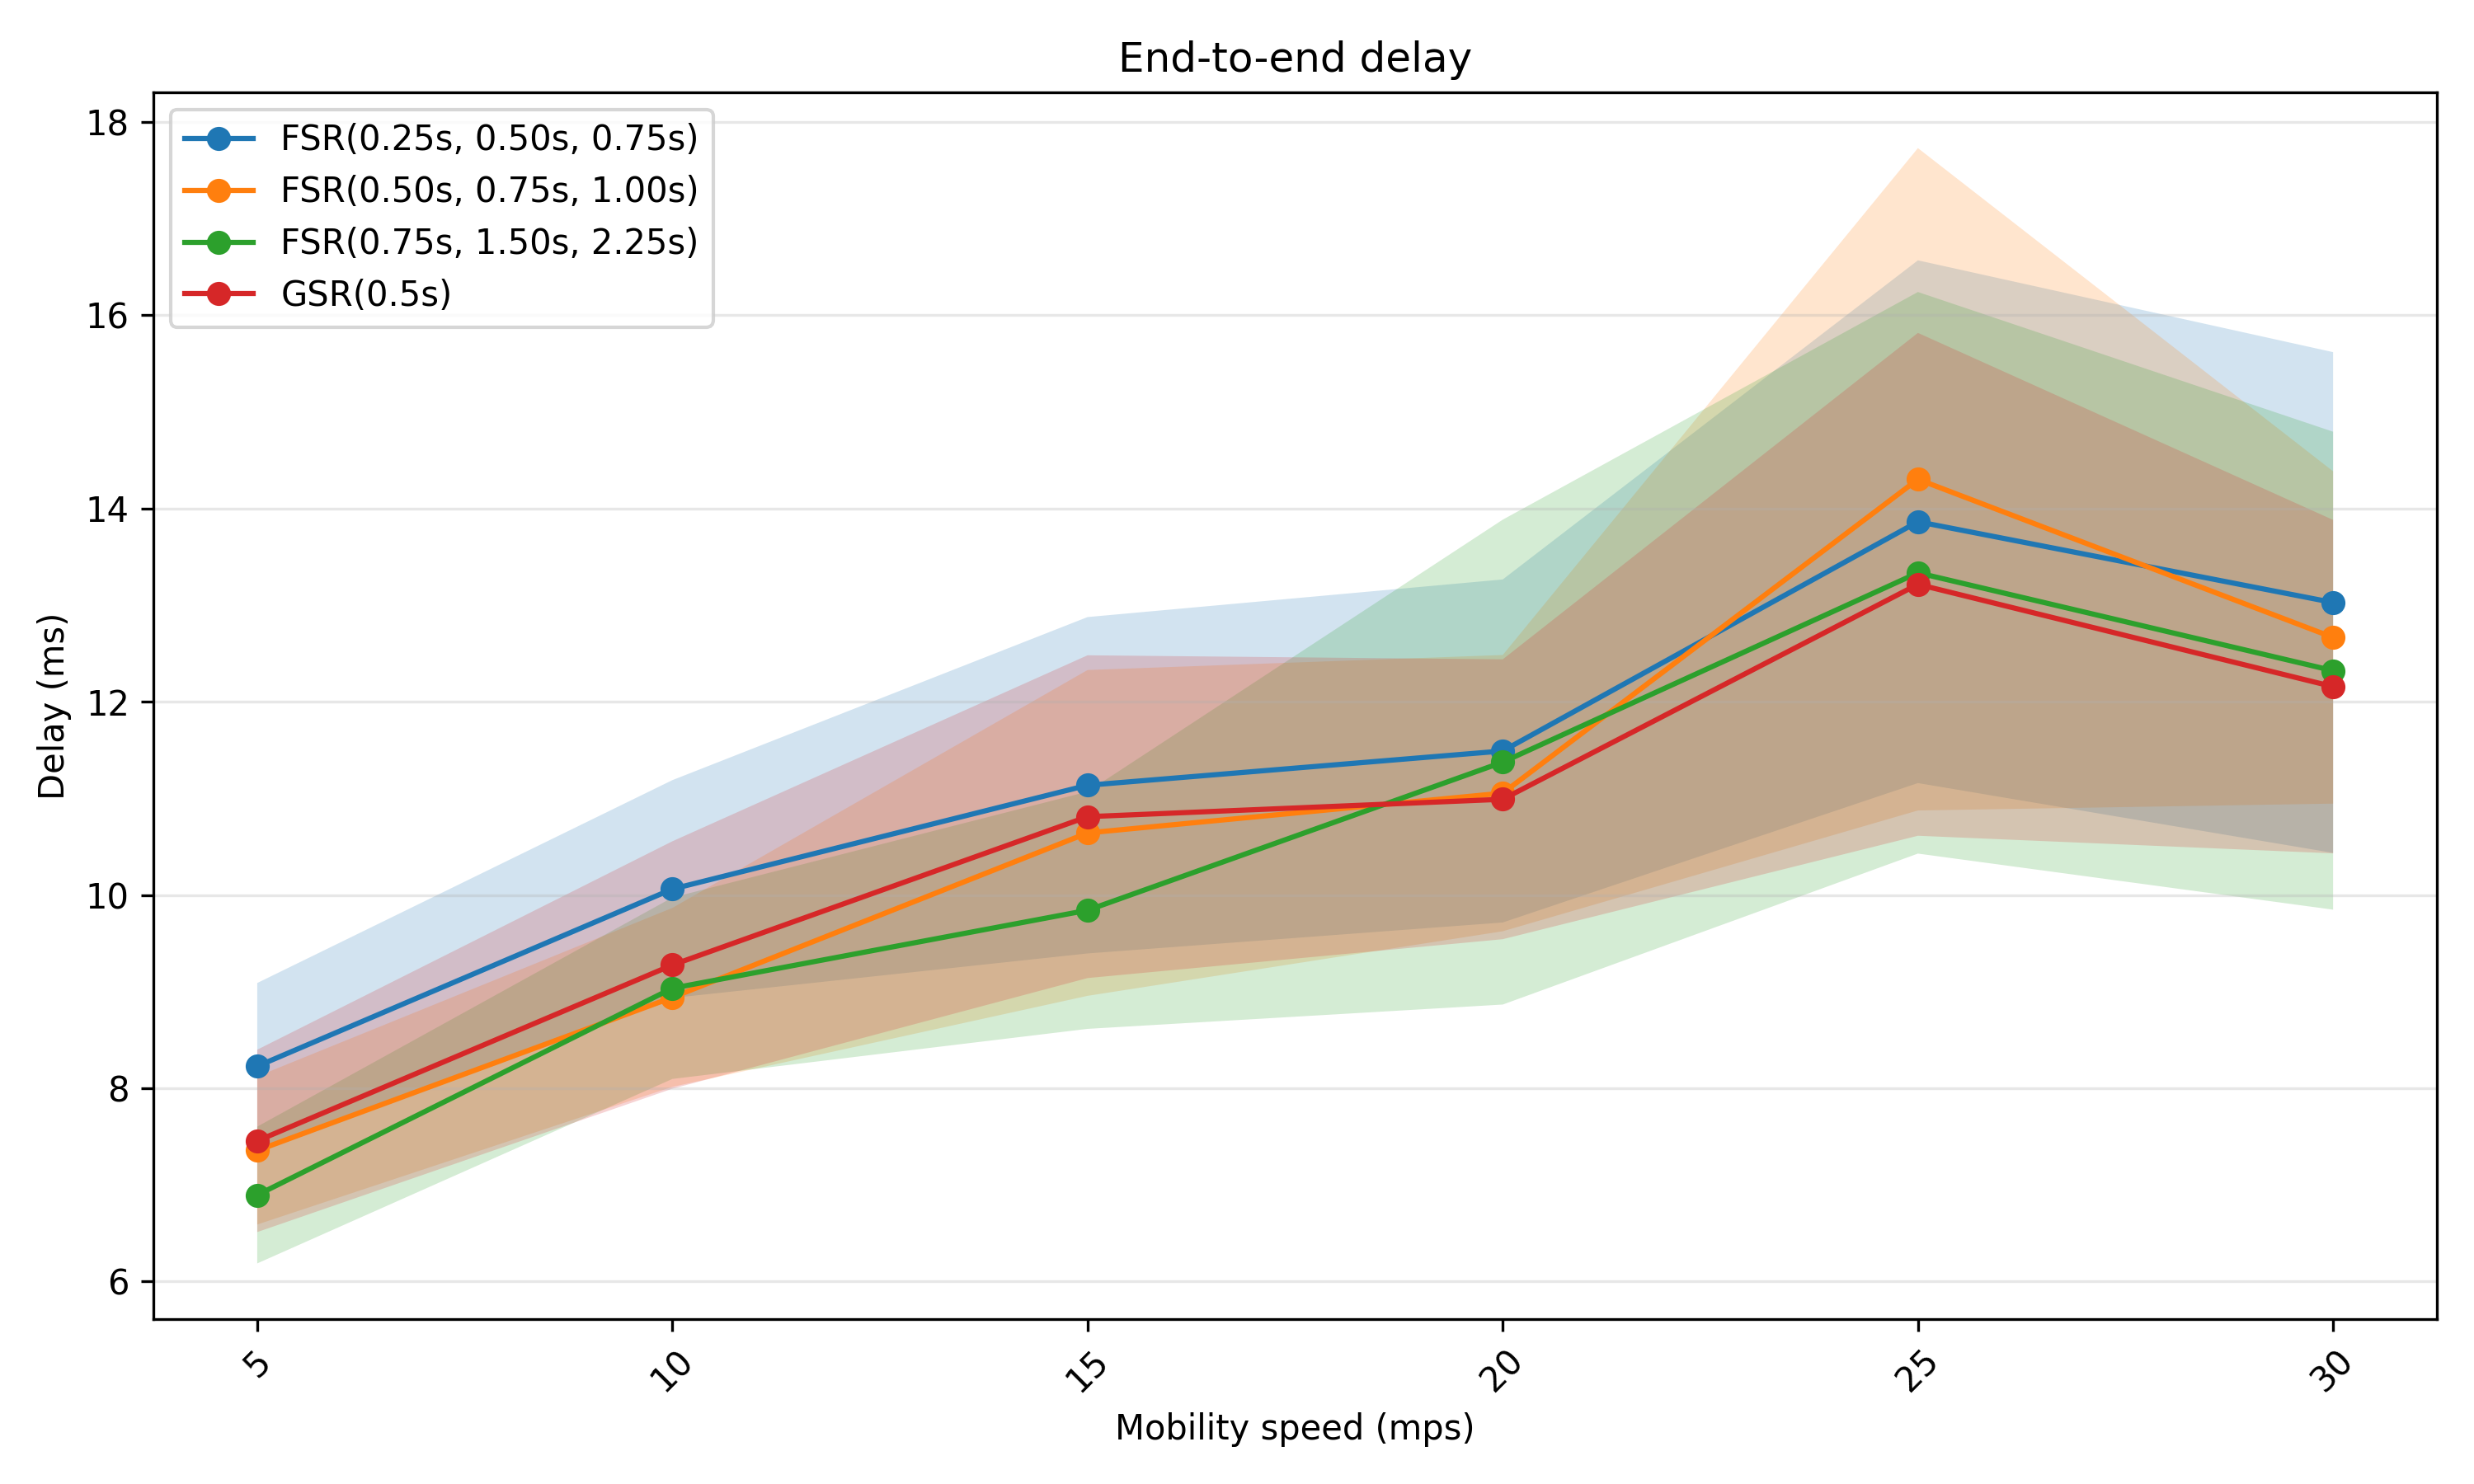
\includegraphics[width=\textwidth]{../figures/speed/end-to-end_delay.png}
        \caption{End-to-end delay}
        \label{fig:delay_speed}
    \end{subfigure}
    \hfill
    \begin{subfigure}[b]{0.45\textwidth}
        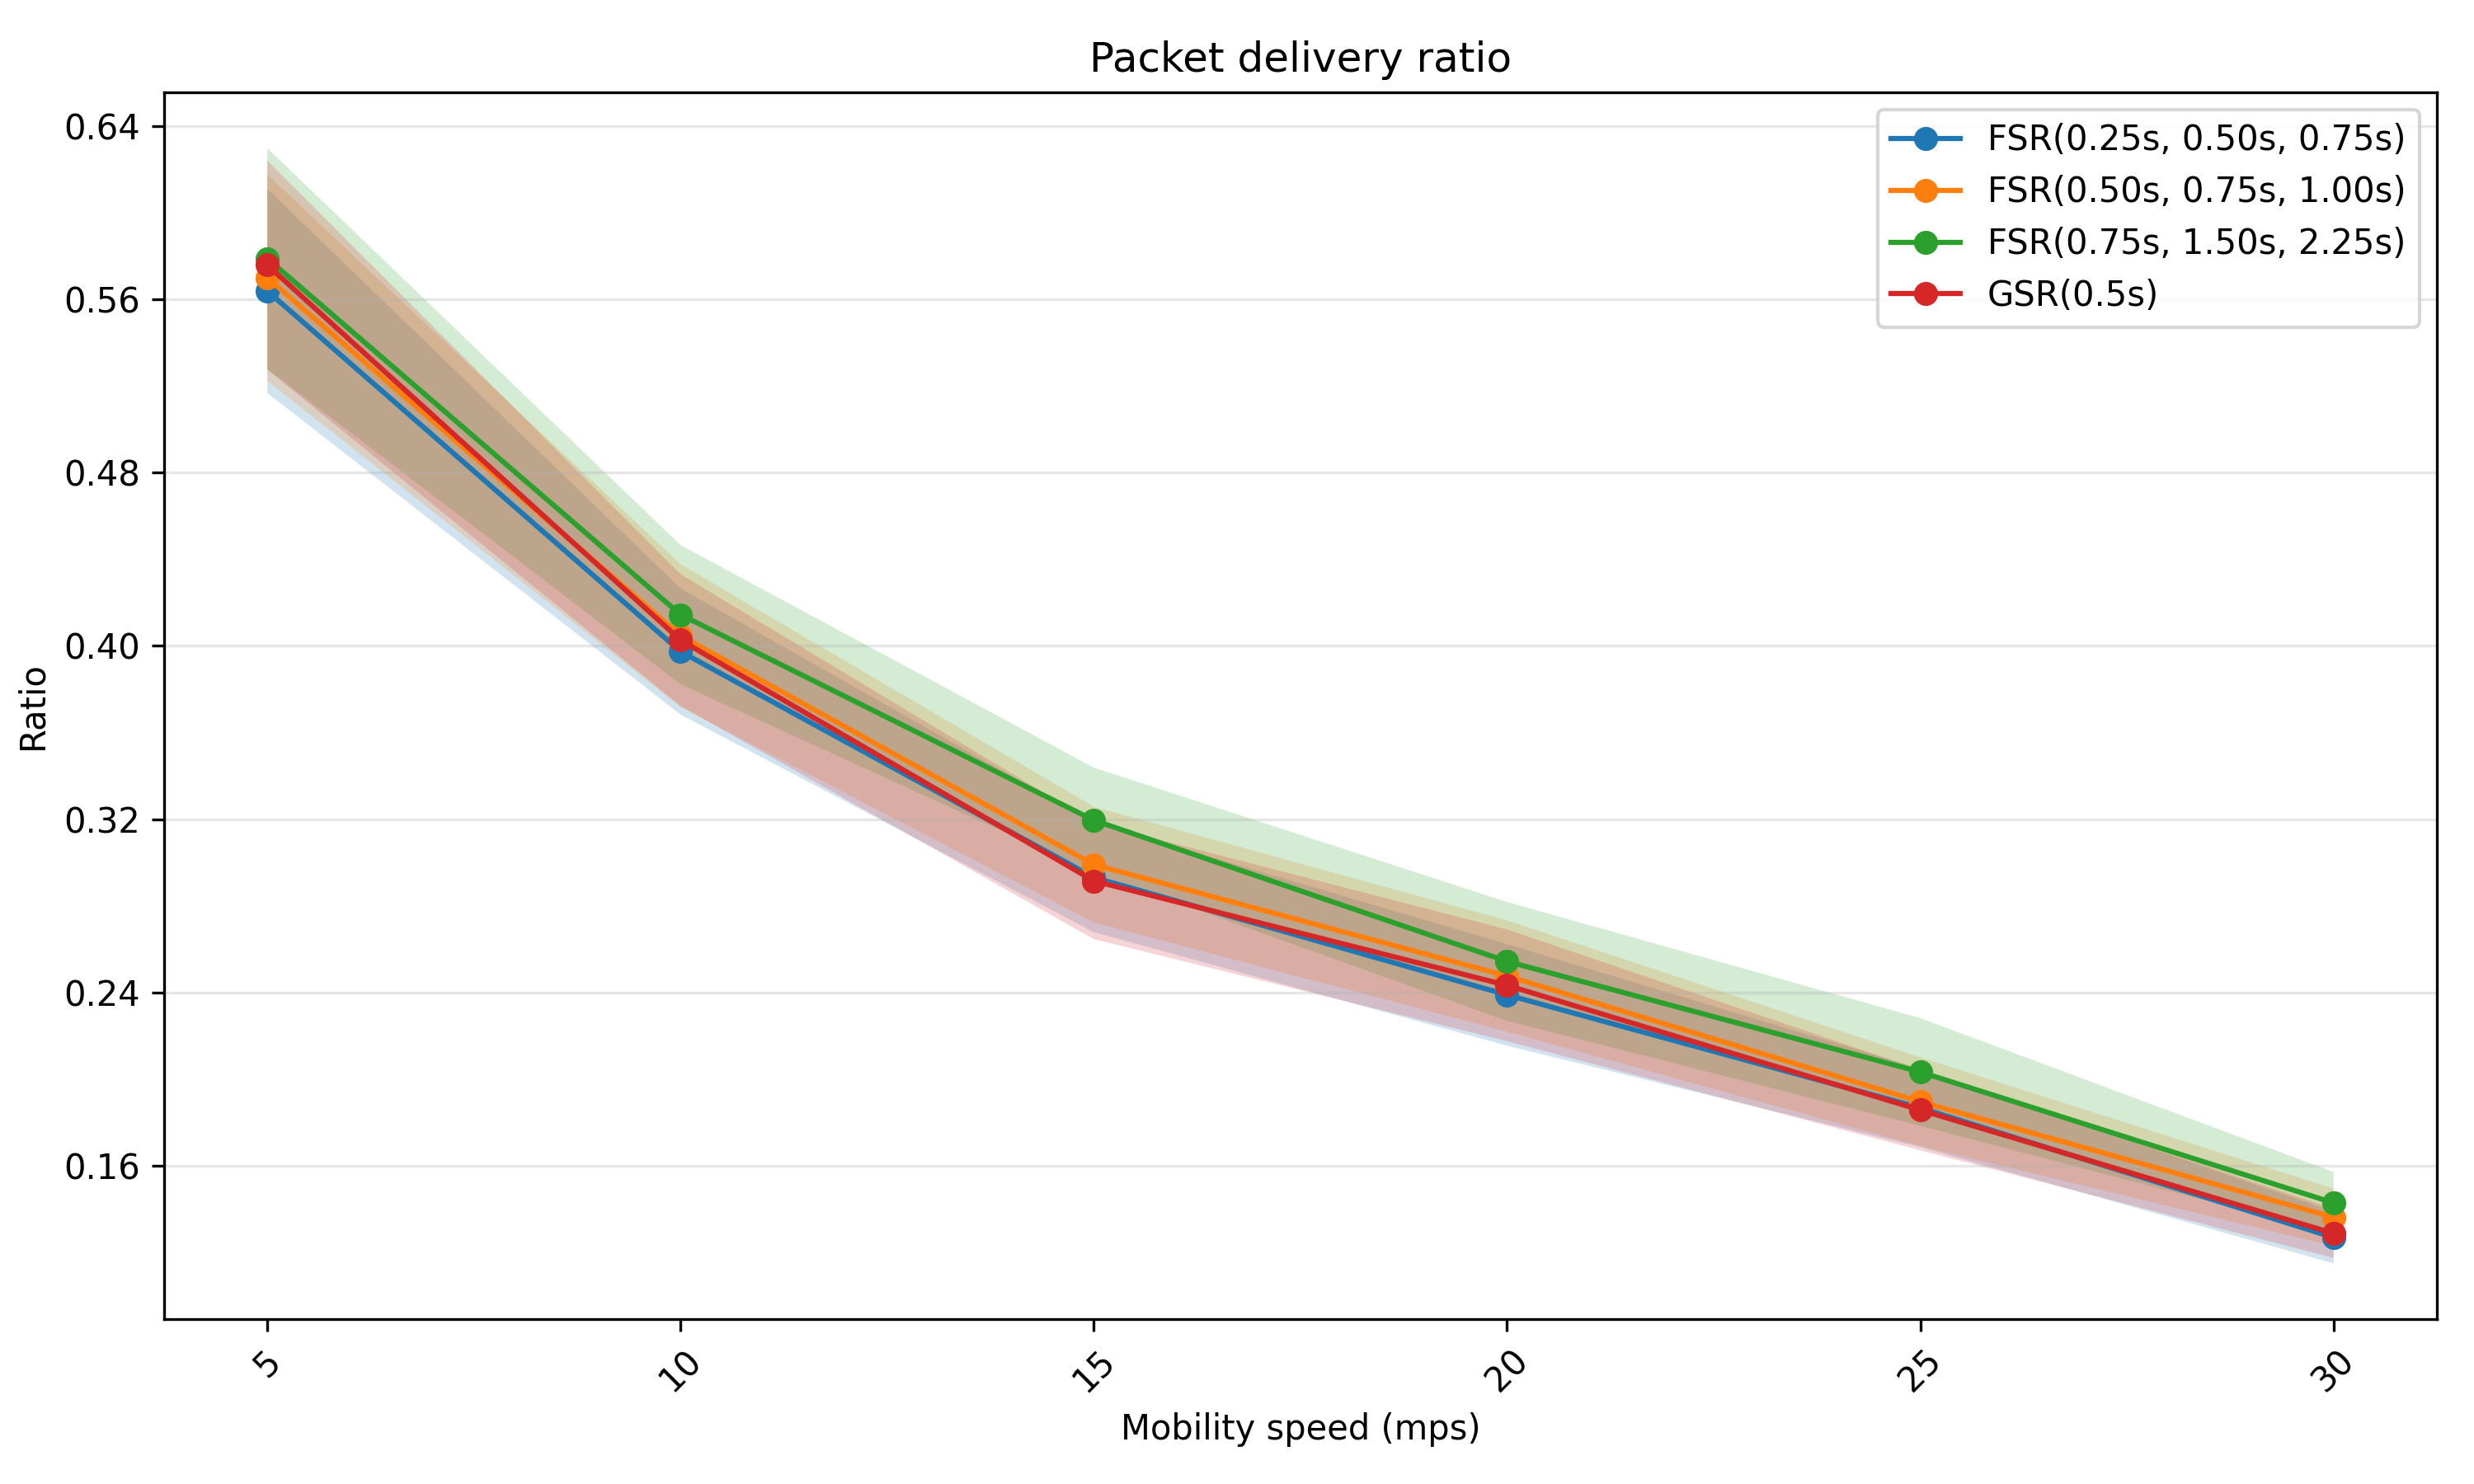
\includegraphics[width=\textwidth]{../figures/speed/packet_delivery_ratio.png}
        \caption{Packet delivery ratio}
        \label{fig:delivery_speed}
    \end{subfigure}
    \begin{subfigure}[b]{0.45\textwidth}
        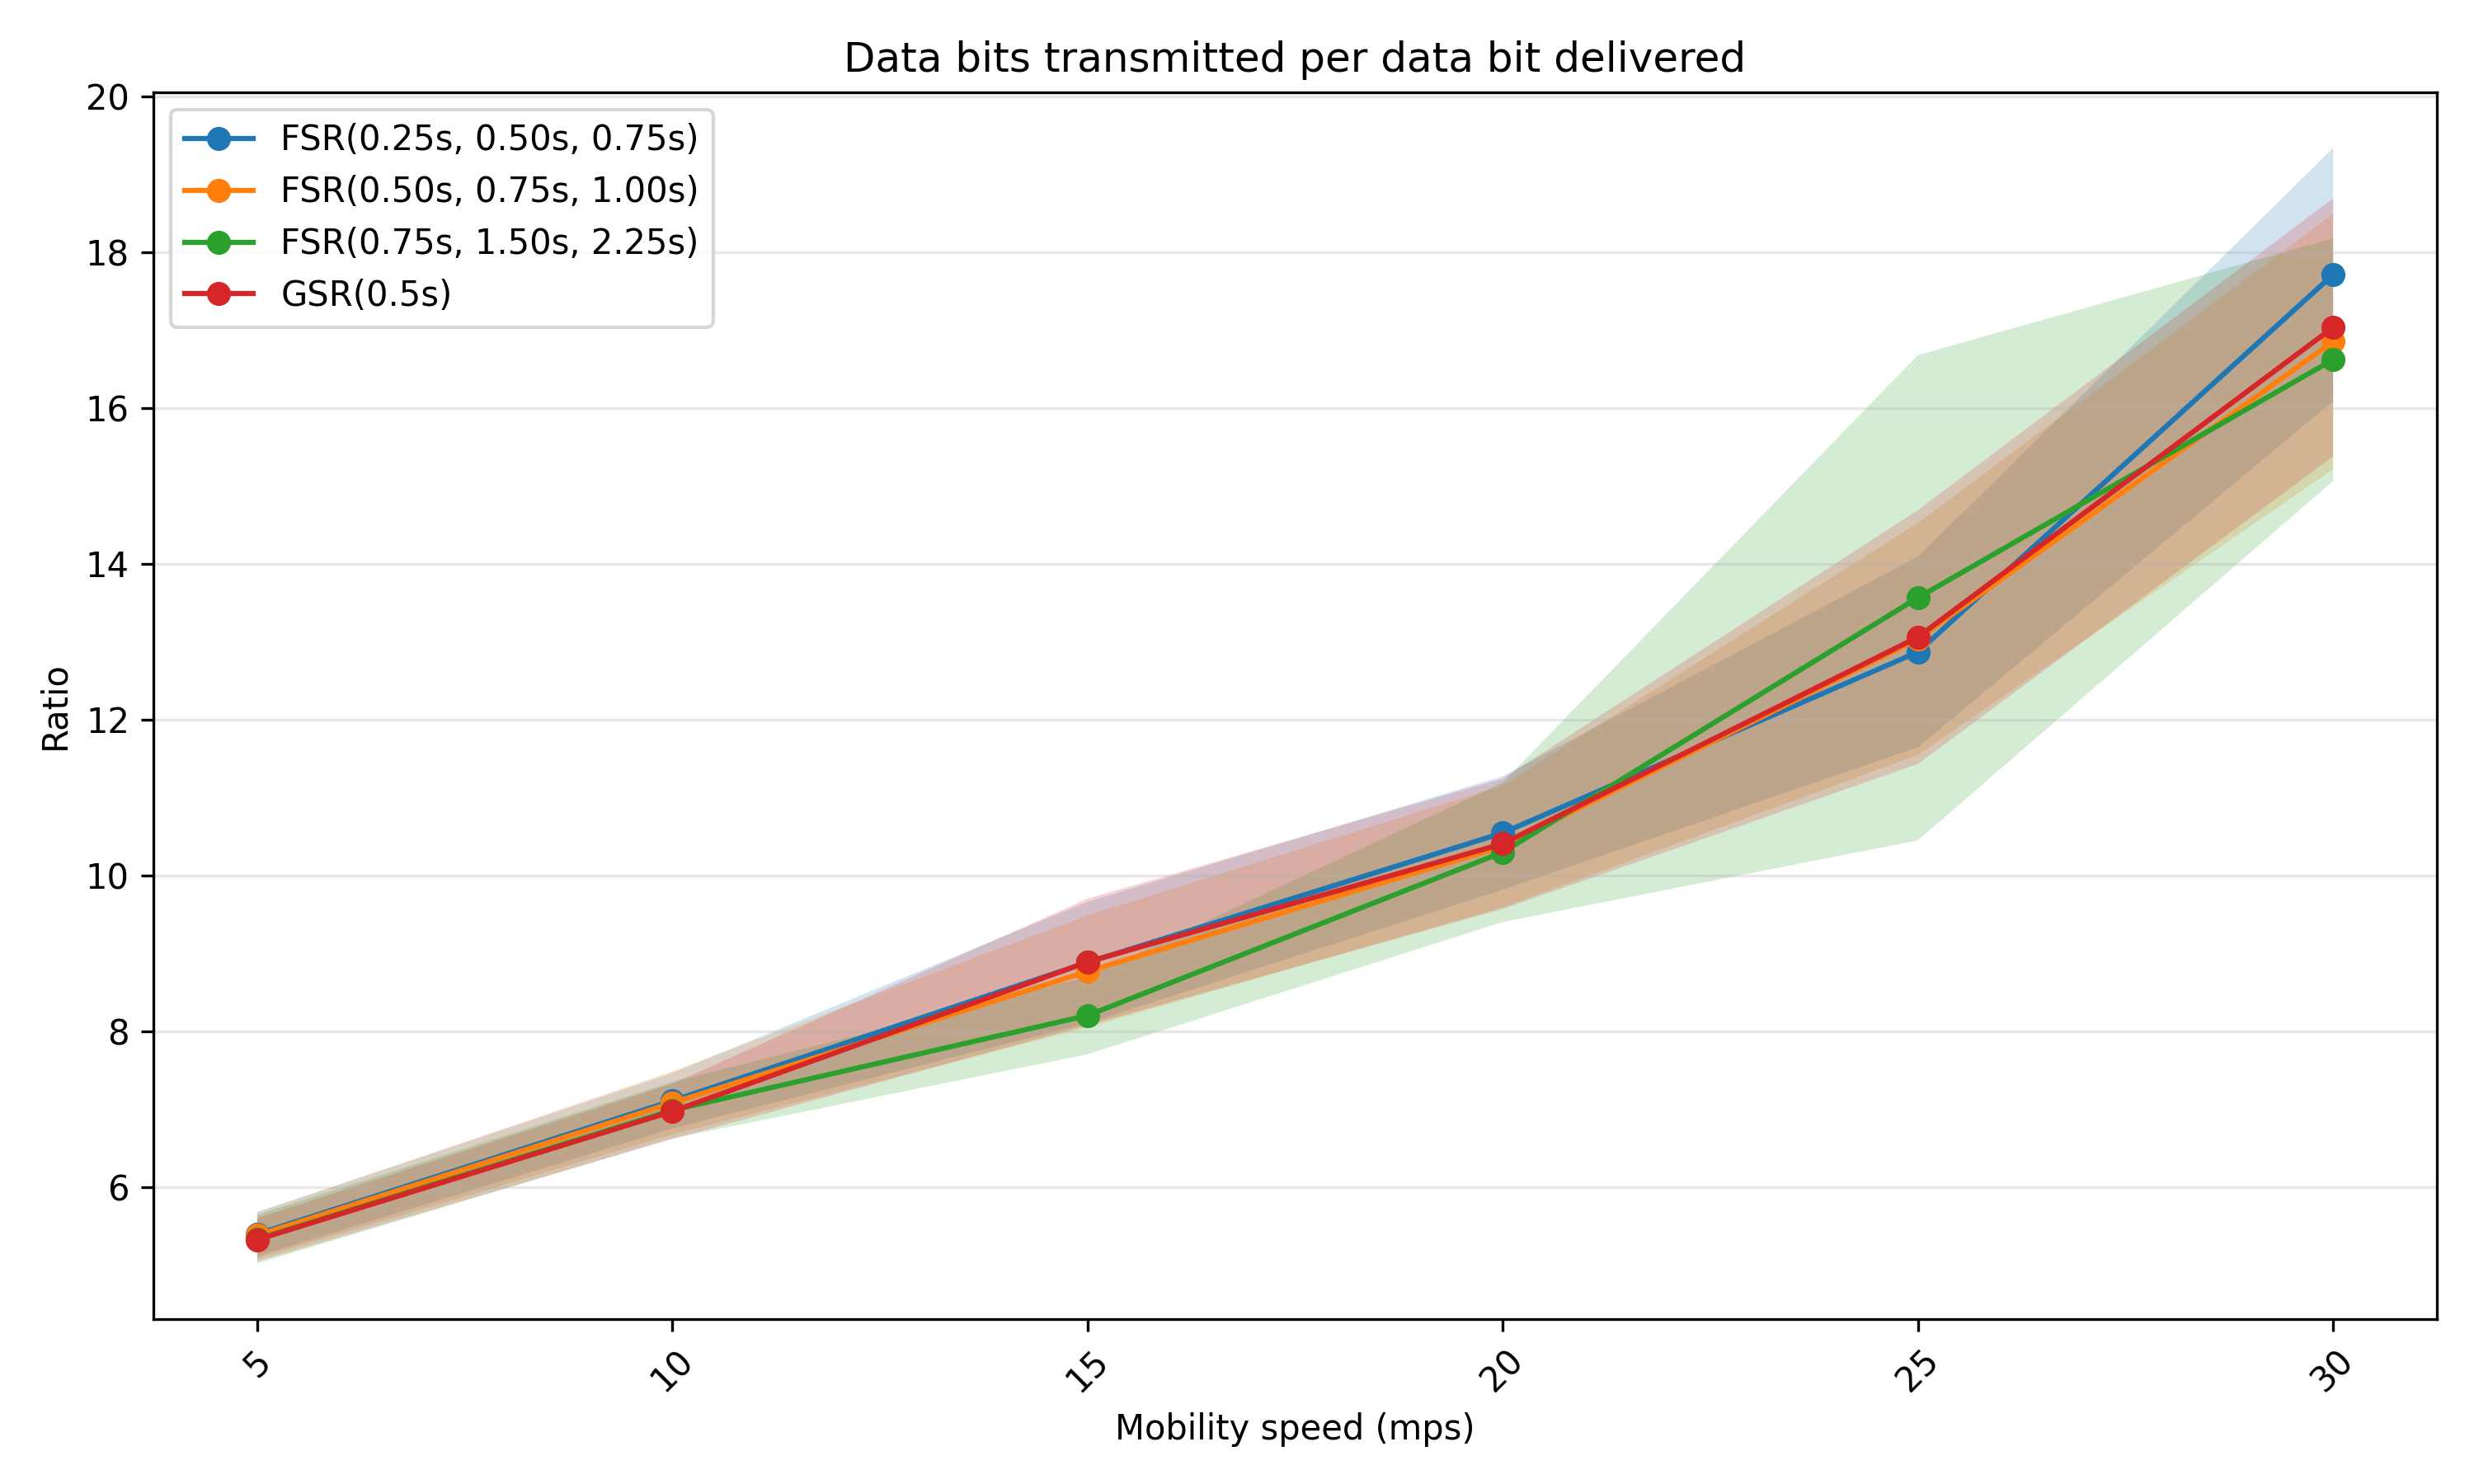
\includegraphics[width=\textwidth]{../figures/speed/data_bits_transmitted_per_data_bit_delivered.png}
        \caption{Data bits transmitted per data bit delivered}
        \label{fig:data_bits_speed}
    \end{subfigure}
    \begin{subfigure}[b]{0.45\textwidth}
        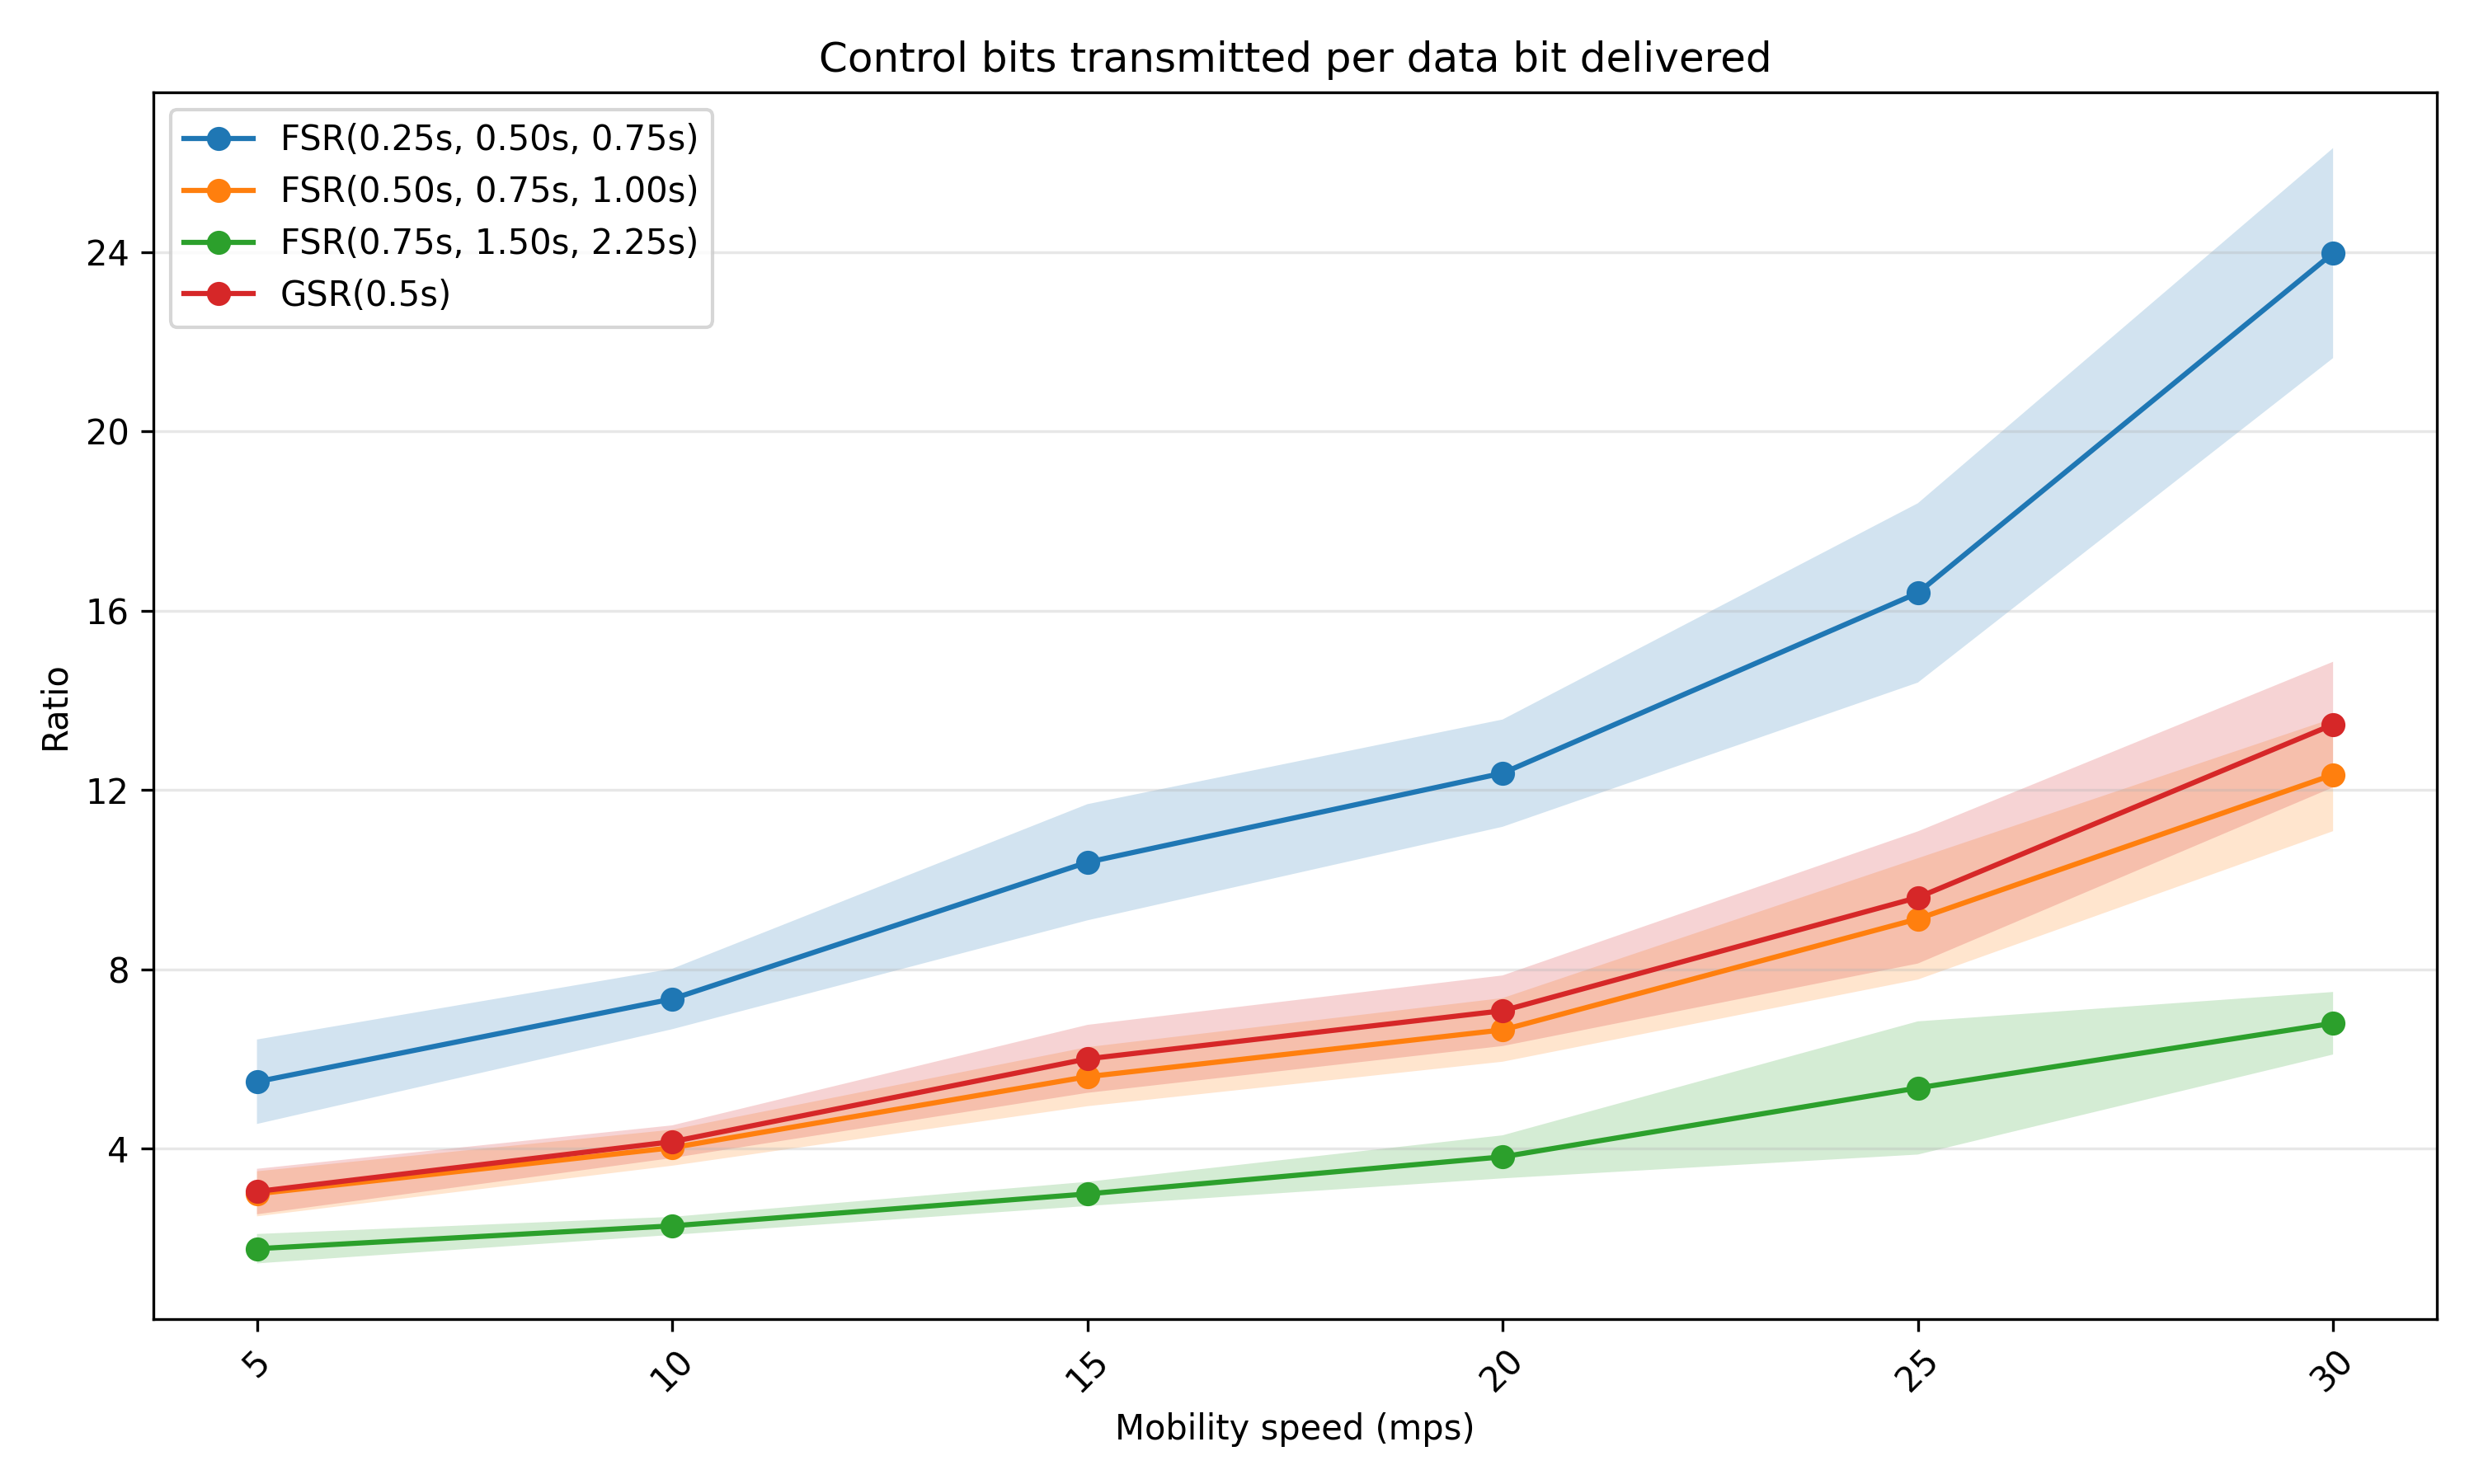
\includegraphics[width=\textwidth]{../figures/speed/control_bits_transmitted_per_data_bit_delivered.png}
        \caption{Control bits transmitted per data bit delivered}
        \label{fig:control_bits_speed}
    \end{subfigure}
    \caption{Minimum speed of mobility}
    \label{fig:speed}
\end{figure}

\section{Conclusion}
From the various parameters studied, we can conclude that the effectiveness of FSR is highly dependent on the network conditions and the configuration of the protocol itself. Lower scope refresh rates lead to better performance in most cases, as they reduce the overhead of control packets and allow for more stable routes. The network size and topological rate of change also play a significant role in the performance of FSR, with larger networks and higher mobility speeds leading to more challenges in maintaining stable routes. Furthermore, the comparison between FSR and GSR shows that the fisheye approach did not yield significant performance improvements, which implies that the expected lower control overhead does not necessarily translate to better performance in all scenarios.

\printbibliography[title={References}]

% appendices use section and subsection numbering
\appendix

\end{document}
